%!TeX root = 2-thermo.tex
\documentclass[main.tex]{subfiles}

\begin{document}

\chapter{Thermodynamic exploration of xenon/krypton separation}
\vspace*{-1\baselineskip}

\section{Simulation of adsorption properties}

\subsection{Geometrical descriptors}

Before going into the details of the adsorption properties themselves, we will first introduce the different simulation techniques used to characterize the internal pore structure of a material key in interpreting the adsorption properties obtained using more complex molecular simulations. All the geometrical descriptors used in this thesis have been calculated using the Zeo++ software;\cite{Zeo++} other tools exist,\ref{First_2013,PoreBlazer} but the use of Voronoi decomposition of the volume speeds up the calculation making it the preferred tool for this task (efficiency gain mainly on volume calculation).~\cite{Rycroft_2009} 

\subsubsection{Pore size}

There are a multitude of pore sizes depending on the point where we measure it, all these pore sizes  compose what we call a pore size distribution. Some specific values are, however, uniquely defined and used to put a single value to characterize pore sized. The pore limiting diameter (PLD) is the diameter of the largest sphere that can diffuse freely in the structure, it is also noted $D_f$. The largest cavity diameter (LCD) corresponds to the diameter of the largest included sphere along a free diffusion path also denoted $D_if$; the global cavity diameter is the diameter of the largest included sphere (not necessarily in a free diffusion path) also denoted $D_i$. The Figure~\ref{fgr:pore_size} illustrates the difference between these pore sizes. 

\begin{figure}[ht]
  \centering
  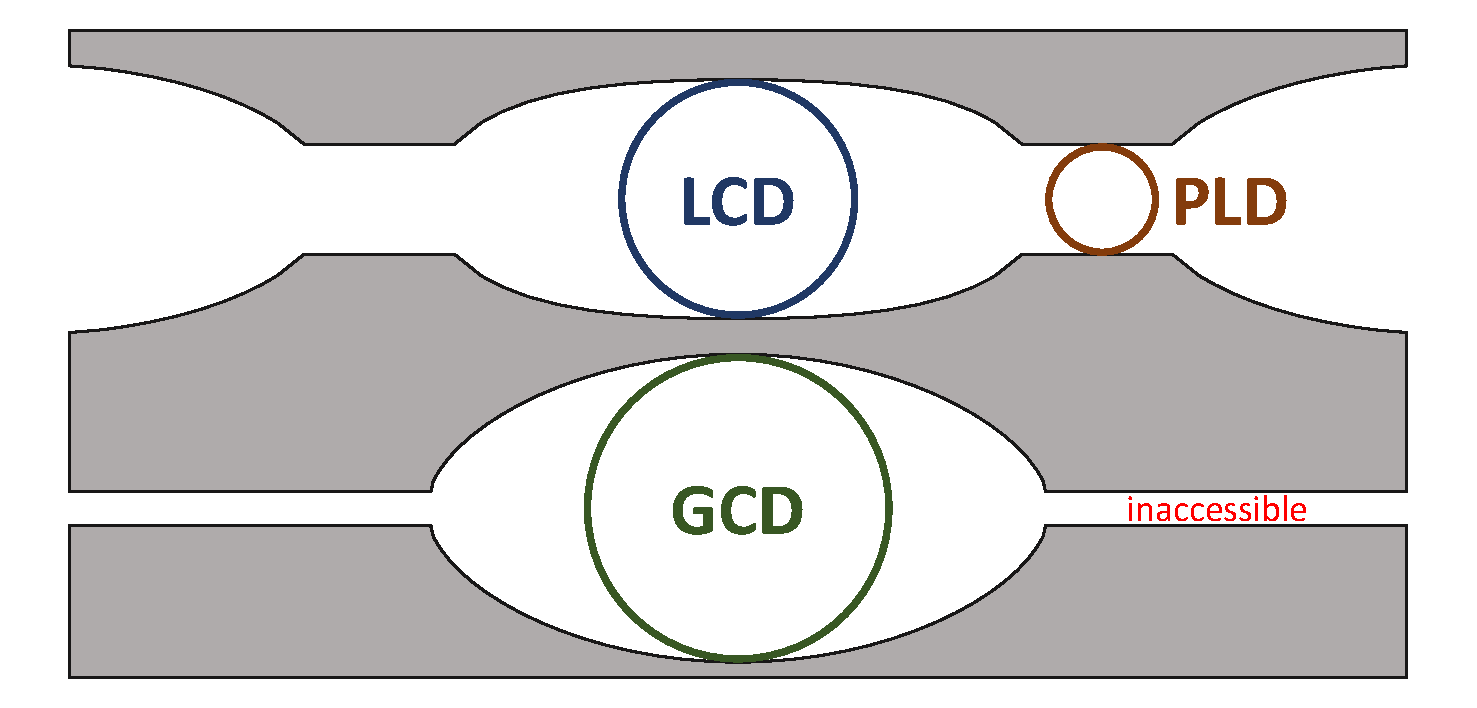
\includegraphics[width=0.7\textwidth]{figures/2-thermo/pores.pdf}
  \caption{Illustration of the different pore sizes PLD, LCD and GLD. \todo{}}\label{fgr:pore_size}
\end{figure}

To define theses pore sizes, we need to first set the radii of the framework atoms that will shape the surrounding pores. These radii can be defined using different methods, the default mode uses the Cambridge database radii. We used a similar approach than the one developed by Hung et al. instead of the default definition.\cite{Hung_2021} All Zeo++ calculations use an atomic radius that corresponds to the distance where the LJ potential reaches $3 k_\text{B} T/2$, for $T = \SI{298}{\kelvin}$. This type of definition can be more easily compared to the molecular simulations.

\subsubsection{Surface Area}

The surface areas are calculated using a random sampling over the surface of the different atom surfaces. The algorithm counts only the points that do not overlap with another atom. For each atom we can therefore calculate an adsorbable surface. By summing up all the surfaces, we finally have the surface area. This Shrake-Rupley algorithm has been developed since 1973.\cite{Shrake1973} the By defining a probe, the Voronoi tessellation defines the accessible and the non-accessible areas of the structure. Depending on where the surfaces are, they are either counted in the accessible or the non-accessible surface areas. In this chapter, we will use the accessible surface area defined by a probe of $1.2$~\si{\angstrom}; this is a computational equivalent of the experimental \ce{N2} BET surface area.

\begin{figure}[h!]
  \centering
  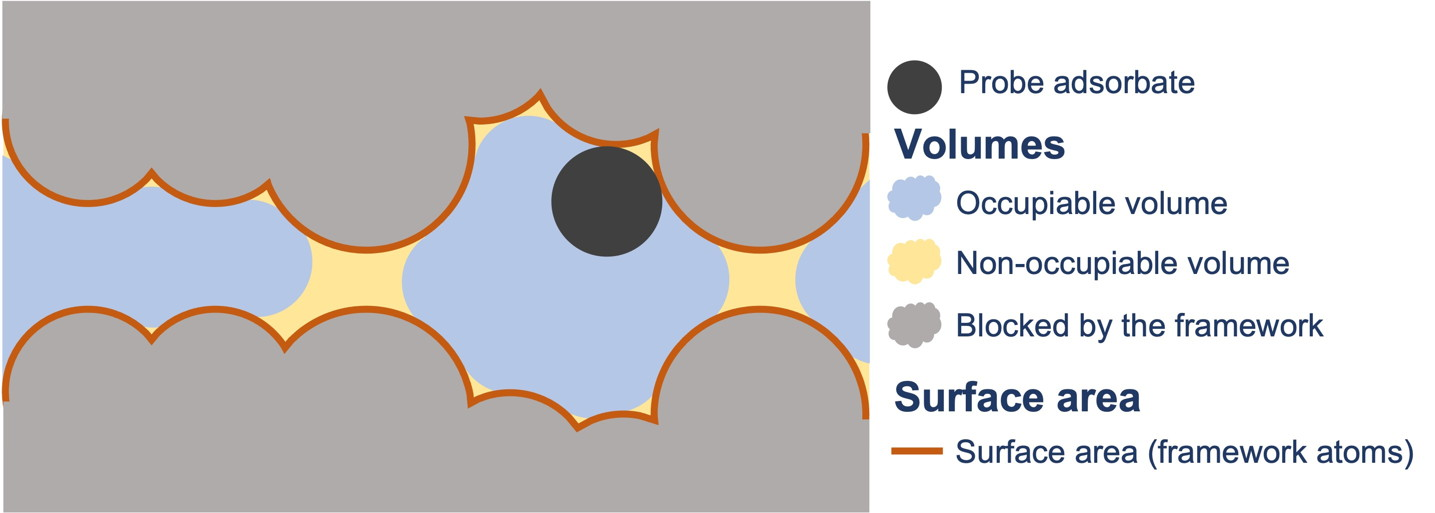
\includegraphics[width=0.7\textwidth]{figures/1-screening/Pore_descriptors.jpg}
  \caption{Illustration of the pore surface area and volume in a nanoporous material. As illustrated, there are different definitions of the pore volume: we can either consider the whole volume of the pores or the volume occupiable by a given probe. The surface area also changes depending on the definition. Studies have shown that occupiable volume has a better accordance with experimental data.\cite{vol_Ongari2017}}\label{fgr:pores}
\end{figure}

\subsubsection{Pore volume and porosity}

The pore volume is calculated by random sampling of the accessible and inaccessible Voronoi cells. Similar algorithm, random sampling over a regular mesh. If the probe does not overlap with a framework atom, then it is counted in $N$. The ratio of this final $N$ and the total number of points sampled gives the fraction of the pore volume. This ratio is called the void fraction or the porosity. Using the Voronoi decomposition, we can also define the accessible and non-accessible void fractions.\todo{}

\subsection{Mixture adsorption simulations: Grand Canonical Monte Carlo}

%intro 
As explained before, we can think of adsorption as a gas--solid or liquid--solid interfacial phenomenon, the adsorbate phase fills the accessible pore volumes depending on the physical conditions the material is put under. No simple model can predict how the adsorbates would interact with the pore surface, how many of them can fit in, what configuration is the most stable, etc. To answer these questions, we can evaluate all possible adsorption configurations that would undeniably have different numbers of adsorbate, and only keep the most thermodynamically plausible ones. To do so, these configurations will have to follow a given probability distribution, the grand canonical ensemble probability for instance, because it allows the variation of the number of molecules (adsorbate molecules) and the total energy. With the help of a Monte Carlo simulation, we can vary the energy and the loading inside the pores so that the distribution of configurations $c$ follows this probability law: 
\begin{equation}
  P_c = \dfrac{1}{\Xi}e^{-\beta\left(E_c-\mu N_c\right)} 
  \label{eqn:gc}
\end{equation}
where $E_c$ and $N_c$ are respectively the energy and the number of adsorbate particles in the configuration $c$. Normally the energy and the number of molecules of all particles should be considered, but for now, since the whole system is considered rigid we will only focus on the adsorbate molecules. The chemical potential $\mu$ and the temperature $T$ inside $\beta$ correspond to the ones of the gas phase in equilibrium with the adsorbent material. And the pressure and volume $V$ are considered fixed under the rigidity assumption. The grand canonical partition function $\Xi(\mu,V,T)$ will then be the following sum over all possible configurations: 
\begin{equation}
  \Xi(\mu,V,T) = \sum_c e^{-\beta\left(E_c-\mu N_c\right)} 
\end{equation}
This multiplicative constant does not need to be known in the Monte Carlo simulation we will describe now. 

Beyond these theoretical considerations, the grand canonical Monte Carlo simulation, referring to a Metroplis-Hastings Monte Carlo algorithm in the context of the grand canonical thermodynamic ensemble, will need several key characteristics in order to fulfill the previous claims on the probability distribution of the configurations. Monte Carlo (MC) refers to the randomness inherent to the gambling games of the eponymous casino on the azure coast of Monaco. The MC simulations are therefore relying on randomly generating atomic configurations; however in order to do it efficiently, we need to stay as much as possible in the physically possible atomic space, while exhaustively exploring all the chemical configurations. 
In molecular simulations, to do so, only the initial configuration $c_0$ is really randomly generated, but then the algorithm has different rational moves to change the configuration with a controlled amount of randomness. The second key feature (acceptance or rejection condition) was introduced by Metropolis and co-workers that allows to reproduce any distribution with an unknown multiplicative prefactor.\cite{Metropolis1949} The configuration $c_1$ resulting of the random move is evaluated by calculating the transition probability (like in a Markov chain) or acceptance rate $acc(c_0 \rightarrow c_1)$: 
\begin{equation}
  acc(c_0 \rightarrow c_1) = \min\left(1, e^{-\beta\left(E_{c_1}-E_{c_0}-\mu \left(N_{c_1}-N_{c_0}\right)\right) }\right)
\end{equation}
Any move that has a greater probability of occurring is always accepted, if the probability is lower than the acceptance rate depends on the probability ratio.
The multiplicative prefactor has no influence on the algorithm, we do not need to know the chemical space to explore beforehand, which is a valuable simplification. This sequence of a Markov-type chain can then be used to approximate the probability distribution of the grand canonical ensemble we seek to describe in the equation~\ref{eqn:gc}.


\begin{figure}[ht]
  \centering
  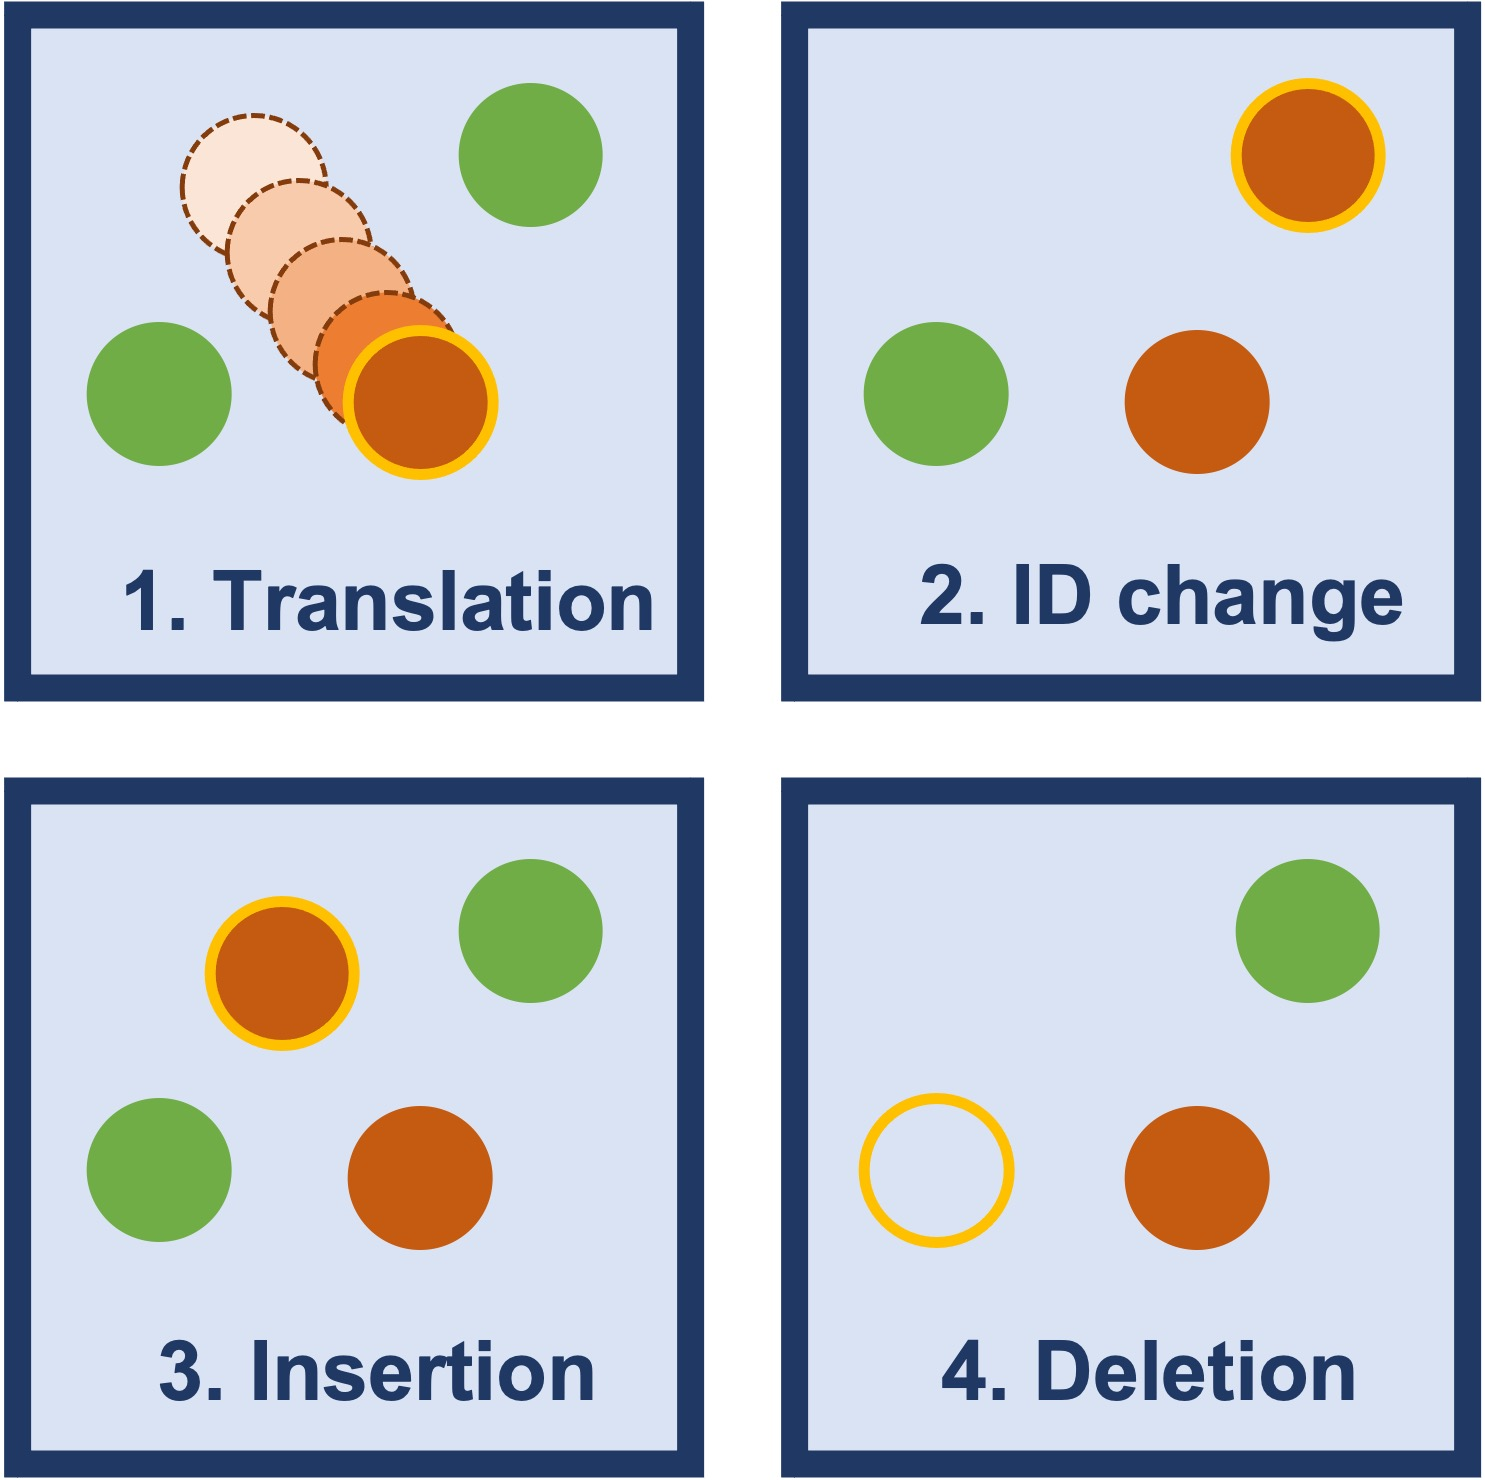
\includegraphics[width=0.99\textwidth]{figures/2-thermo/MC_moves.jpg}
  \caption{MC moves for monoatomic atoms with multiple components}\label{fgr:mc}
\end{figure}

To complete the description of the grand canonical Monte Carlo (GCMC) simulation we are interested in, let us now consider the different MC moves used to generate a configuration from another. Depending on the parameterization, these moves have different probabilities of occurring. For monoatomic atoms only four moves are relevant (see Figure~\ref{fgr:mc}): (1) the translation of a randomly chosen molecule with a displacement randomly chosen within a given radius, (2) the change of identity of a randomly chosen molecule into another, (3) the insertion of an adsorbate molecule and (4) the deletion of an adsorbate molecule. We deliberately omitted the rotations of the adsorbate because of the spherical symmetry of noble gases and the change of volume since the flexibility of the material framework is neglected. 

By using a GCMC algorithm, we can now generate a set of configurations according to their probability of occurrence. Because the probability law is directly taken from equation~\ref{eqn:gc}, the series of configurations describe the thermodynamic equilibrium state of a nanoporous material in contact with a reservoir of a xenon-krypton mixture at a given composition, pressure and temperature. Different thermodynamic quantities can be derived from ensemble averaging: the averaging loading or uptake at a given pressure (several pressures give the isotherm) and the isosteric heat of adsorption of each adsorbate (Xe and Kr). The ratio of the uptakes $q$ informs on the selectivity $s$ of the thermodynamic separation process: 
\begin{equation}\label{eq:selec}
  \boxed{
  s = \dfrac{q\ex{Xe}}{q\ex{Kr}}\times\dfrac{y\ex{Kr}}{y\ex{Xe}}
  }
\end{equation}
where $y\ex{Xe}$ and $y\ex{Kr}$ designate respectively the mole fractions of Xe and Kr in the gas phase reservoir.

To characterize a separation process, we theoretically only need to perform a GCMC calculation at every pressure conditions that we are interested in. However, this type of simulation requires a lot of time to converge since we need to test out a lot of insertion/deletion moves to accurately estimate the number of adsorbed molecules and the composition of the mixture. Hence, faster methods (machine learning) are developed to estimate the selectivity at any pressure conditions.\cite{Simon_2015,Kang_2023} If we are interested in the infinite dilution case, faster methods are already available, we are now going to introduce the Widom insertion that can estimate the adsorption performances at infinite dilution by estimating the Henry adsorption constant.


\subsection{Infinite dilution adsorption: Widom insertion}

In 1963, the professor B. Widom introduced a simple method of calculation of thermodynamic properties in a material or fluid mixture.\cite{Widom1963} Generally, this method allows accessing to the difference of internal energy before and after the insertion of a Widom test particle while fixing all other particles, therefore comparing the N-particle and (N+1)-particle states. This difference of energy $\Delta \Phi$ can then be used to deduce the excess free energy associated to it $\Delta F\e{exc} = -k\e{B} T \ln\left(\langle \exp(- \beta\Delta \Phi) \rangle\right)$, which corresponds to the excess chemical potential induced by the addition of a particle. In the domain of fluid phase equilibrium, Widom insertion is the most straightforward method to calculate a chemical potential value; however it has drawbacks in liquid-like phases because the insertable space is very narrow, and no relaxation is implemented to account for the reorganization of the surrounding particles.\cite{Nezbeda_1991} In our case, we will be only interested in the insertion from 0 to 1 particle, where no problems of overlapping between adsorbate particles can happen. Widom insertion is in our case only a random insertion of an adsorbate into an empty nanoporous framework. By randomly sampling the void space, we obtain a distribution of interaction energies $\mathcal{E}\e{int}$, the average of the Boltzmann weights associated is directly proportional to the adsorption free energy $\Delta G\e{ads}$ and the Henry adsorption constant $K\e{H}$. By taking the Boltzmann average of the interaction energies, we can also compute the adsorption enthalpy $\Delta H\e{ads}$. All these quantities stay only valid at infinite dilution, for higher quantities of adsorbates the previously described GCMC technique should be used.  

In the infinite dilution case, this test particle insertion technique is similar to a random sampling of the adsorbable space inside a material. If the sampling is thorough enough, we can derive the following definitions of $\Delta G\e{ads}$ (equation~{eqn:gibbs}), $K\e{H}$ (equation~{eqn:henry}) and $\Delta H\e{ads}$ based on a complete sampling of the interaction energies $\mathcal{E}\e{int}$. 

The adsorption Gibbs free energy $\Delta G\e{ads}$ is equal to the excess free energy previously calculated in a Widom insertion since the structure is rigid and $PV$ does not fluctuate ($G = F + PV$). 

\begin{equation}\label{eq:ads_gibbs}
  \boxed{
  \Delta G\e{ads} = -RT \ln\left(\langle \exp(-\mathcal{E}\e{int}/RT) \rangle\right)
  }
\end{equation}

To derive the Henry constant $K\e{H}$, we need to consider an ideal gas. The number of adsorbed molecules $n\e{ads}$ can be expressed using the bulk density of the gas $\rho\e{ads,bulk}$ and the volume of the pores $V\e{pore}$:

\begin{equation}\label{eqn:1}
    n\e{ads} = \rho\e{ads,bulk} \times V\e{pore}  
\end{equation}

The pore volume can be seen as the continuous sum of each voxel times the Boltzmann probability of presence, which is represented by the following integral of the Boltzmann factors. This integral can then be changed to the average of the Boltzmann factors:

\begin{equation}\label{eqn:vpore}
    V\e{pore} = \int_V \exp\left(- \mathcal{E}\e{int}(\textbf{r})/RT\right) d\textbf{r} = V \langle \exp\left(-\mathcal{E}\e{int}/RT\right) \rangle
\end{equation}

Let us apply the equation~\ref{eqn:vpore} and the perfect gas equation of state $P = \rho\e{ads,bulk}RT$ on the bulk gas in equilibrium, we can change the equation~\ref{eqn:1} to:

\begin{equation}
    \dfrac{n\e{ads}}{V} = \dfrac{P}{RT} \langle \exp\left(-\mathcal{E}\e{int}/RT\right) \rangle
\end{equation}

If we now consider the gravimetric loading $L\e{ads}$ (in~\si{\milli\mole\per\gram}), we need to divide the equation by mass density of the framework $\rho_f$:

\begin{equation}
  L\e{ads} = \dfrac{n\e{ads}}{V\rho_f} = \dfrac{\langle \exp\left(-\mathcal{E}\e{int}/RT\right) \rangle}{\rho_fRT} P
\end{equation}

Since the Henry's law is described by $L\e{ads}=K\e{H} \times P$, we have the final relation between the Henry adsorption constant and interaction energy distribution.

\begin{equation}\label{eqn:henry}
    \boxed{
    K\e{H} = \dfrac{\langle \exp\left(-\mathcal{E}\e{int}/RT\right) \rangle}{\rho_fRT} = \dfrac{1}{\rho_fRT} \exp\left(-\dfrac{\Delta G\e{ads}}{RT}\right)
    }
\end{equation}

Note that the $\rho_f$ factor comes from the use of a gravimetric loading expressed in~\si{\milli\mole\per\gram} and is not always present in the different derivations of the literature.\cite{PoreBlazer} The $RT$ factor comes from the perfect gas assumption we made, which is a good approximation in the noble gas case. 

Finally, if we consider an adsorption equilibrium (e.g., $\text{Xe}\e{(g)} \rightleftharpoons \text{Xe}\e{(ads)}$), we can define an equilibrium constant $K\e{ads} = x\e{ads}/y\e{gas}$ where $x\e{ads}$ is the mole fraction in the adsorbed phase and $y\e{gas}$ the mole fraction in the gas phase for a given compound (e.g., Xe). For a pure gas ($y\e{gas}=1$) at infinite dilution, we can apply the Henry's law to derive the following relation:

\begin{equation}\label{eqn:eq_cst}
  K\e{ads} = \dfrac{n\e{ads}}{n\e{site}y\e{gas}} = \dfrac{K\e{H}P\rho_fV}{n\e{site}} = PV \dfrac{\langle \exp\left(-\mathcal{E}\e{int}/RT\right) \rangle}{n\e{site}RT}
\end{equation}
where $n\e{site}$ is the number of sites considered constant since it is much higher than $n\e{ads}$ at infinite dilution.

Now by applying the Van't Hoff equation to this infinite-dilution adsorption equilibrium constant $K\e{ads}$, we can derive an expression of the adsorption enthalpy at infinite dilution:

\begin{equation}
  \Delta H\e{ads} = -R\dfrac{\dd \ln\left(K\e{ads}(T)\right)}{\dd (1/T)}
\end{equation}

Then by decomposing the logarithm on the fraction of equation~\ref{eqn:eq_cst}, 
\begin{equation}
  \Delta H\e{ads} = -\dfrac{\dd \ln\left(PV/n\e{site}\right)}{\dd (1/T)} - R\dfrac{\dd \ln\left(\langle \exp\left(-\mathcal{E}\e{int}/RT\right) \rangle\right)}{\dd (1/T)} - R\dfrac{\dd \ln\left(1/T\right)}{\dd (1/T)}
\end{equation}

Then, $PV/n\e{site}$ being a constant, we can reduce the expression to two derivatives, the first one being the logarithmic derivative of itself ($1/T$) and the second being the logarithmic derivative of the sum of the exponential terms. 

\begin{equation}
  \Delta H\e{ads} = 0 - R\dfrac{\dd \ln\left(\langle \exp\left(-\mathcal{E}\e{int}/RT\right) \rangle\right)}{\dd (1/T)} - RT
\end{equation}

Knowing that for any function $f$ the logarithmic derivative equals the quotient of its derivative $f'$, $\dfrac{\dd \ln\left(f\right)}{\dd x}=f'/f$, we can calculate the derivative of the average of the Boltzmann factors $\langle \exp\left(-\mathcal{E}\e{int}/RT\right) \rangle$:

\begin{equation}
  \Delta H\e{ads} = -R\dfrac{1}{\frac{1}{N}\sum e^{-\frac{\mathcal{E}\e{int}}{RT}}} \frac{1}{N}\sum \dfrac{\dd \exp\left(-\mathcal{E}\e{int}/RT\right)}{\dd (1/T)} - RT
\end{equation}
where N corresponds to the number of points where the Widom particle has been inserted.
The exponential derivative makes the energy factors come out, and we get the following expression:
\begin{equation}
  \Delta H\e{ads} = -R\dfrac{1}{\sum e^{-\frac{\mathcal{E}\e{int}}{RT}}} \sum - \frac{\mathcal{E}\e{int}}{R} e^{-\frac{\mathcal{E}\e{int}}{RT}} - RT
\end{equation}

With some simplification, we can express the adsorption enthalpy $\Delta H\e{ads}$ as a Boltzmann average of the interaction energies minus a term $RT$ that comes from the ideal gas assumption (perfect gas equation of state).

\begin{equation}\label{eq:ads_enthalpy}
  \boxed{
  \Delta H\e{ads} = \dfrac{\sum \mathcal{E}\e{int}e^{-\frac{\mathcal{E}\e{int}}{RT}}}{\sum e^{-\frac{\mathcal{E}\e{int}}{RT}}} - RT
  }
\end{equation}

% entropy from free energy and enthalpy
From the values of the adsorption free energy and enthalpy, we can now deduce the adsorption entropy $\Delta S\e{ads}$ using the definition of the Gibbs free energy ($G = H-TS$):
\begin{equation}\label{eq:ads_entropy}
  \boxed{
  \Delta S\e{ads} = \dfrac{1}{T} \left(\Delta H\e{ads} - \Delta G\e{ads} \right)
  }
\end{equation}

%selectivity
We already defined the selectivity as the ratio of the proportion of Xe/Kr in the adsorption phase to the proportion in the gas phase in the equation~\ref{eq:selec}. At infinite dilution, we can rewrite the selectivity using the Henry's law ($q\ex{i}=V\rho_fK\e{H}\ex{i}y\ex{i}P/n\e{tot}$) and simplifying the constant term $PV\rho_f/n\e{tot}$:
\begin{equation}\label{eq:selec_0}
  \boxed{
  s = \dfrac{K\e{H}\ex{Xe}y\ex{Xe}}{K\e{H}\ex{Kr}y\ex{Kr}}\times\dfrac{y\ex{Kr}}{y\ex{Xe}} = \dfrac{K\e{H}\ex{Xe}}{K\e{H}\ex{Kr}}
  }
\end{equation}
By extrapolating at the zero loading regime, the Xe/Kr selectivity can be simply expressed as the ratio of the Henry adsorption constant of xenon and krypton.

In this section, we saw that simple thermodynamic quantities such as the adsorption Gibbs free energy, enthalpy and entropy can  be derived from the study of a simple adsorption equilibrium equation. In the next one, we will explore a thermodynamic characterization of the adsorption-based separation process using another equilibrium. 

\subsection{The thermodynamics behind adsorption-based separation}

Now that the main simulation tools used to describe the  competing adsorption of Xe/Kr binary mixtures are introduced, let us rationalize the separation process by modeling the process within a theoretical ``exchange'' equilibrium that corresponds to the exchange of gas phase Xe and Kr on a model adsorption site representing all the most attractive sites for a given pressure condition:
\begin{equation} \label{eqn:exchange}
    \text{Xe}_{\text{(g)}} + \text{Kr}_{\text{(ads)}}
    \rightleftharpoons \text{Xe}_{\text{(ads)}} + \text{Kr}_{\text{(g)}}
\end{equation}
The equilibrium constant associated to the Equation (\ref{eqn:exchange}) at any pressure for a given composition is simply the selectivity $s$, defined in the equation\ref{eq:selec}, because the gas phase activities of $\text{Xe}_{\text{(g)}}$ and $\text{Kr}_{\text{(g)}}$ correspond the partial pressures $y\ex{Xe}$ and $y\ex{Kr}$, and the adsorption phase activities of $\text{Xe}_{\text{(ads)}}$ and $\text{Kr}_{\text{(ads)}}$ correspond the mole fractions $q\ex{Xe}$ and $q\ex{Kr}$. The Gibbs free energy at equilibrium can be directly defined using the equilibrium constant, by applying this relation to the exchange equilibrium we can define an exchange Gibbs free energy $\Delta\e{exc}G$:
\begin{equation}
  \boxed{
  \Delta\e{exc}G = -RT \ln\left(s\right)
  }
\end{equation}
This exchange equilibrium can be seen as the substraction between the adsorption equilibria of xenon and krypton. So by applying the Hess's law of constant heat summation, we can derive an expression of the exchange enthalpy as the difference of the adsorption enthalpies between xenon and krypton within the mixture. 
\begin{equation}
  \boxed{
  \Delta\e{exc}H\ex{Xe/Kr} = \Delta\e{ads}H\ex{Xe} - \Delta\e{ads}H\ex{Kr}
  }
\end{equation}
Moreover, the adsorption enthalpies $\Delta\e{ads}H$ can be obtained in a GCMC calculation using a formula derived from the fluctuation theorem in statistical mechanics (see a derivation in this online article \ref{github_simon_gcmc}):
\begin{equation}\label{eq:ads_heat_gcmc}
  \Delta\e{ads}H\ex{Xe} = \dfrac{\langle EN \rangle - \langle E \rangle\langle N \rangle}{\langle N^2 \rangle - \langle N \rangle^2} - RT
\end{equation}
where $E$ corresponds to the energy of the adsorbates and $N$ the total number of adsorbates at every step of the simulation. Note that this equation remains only valid for $N\gg1$, because the first step of the derivation is based on a first order Taylor expansion $\langle E \rangle(\langle N \rangle+1)-\langle E \rangle(\langle N \rangle) = \frac{\partial \langle E \rangle}{\partial \langle N \rangle}$. This expression of the adsorption enthalpy echoes with the one at infinite dilution (equation~\ref{eq:ads_enthalpy}), where for $N\rightarrow0$ we now have $\Delta H\e{ads} = \langle E \rangle(1)-\langle E \rangle(0) - RT = \langle E \rangle(1) - RT$.

Now that we defined the exchange Gibbs free energy and an exchange enthalpy at any pressure, we can now use the same approach as for the equation~\ref{eq:ads_entropy} to derive the exchange entropy:
\begin{equation} \label{eqn:exc_entropy}
  \boxed{
  \Delta\e{exc}S = \dfrac{1}{T}\left(\Delta\e{exc}H - \Delta\e{exc}G\right)= \dfrac{1}{T}\Delta\e{exc}H + R\ln(s)
  }
\end{equation}

Before concluding this methodological section, we need to note that the thermodynamic quantities associated to this newly defined adsorption exchange equilibrium can be defined at different pressures and different methodologies can be used to calculate them. At infinite dilution, we would preferably use Widom insertions and the adsorption free energies and enthalpies to deduce these exchange quantities; at higher pressure, we would use the GCMC calculation to define a free energy (via the loading values) and the isosteric adsorption heat to define them. In the following study, we will focus on only two pressures: the ambient pressure (at \SI{1}{\atm}) and the limit of zero loading (infinite dilution). At \SI{1}{\atm}, the previously defined quantities will have an index $1$ to differentiate them from the infinite dilution case where an index $0$ will be used; for example, $\Delta\e{ads}H\e{1}\ex{Xe/Kr}$, $\Delta\e{exc}G\e{1}\ex{Xe/Kr}$ or $s\e{1}\ex{Xe/Kr}$ at \SI{1}{\atm}, and $\Delta\e{ads}H\e{0}\ex{Xe/Kr}$, $\Delta\e{exc}G\e{0}\ex{Xe/Kr}$ or $s\e{0}\ex{Xe/Kr}$ at the low-pressure limit. One final note on the simulation details, to run the GCMC calculations and the Widom insertion, we used the Raspa2 software developed by Dubbeldam et al.\cite{dubbeldam2016} And the intermolecular Van der Waals interactions were described by a Lennard-Jones (LJ) potential with a cutoff distance of \SI{12}{\angstrom}. The LJ parameters of the framework atoms are given by the universal force field (UFF),\cite{rappe1992} and the guest atoms (xenon and krypton) have their LJ parameters taken from a previous screening study.\cite{Ryan_2010} All the MOFs described here are taken from the CoRE MOF 2019 database.\cite{Chung_2019}

%%%%%%

\section{Preliminary analyses}

As we have seen above in the existing literature, the computational screening of the nanoporous materials --- both existing frameworks and hypothetical structures --- for targeted adsorption properties has been the object of many studies, and several of those high-throughput screening studies have focused on noble gas separation, and Xe/Kr separation, in particular. For large-scale studies we have found that, in addition to the testing and validation of methodological developments, the screening aimed in most cases at one of three objectives: (i) to identify top performing materials for synthesis and/or characterization; (ii) to better understand the limits of possible performance, and the relationships and trade-offs between various metrics of performance (selectivity, uptake, etc); (iii) identify structure--property relationships, correlating separation performance with structural properties of the materials that can be more easily determined (i.e., at low computational cost). In this initial screening study of the thermodynamic quantities, we performed a screening of around 9,700 tridimensional structures of a preprocessed version of the CoRE MOF 2019-ASR (all solvent removed) database that are publicly available --- only the non-disordered structures and the structures with a cell volume smaller than \SI{20}{\nano\meter\cubed} (to limit the overall calculation time) were considered. We will focus on the different relationships of the Xe/Kr selectivity has with structural descriptors based on geometrical analyses, and then with different thermodynamic descriptors (free energy, enthalpy, entropy). 

\subsection{Structure--selectivity relationships}

An adsorption separation process is primarily characterized by a pivotal performance metric called the selectivity we defined in equations~\ref{eq:selec} and \ref{eq:selec_0}. By comparing this selectivity to geometrical descriptors calculated by the Zeo++ software,\cite{Zeo++} we want to characterize the materials that will most likely be selective for a separation of a 20-80 Xe/Kr mixture (to compare with most literature screenings on a mixture extracted from the air). Three structural descriptors have been calculated: the accessible surface area of a \ce{N2}-sized probe of \SI{1.2}{\angstrom}, the void fraction occupiable by a \SI{2.0}{\angstrom} radius probe (roughly the size of a xenon),\cite{vol_Ongari2017} and the global cavity diameter using specially designed atom radii. Inspired by a recent work on the comparison of pore limiting diameters and self-diffusion coefficients,\cite{Hung_2021} we defined a list of Van der Waals radii to be read by the Zeo++ software (more details in \url{https://github.com/eren125/zeopp_radtable}). All Zeo++ calculations use an atomic radius that corresponds to the distance where the LJ potential reaches $3 k_\text{B} T/2$, for $T = \SI{298}{\kelvin}$.

\subsubsection{Xenon uptake}

Before digging deeper in the structure--selectivity relationship, we will look at the relation between the xenon uptake (the number of adsorbed xenon in the GCMC simulation) and the selectivity at \SI{1}{\atm}. For instance, the xenon uptake could also be very important in a separation process, because it defines the working capacity of xenon produced by adsorption/desorption cycles. According to the Figures~\ref{fgr:sa} and \ref{fgr:vol}, first high xenon uptakes are associated with a high selectivity, but at some point very high selectivity is associated to lower uptakes. There seem to be an area where materials have selectivity over $100$ and Xe uptake around \SI{3}{\milli\mole\per\gram}, whereas an uptake over \SI{6}{\milli\mole\per\gram} can only be obtained for a selectivity between $10$ and $20$. One cannot maximize both uptake and selectivity metrics at the same time, a trade-off needs to be made when designing nanoporous materials for xenon/krypton separation.\cite{Zhang_2022} Different strategies have been implemented to optimize both metrics using mixed metrics such as the adsorbent performance score (APS).\cite{Solanki_2020}
This trade-off can be rationalized by using the different structural descriptors (pore size, surface area and volume) we presented earlier. 

\begin{figure}[h]
  \centering
  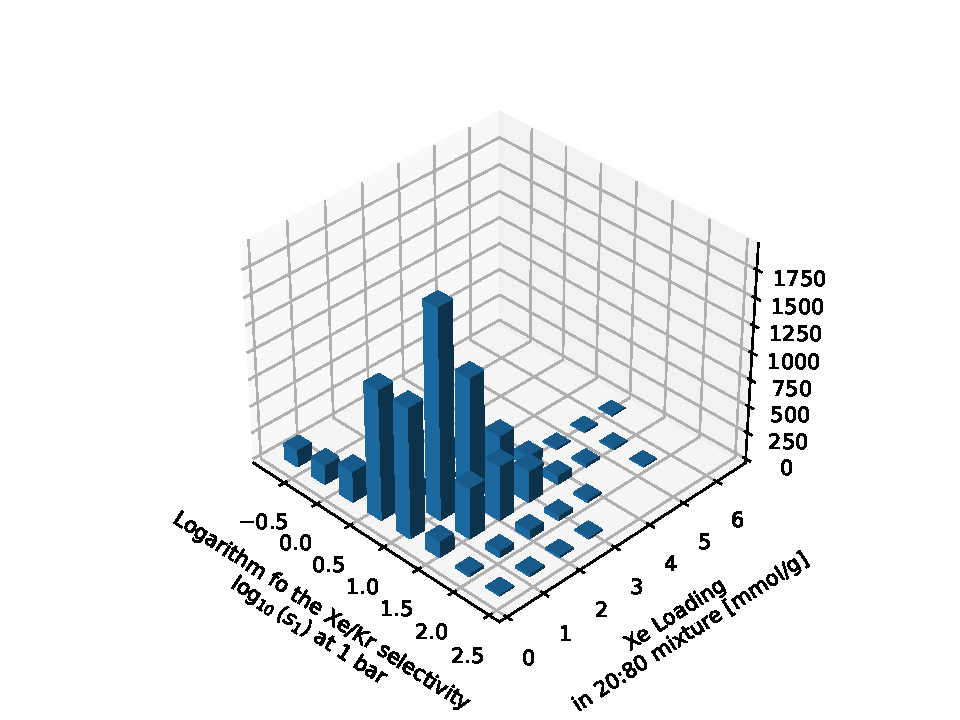
\includegraphics[width=0.48\textwidth]{figures/2-thermo/3D_hist_selec_uptake.pdf}
  \caption{3D histograms of in a bidimensional space formed by the Xe/Kr selectivity and the xenon uptake. The z-axis represents the number of structures with characteristics close to the one specified in x and y-axis. A base 10 logarithm has been applied to the selectivity values.}\label{fgr:3D_uptake}
\end{figure}

Furthermore, even if we know that it is possible to optimize either the xenon uptake or the Xe/Kr selectivity, these very successful materials are very rare inside a given diverse dataset. In the histogram presented in Figure~\ref{fgr:3D_uptake}, the number of very selective materials is very low, same for the high-capacity materials. The most frequent materials have a selectivity between $1$ and $10$ and an uptake below \SI{3}{\mmol\per\gram}. These values can be considered the standard values of nanoporous material for Xe/Kr separation, which sets reference values to compare the various performance metrics and build a chemical intuition. A selectivity above $20$ is therefore considered rather high (even if the top materials have a much higher selectivity\cite{Pei_2022}) and a xenon uptake above \SI{4}{\mmol\per\gram} is also a pretty good adsorption capacity. The rarity of these top-performing materials gives the impression of searching a needle in a haystack, which has prompted some computational studies to design their algorithm to focus on finding the best materials rather than to describe equally all materials.\cite{Deshwal_2021,Glasby_2021} 

\subsubsection{Surface areas}

\begin{figure}[h!]
  \centering
  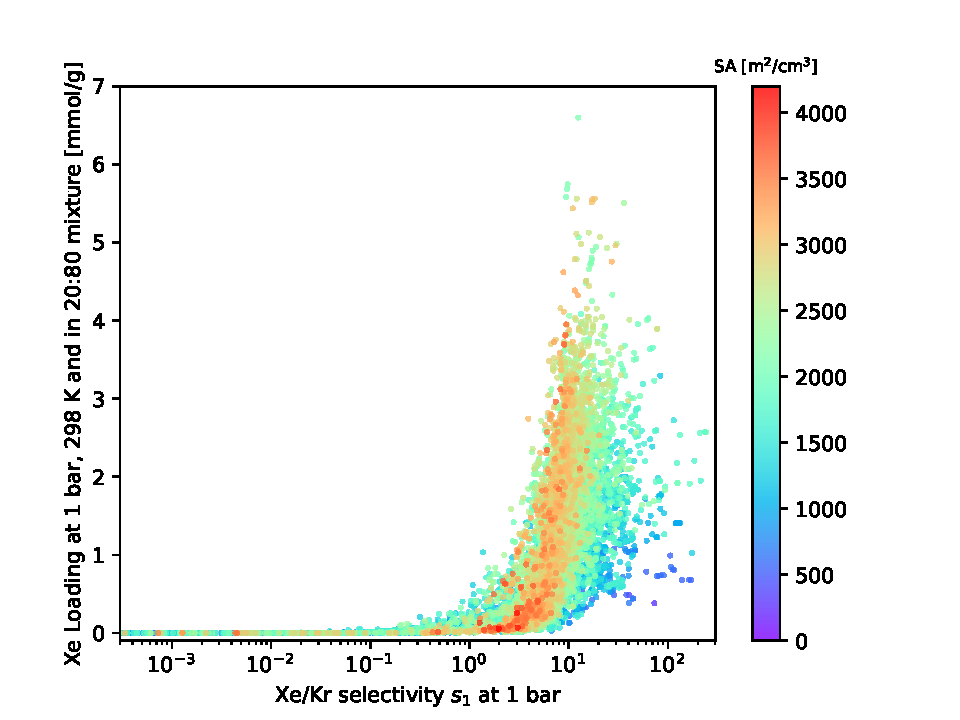
\includegraphics[width=0.48\textwidth]{figures/2-thermo/Scatterplot_uptake_selectivity_sa.pdf}
  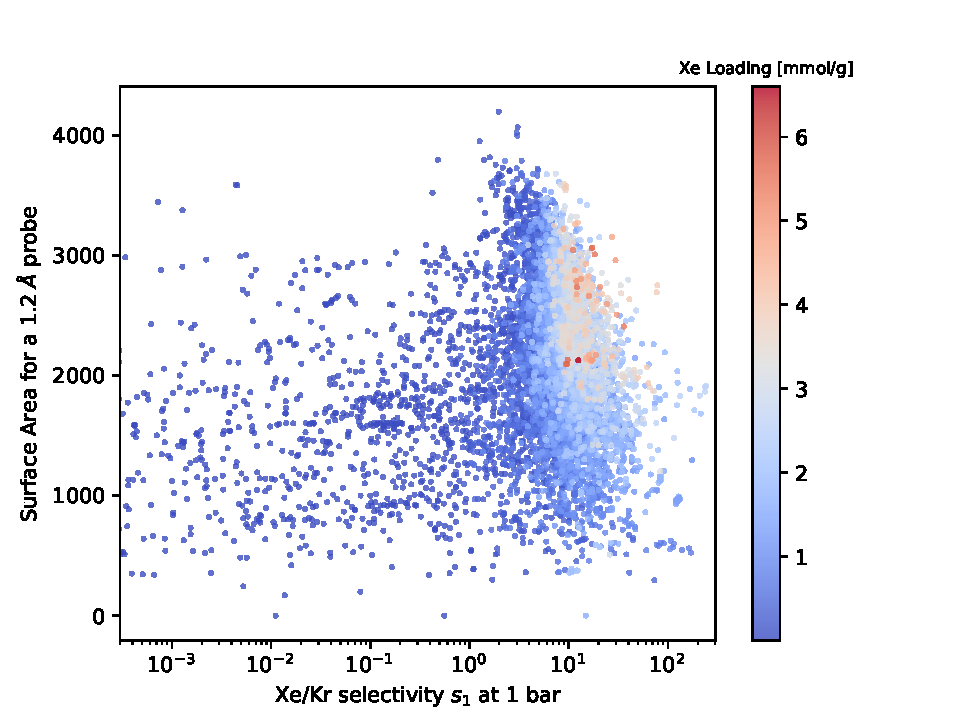
\includegraphics[width=0.48\textwidth]{figures/2-thermo/Scatterplot_sa_selectivity.pdf}
  \caption{On the left: scatterplot of the xenon uptake as a function of the selectivity and labeled by the values of the surface area. On the right: scatterplot of the selectivity and the surface area labeled by the quantity of xenon adsorbed. The selectivity and uptake are calculated by a GCMC simulation of a 20:80 Xe/Kr mixture.}\label{fgr:sa}
\end{figure}

As demonstrated by other studies on methane storage applications by Wilmer et al.\cite{Wilmer_2012} and then later by Fernandez et al.\cite{Fernandez_2013}, the methane uptake is maximal for a specific optimal range of surface area values ($2500$-$3000$~\si{\square\meter\cubic\centi\meter}). Higher values of surface area will not yield to higher values of methane uptake. This limitation also occurs for the selectivity as we can see in the right plot of the Figure~\ref{fgr:sa}. Materials with a selectivity around $5$ will have any surface areas from $0$ to $4000$~\si{\square\meter\cubic\centi\meter}, whereas the ones with a selectivity above $40$ will have a surface area below $2500$~\si{\square\meter\cubic\centi\meter}. The optimal surface area for xenon uptake would on the other hand be between $2000$ and $3000$~\si{\square\meter\cubic\centi\meter}. The relationship between selectivity and surface area is quite complex, we cannot clearly state a precise range of surface areas that guarantees a high selectivity. This structural descriptor cannot characterize the selectivity, it needs to be coupled with other descriptors. 

Looking at the 3D histogram on the Figure~\ref{fgr:3D_hist_sa_vol}, we can see the breakdown of the surface area ranges for different categories of selectivity. For selectivity values higher than $92$, the surface areas are most likely to be under $2000$~\si{\square\meter\cubic\centi\meter}; between $92$ and $35$, there is a slightly wider range that goes to $2500$~\si{\square\meter\cubic\centi\meter}; between $35$ and $13$, the interval goes even further to $3500$~\si{\square\meter\cubic\centi\meter} but is mostly centered between $1000$ and $2500$~\si{\square\meter\cubic\centi\meter}. This split view of the distributions gives a better grasp on what the best materials look like; however the surface area will never be a deterministic variable --- we will never be available to deduce the selectivity by simply looking at the surface area, because a surface area between, for instance, $500$ and $1000$~\si{\square\meter\cubic\centi\meter} have a relatively good chance of being selective but it concerns a lot of materials and it even has a higher chance of having a selectivity between $5$ and $35$ than a selectivity higher than that. 

\begin{figure}[h!]
  \centering
  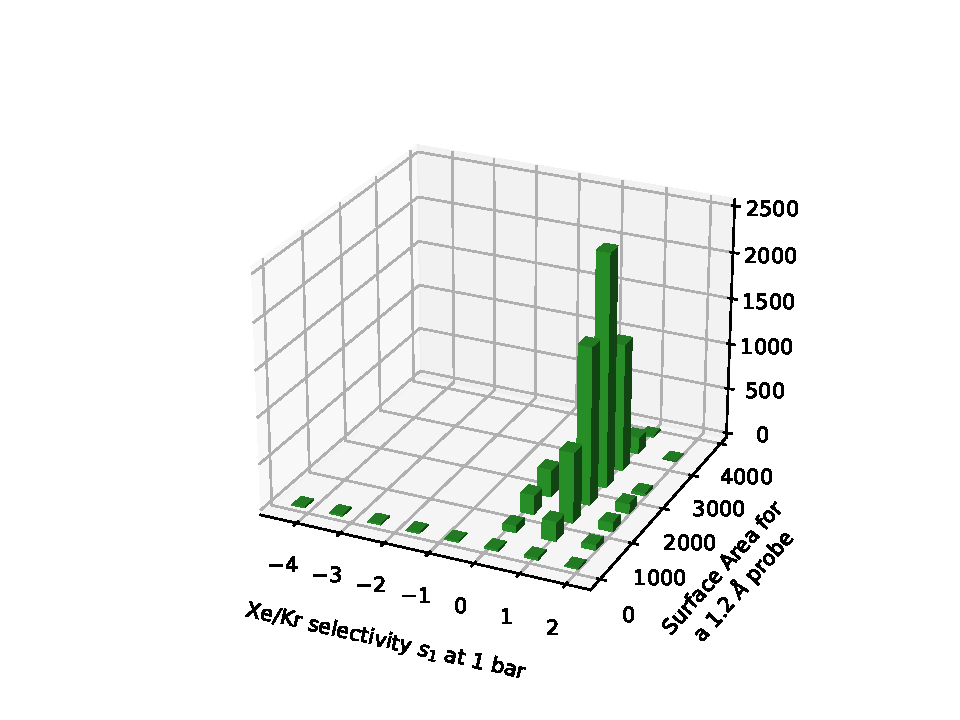
\includegraphics[width=0.48\textwidth]{figures/2-thermo/3D_hist_selec_SA.pdf}
  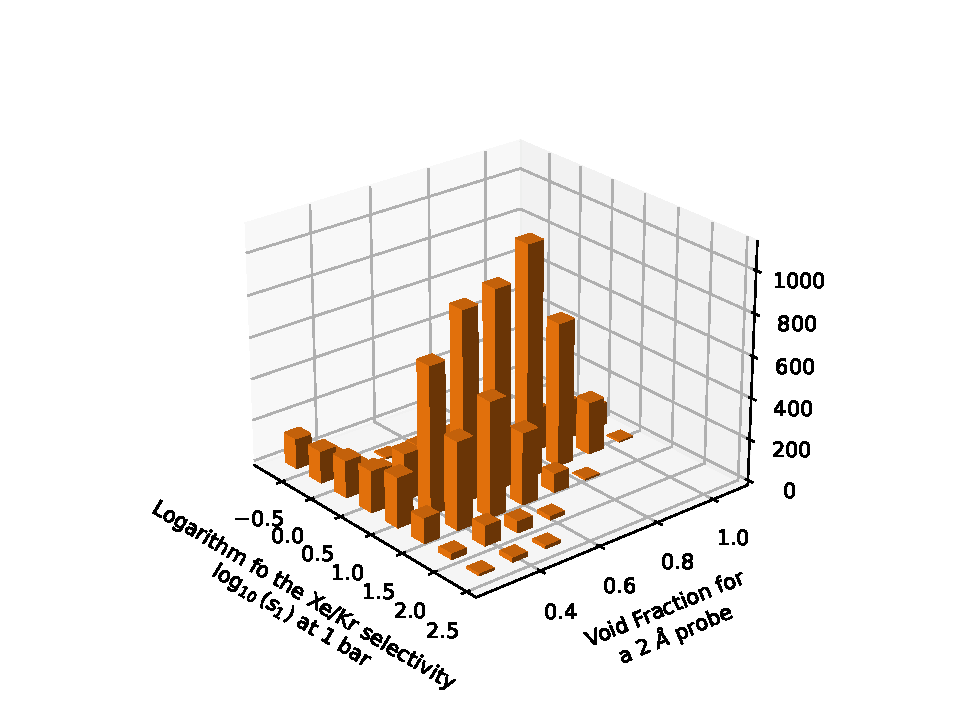
\includegraphics[width=0.48\textwidth]{figures/2-thermo/3D_hist_selec_vol.pdf}
  \caption{3D histograms of in a bidimensional space formed by the Xe/Kr selectivity and the surface areas (on the left) and formed by the Xe/Kr selectivity and the pore void fractions (on the right). A base 10 logarithm has been applied to the selectivity values. Bin size increased by 2.4 (on log scale) for the selectivity, by about $500$~\si{\square\meter\cubic\centi\meter} for the surface areas and by $0.125$ for the void fraction. }\label{fgr:3D_hist_sa_vol}
\end{figure}

\subsubsection{Void fraction}

A similar analysis of the relationship with the void fraction was also carried out by Wilmer et al. (Figure 5 of Ref.~\cite{Wilmer_2012}) and an optimal value of the void fraction was found at around $0.8$. As we can see on the plots of the Figure~\ref{fgr:vol}, the materials with the highest value of Xe uptake have void fraction values around $0.5$, whereas the ones with the highest value of selectivity have much lower void fractions around $0.1$. The optimal range of void fraction for uptake would be between $0.2$ and $0.6$, whereas the one for selectivity is completely dissociated and is below $0.2$. We can characterize a bit more finely the selectivity using the void fraction than using the surface area, even though they both give very similar results. Both descriptors describe a rather dense material with a ``microporosity'', in the sense of the IUPAC\cite{Sing_1985}, which is characterized by medium-low pore volume and surface area.

\begin{figure}[ht]
  \centering
  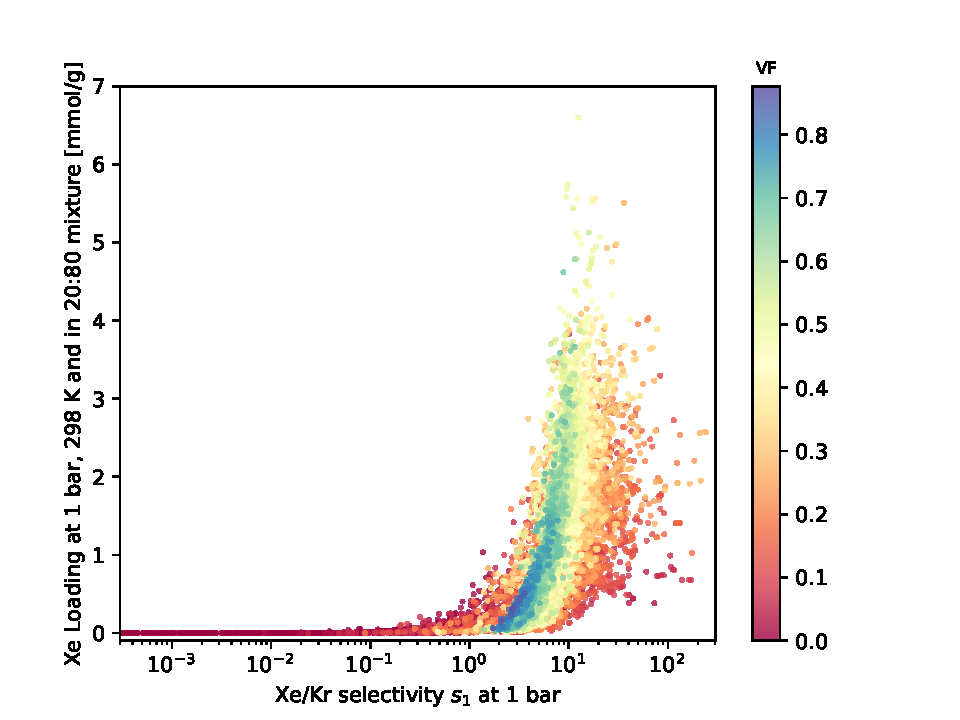
\includegraphics[width=0.48\textwidth]{figures/2-thermo/Scatterplot_uptake_selectivity_vol.pdf}
  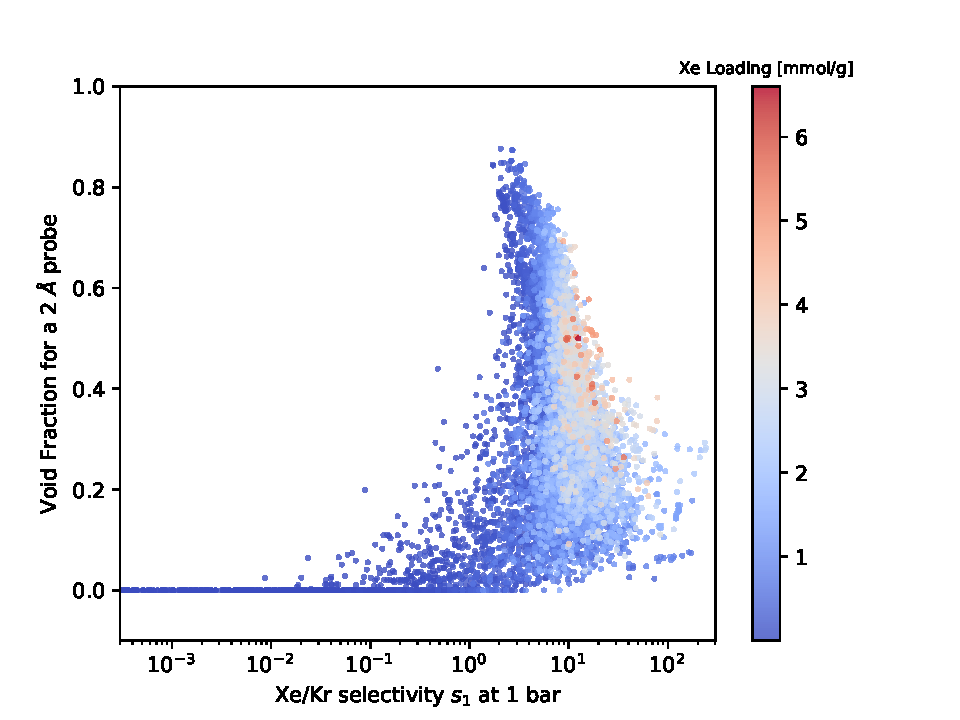
\includegraphics[width=0.48\textwidth]{figures/2-thermo/Scatterplot_vol_selectivity.pdf}
  \caption{On the left: scatterplot of the xenon uptake as a function of the selectivity and labeled by the values of the void fraction. On the right: scatterplot of the selectivity and the void fraction labeled by the quantity of xenon adsorbed. The selectivity and uptake are calculated by a GCMC simulation of a 20:80 Xe/Kr mixture.}\label{fgr:vol}
\end{figure}

By carrying out a similar analysis than for the surface areas bu for the void fraction using the Figure~\ref{fgr:3D_hist_sa_vol} (right), we can also identify different intervals of void fractions that correspond to highly selective materials. For instance, selectivity values above $92$ correspond to materials with a porosity between {$0$\%} and {$37.5$\%} (with a higher peak between {$12.5$\%} and {$25$\%}); selectivity values between $92$ and $35$ can be found in materials with a void fraction between {$0$\%} and {$50.0$\%} and much more frequently found for void fraction between {$12.5$\%} and {$37.5$\%}; selectivity values between $35$ and $13$ can be found in materials with a void fraction between {$0$\%} and {$75.0$\%} in a bell distribution centered around {$31$\%}. This center of distribution shifts toward higher values of the void fraction as lower selectivity values are considered, which suggests that a rather low porosity (below {$25$\%}) is preferable for selectivity performance. However, as we mentioned for surface areas, the void fraction is not a deterministic variable neither, we cannot predict the performance of the material solely based on this descriptor. Let us investigate whether adding another variable like the pore size as a joint variable wan better characterize the material's performance. 

\subsubsection{Pore size or global cavity diameter}

\begin{figure}[h!]
  \centering
  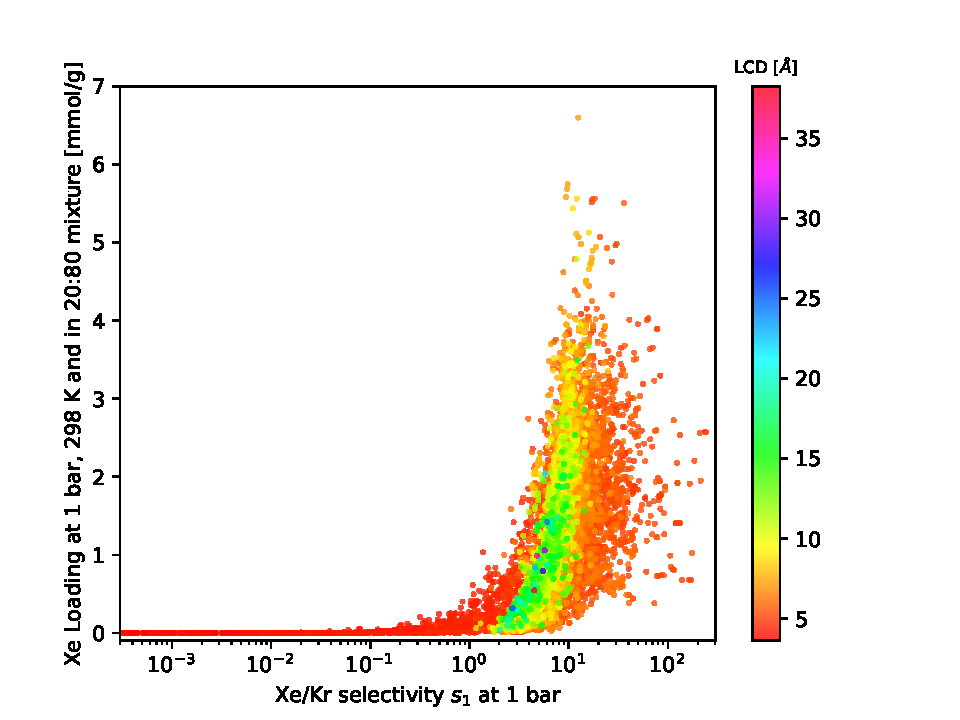
\includegraphics[width=0.48\textwidth]{figures/2-thermo/Scatterplot_uptake_selectivity_gcd.pdf}
  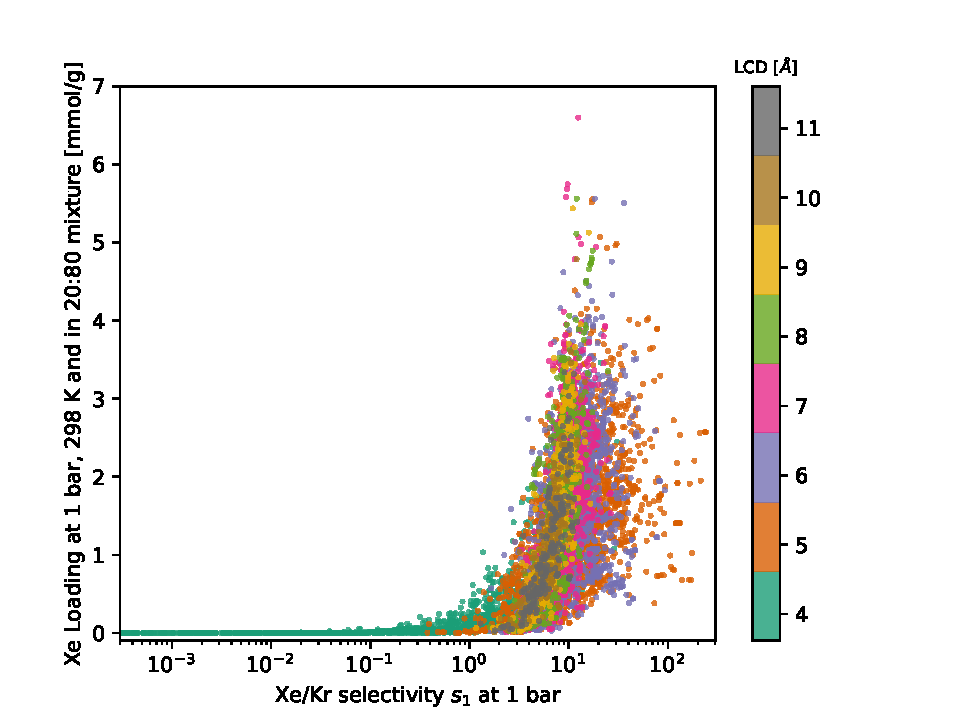
\includegraphics[width=0.48\textwidth]{figures/2-thermo/Scatterplot_uptake_selectivity_gcd_zoom.pdf}
  \caption{Scatterplot of the xenon uptake as a function of the selectivity (20:80) and labeled by the values of the GCD (left). The same scatterplot restricted to values of GCD between ($3.6$ and $11.6$~\si{\angstrom}) and labeled using a different color code to distinguish the most selective materials from the least selective ones. The most selective materials are colored in orange corresponding to a pore size adapted for xenon adsorption (around $5$~\si{\angstrom}). The least selective ones are in green, with a pore lower than the size of a xenon hence preventing its adsorption.}\label{fgr:vol}
\end{figure}

If we now look at the joint effects of the void fraction and the global cavity diameter (GCD) on the selectivity, we can note that the most selective materials are located in a very particular domain of this bidimensional descriptor space. On Figure~\ref{fgr:gcd_vf}, the structures with a selectivity over $10$ are very likely to have a void fraction under $0.4$ with a rather wide range of GCD. However, as we can see on the filtered version of the plot (on the right), the most selective materials (over $40$) exist, on the other hand, in a very narrow range of GCD values between $4.8$ and $6$~\si{\angstrom} approximately. This can be explained by the size of a xenon atom being very close to these GCD values, which allows a maximal stabilization of the xenon that we want to separate from krypton. The krypton being slightly smaller, the interaction with the pores are less favorable, hence explaining the higher selectivity we observe. 

\begin{figure}[h!]
  \centering
  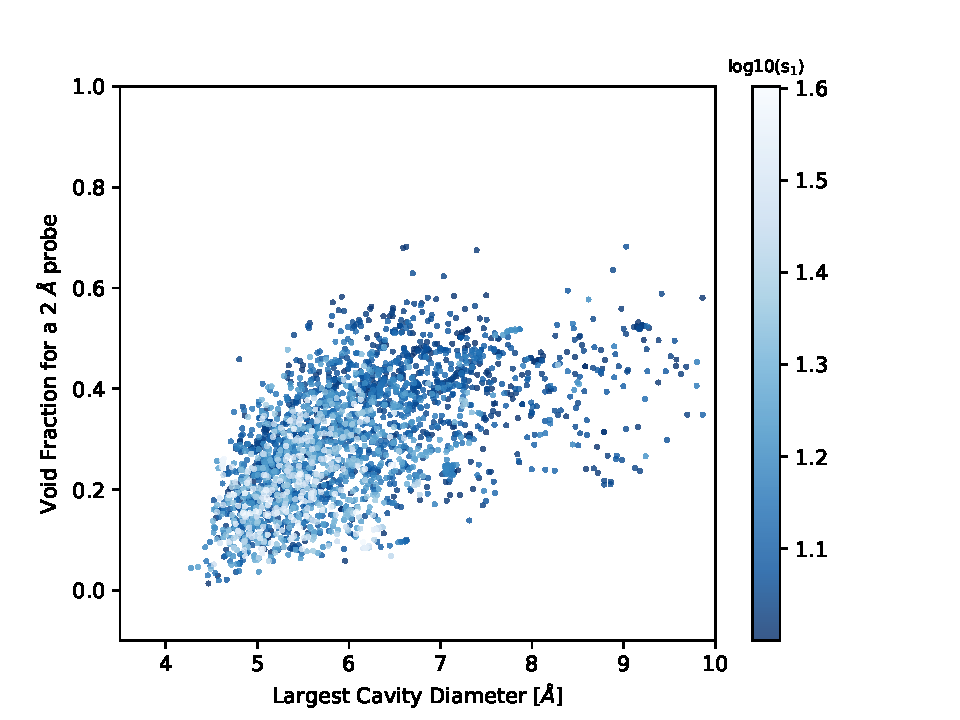
\includegraphics[width=0.48\textwidth]{figures/2-thermo/Scatterplot_vf_gcd_selectivity.pdf}
  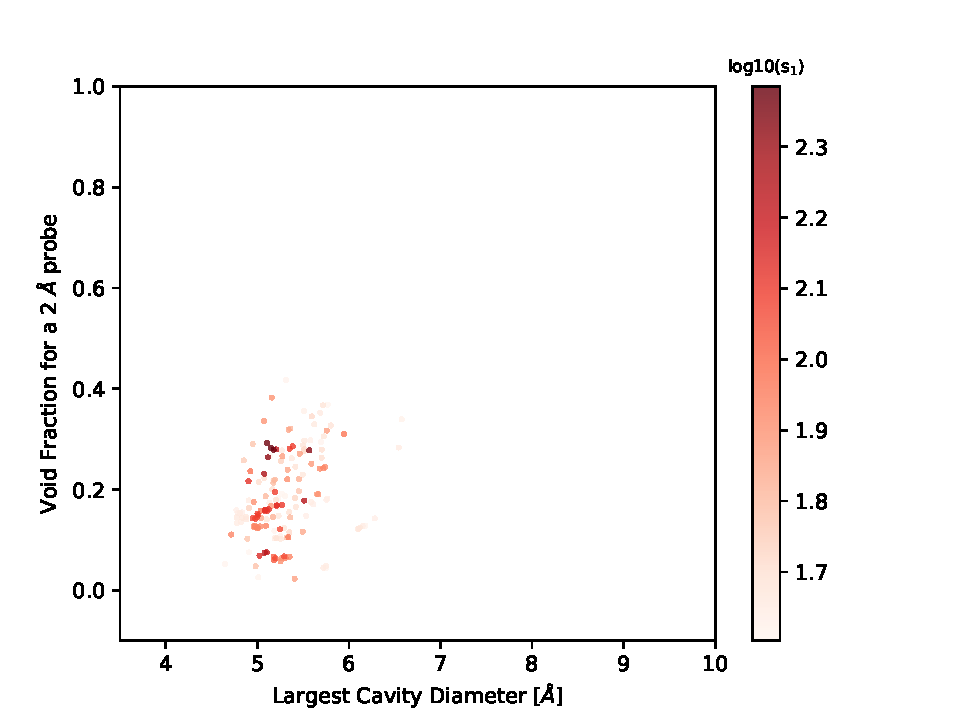
\includegraphics[width=0.48\textwidth]{figures/2-thermo/Scatterplot_vf_gcd_selectivity_zoom.pdf}  
  \caption{Scatterplots of the void fraction as a function of the GCD and labeled by the log$_10$ of the selectivity values. On the left, only the materials with a selectivity between $10$ and $40$ are considered; and on the right, selectivity values over $40$.}\label{fgr:gcd_vf}
\end{figure}


As presented in the previous chapter, Simon et al.\ found that the most selective materials have a pseudo-spherical shape with a size close to the diameter of a xenon which is rather dense and not very porous. By taking a slightly different approach and including the xenon uptake as a co-metric alongside the selectivity, we found very similar results by identifying specific intervals of the cavity diameter and the pore volume. However, this structure--property relationship can only be used as a description of selective materials, and no prediction could be achieved by only using structural descriptors. 

\subsubsection{Effect of the composition}

Finally, we previously only tackled one type of composition (20:80) associated to the extraction of xenon and krypton from a cryogenic distillation from the air (see section 1.3.1). We are now going to investigate the effects of the composition by looking at the case of xenon/krypton separation in spent nuclear fuel off-gases. In nuclear applications, the mixture has a 90:10 Xe/Kr ratio, which is much richer in xenon in comparison to the previous one. For this reason, the quantity of xenon adsorbed in the materials will mechanically be higher than previously. However, the second quotient in the formula of selectivity in equation~\ref{eq:selec} compensates the first one that will be logically higher. Here, we want to evaluate these two effects to see if they cancel each other out or there are different trends depending on the composition value. 

As shown on the Figure~\ref{fgr:SI:overview_2080_9010}, selectivity values of both compositions are quite close. However, we can note a slight decrease in performance when increasing the proportion of xenon in the mixture for some materials that are moderately selective ($s$ between $2$ and $50$). This loss in performance could be explained by the fact that the materials display pores with different xenon affinities. With a lower proportion of xenon, the Xe adsorbates would access preferentially the most favorable pores and the small quantity of xenon is concentrated there. Whereas when there is a higher content of xenon, these most favorable sites begin to saturate and the xenon need to compete with krypton in much less favorable sites hence decreasing slightly the selectivity. We will see that later, we could use very similar reasoning to explain another variable that could change the selectivity.

\begin{figure*}[ht]
  \centering
    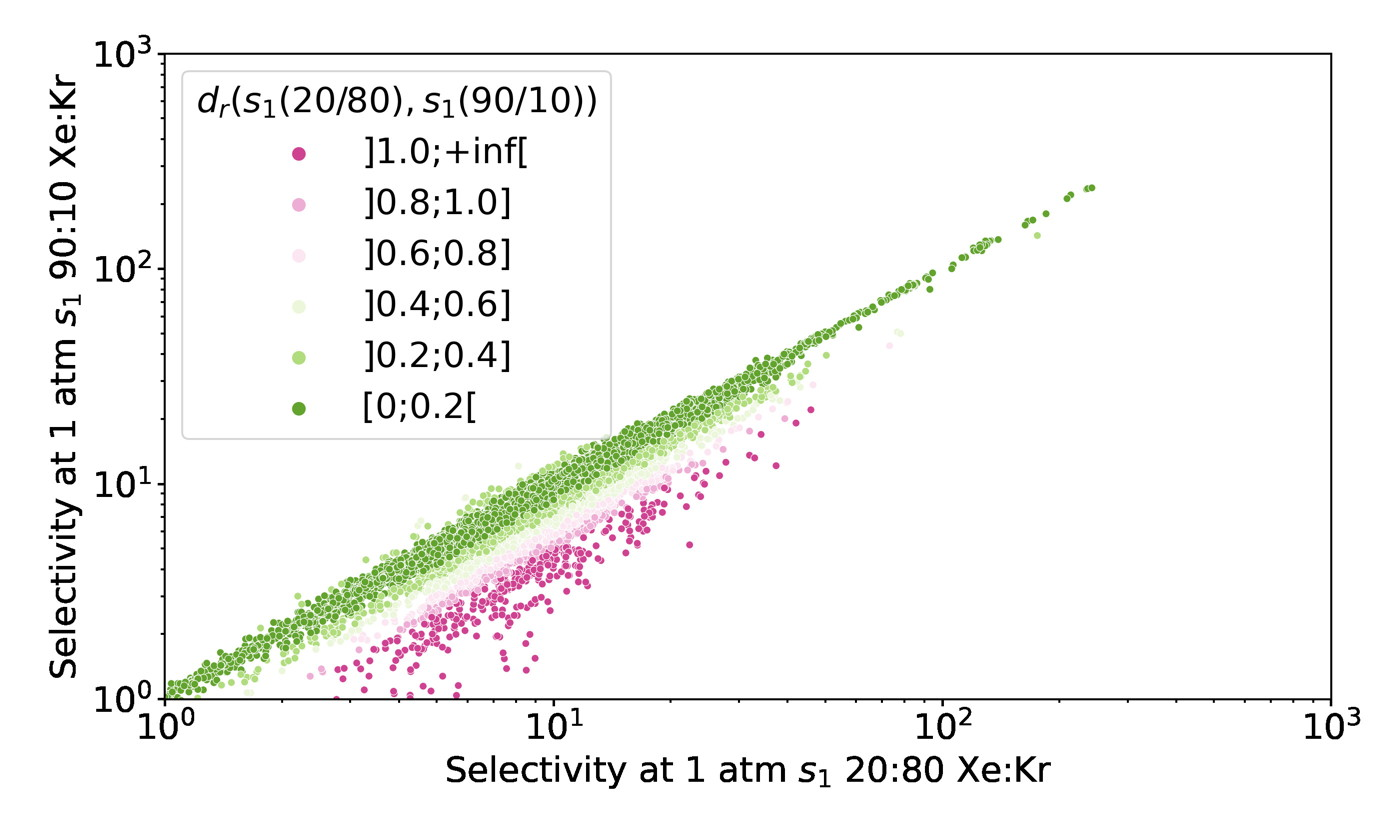
\includegraphics[width=0.45\textwidth]{figures/2-thermo/s_2080_vs_s_9010_overview_log.jpg}
    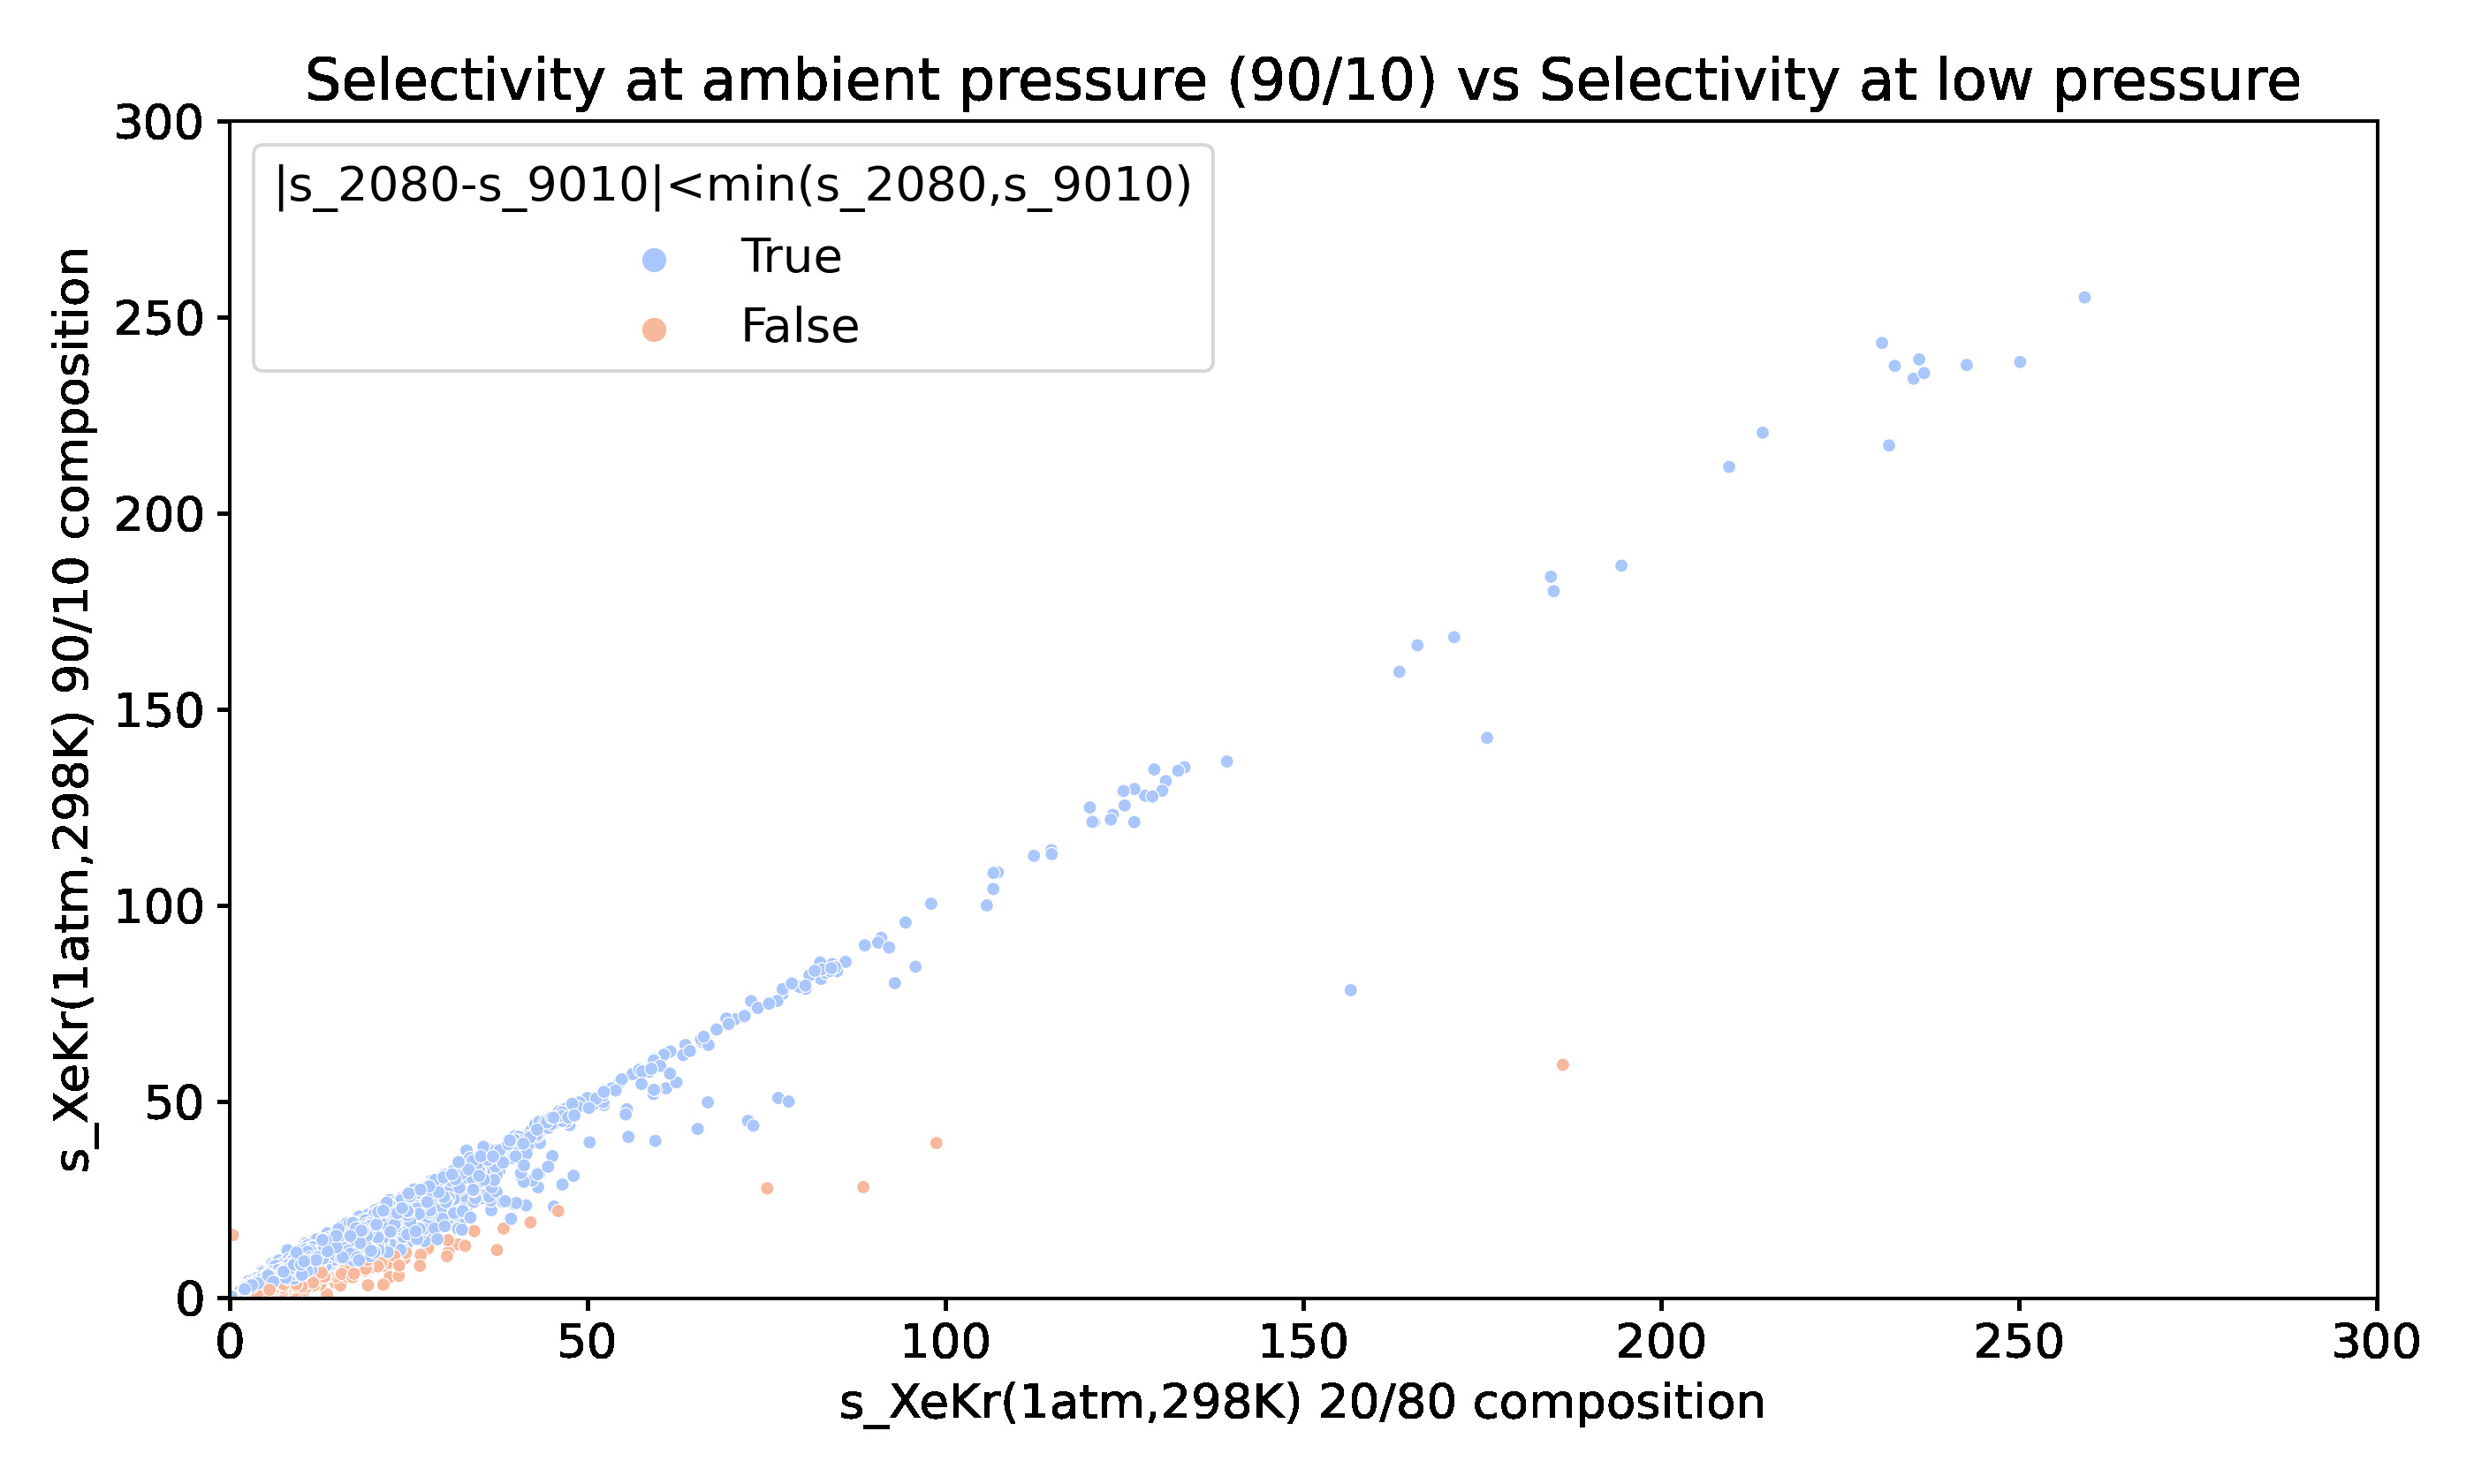
\includegraphics[width=0.45\textwidth]{figures/2-thermo/s_2080_vs_s_9010_overview.jpg}
    \caption{Illustration (scatterplot) of the difference of selectivity ($s\e{1}(20:80)$ and $s\e{1}(90:10)$) for two different Xe/Kr mixture compositions 20:80 (x-axis) and 90:10 (y-axis) at \SI{1}{\atm} and \SI{298}{\kelvin}. On the left, the axis is in log scale and the relative difference of selectivity between the two compositions is particularly high for the points labeled in purple. On the right, the axis is in linear scale and we only label the point to differentiate the materials with relative difference under and over $1$.}
    \label{fgr:SI:overview_2080_9010}
  \end{figure*}

%higher uptakes
We will now see the effect of the composition on the different analysis we carried out on the different structural descriptors. One of the major changes when considering a mixture with much more xenon is the values of the xenon uptake. The nanopores of selective materials ($1<s_1\leq 50$) are much more saturated in Xe and the maximum amount of xenon is therefore much higher. By comparing the Figures~\ref{fgr:vol} and \ref{fgr:compo}, the maximum uptake is now \SI{11.7}{\milli\mole\per\gram} instead of \SI{6.6}{\milli\mole\per\gram} (for the 20:80 composition). For moderately selective materials, at 20:80, the xenon competes with krypton mainly in the most selective nanopores, but when we increase the xenon content it has to compete with krypton in much less favorable sites since the other sites are already saturated. We previously stated that the most selective ($s_1>50$) materials could reach up to \SI{4.0}{\milli\mole\per\gram} of xenon uptake, for a composition with a higher xenon content, and it reaches up to \SI{4.2}{\milli\mole\per\gram} again, which is not a big change. For the most selective materials, the previous conclusion on the maximum uptake can still stand. Because of the extremely high selectivity, the change in composition does not change the nature of the adsorbed state and about the same quantities of xenon are present in the pores. Finally, we can say that a higher content in xenon does not influence a lot the most selective materials' performance but it could alter the selectivity and increase a lot the xenon uptake for some moderately selective materials.

\begin{figure}[h!]
  \centering
  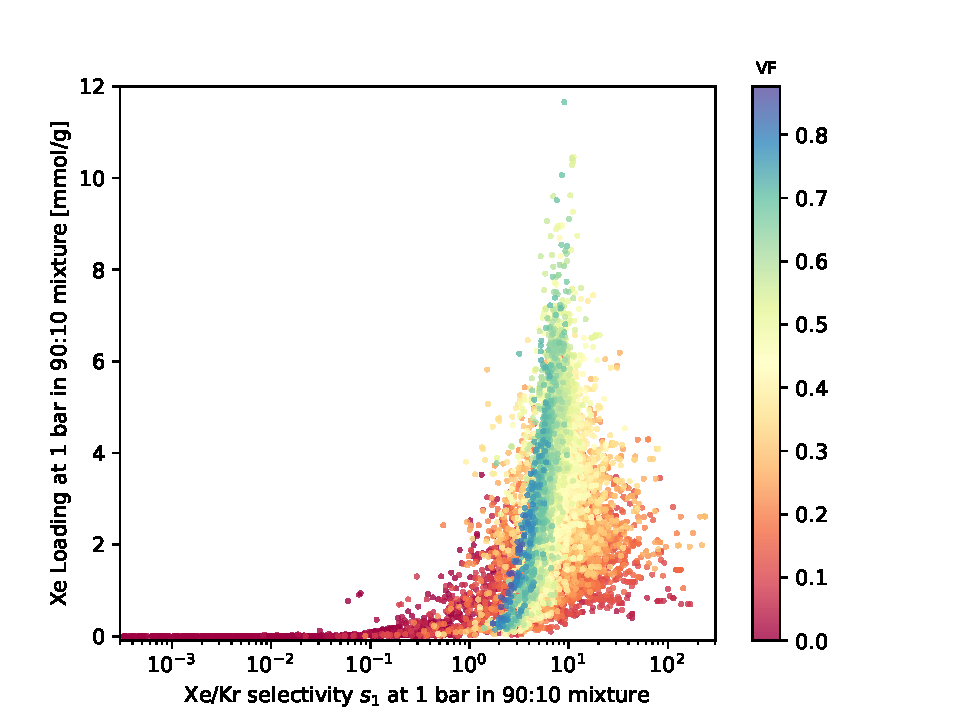
\includegraphics[width=0.48\textwidth]{figures/2-thermo/Scatterplot_uptake_selectivity_vol_9010.pdf}  
  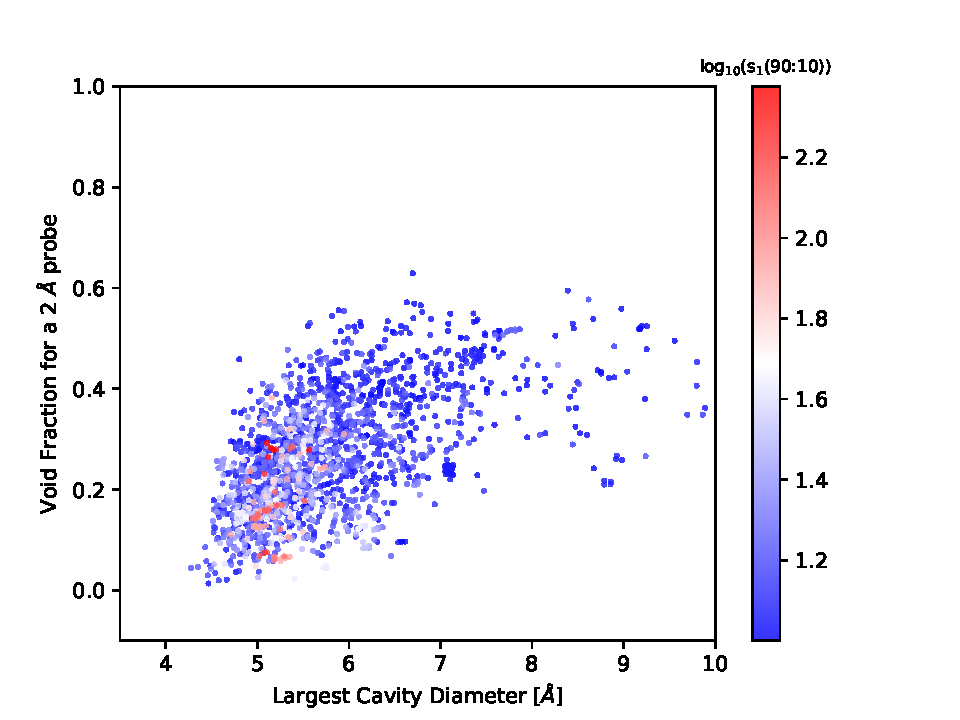
\includegraphics[width=0.48\textwidth]{figures/2-thermo/Scatterplot_vf_gcd_selectivity9010.pdf}
  \caption{Illustration of the effect of the composition by representing the same figures as in \ref{fgr:vol} and \ref{fgr:compo} but for a 90:10 composition. On the left: scatterplot of the xenon uptake as a function of the selectivity ($s\e{1}(90:10)$) and labeled by the values of the void fraction. On the right: scatterplots of the void fraction as a function of the GCD and labeled by the selectivity ($s\e{1}(90:10)$) values superior to $10$ in log-scale.
  Distribution GCD / VF . $s>10$ puis $s>40$}\label{fgr:compo}
\end{figure}

Finally, the composition does not affect the previously determined structural characteristics that a material needs to be very selective. As we can see on the right plot of the Figure~\ref{fgr:compo} (right), the most selective materials still have pore size around \SI{5}{\angstrom} and porosity under {$40$\%}. This structural domain constitutes a necessary condition a selective material should have but being in this domain is not enough since less selective materials can also display these characteristics. Now that we described the geometrical conditions needed to have a good selectivity, we will focus on the thermodynamic origins of the selectivity by focusing on energy-based quantities and the different correlations between them.

\subsection{Thermodynamic quantities correlations}

In this section, our goal is not directly to address the structure--property relationships, but rather to map out the details of the thermodynamic features of Xe/Kr adsorption and separation in nanoporous materials. We used the high-throughput screening methodology as a way to map out the space of thermodynamic properties, going beyond the usual quantities of selectivity and uptake, to focus more specifically on the role of adsorption enthalpy and entropy, the differences between Xe and Kr adsorption thermodynamics, and between selectivity at low and high pressure.

To evaluate the performance of a given nanoporous material for separation in the low loading (or low pressure) limit, Henry's constants are often calculated from linear fits of low-pressure adsorption isotherm data --- both experimentally and computationally. In this section, we investigate the thermodynamics of Xe and Kr adsorption at low pressure. Here, we have calculated the low-pressure adsorption properties by using the Widom insertion method\cite{Widom1963, frenkel2001widom} on 9,668 structures from the dataset selected. It has higher accuracy than the fitting of isotherms, where it can be difficult to know what the extent of the linear adsorption regime is. With these simulations, we could obtain for each material the Henry's constant $K$ and the adsorption enthalpy $\Delta\e{ads}H\e{0}$ (at the zero loading limit) for both xenon and krypton. The Xe/Kr thermodynamic selectivity $s\e{0}$ in the low-pressure limit is then determined by the ratio $s\e{0} = K\ex{Xe}/K\ex{Kr}$ of the Henry's constants for the two gases. In the following, we look at the statistical relationships between the thermodynamic quantities at low pressure: $s\e{0}$, $K\ex{Xe}$, $K\ex{Kr}$, $\Delta\e{ads}H\e{0}\ex{Xe}$, $\Delta\e{ads}H\e{0}\ex{Kr}$ and $\Delta\e{exc}H\e{0}$.


\begin{figure}[t]
\centering
  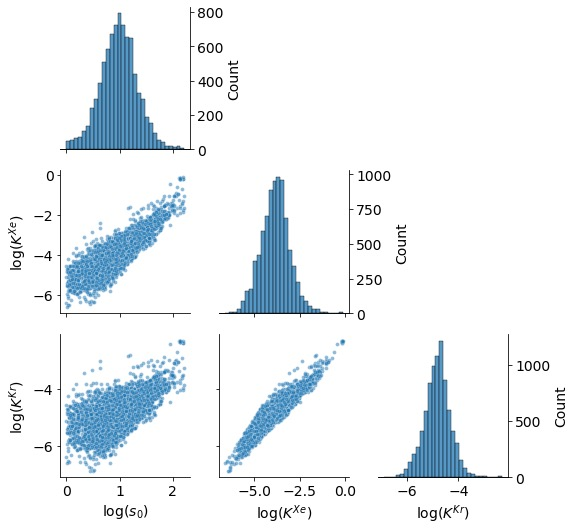
\includegraphics[width=0.6\linewidth]{figures/2-thermo/Henry_0.jpg}
  \caption{For 8,401 MOFs with favorable thermodynamic Xe/Kr selectivity ($s\e{0} > 1$), pair plots of $\log\e{10}(s\e{0})$, $\log\e{10}(K\ex{Xe})$ and $\log\e{10}(K\ex{Kr})$ (the Henry's constants are in~\si{\milli\mol\per\gram\per\pascal}) in the off-diagonal subplots (note that the y-axis is displayed on the right side) and the distribution of each quantity are on the diagonal (note that the y-axis displayed on the right side corresponds to the count and the x-axis is correctly labeled below each subplot).}
  \label{fgr:histo_K}
\end{figure}


We display the distribution of thermodynamic properties of materials with favorable thermodynamic Xe/Kr selectivity ($s\e{0} > 1$) in Figure~\ref{fgr:histo_K} --- we restrict these plots to selectivity above 1, because those are the materials of interest for separation, and doing so removes several outliers with specific geometries or binding sites (but does not change the overall conclusions). We can first see that although the logarithm of the Xe Henry's constant $K\ex{Xe}$ is weakly correlated to the logarithm of the selectivity $s\e{0}$, this correlation is stronger for highly selective materials. Therefore, in a multistep screening study to identify the most selective materials, it could be possible to use as a ``first filter'' criterion based purely on Xe adsorption, discarding materials below a certain threshold (e.g., the materials with $s_0\ge30$ are contained in the subset with $K\ex{Xe}\ge2.7\,10^{-1}$~\si{\milli\mol\per\gram\per\pascal}). The correlation between $K\ex{Kr}$ and $s\e{0}$, on the other hand, is weaker.

With regard to Henry's constants, we observe a broad selection of behavior, with $K\ex{Xe}$ ranging from $2.6\,10^{-7}$ to $7.9\,10^{-1}$~\si{\milli\mol\per\gram\per\pascal}, and $K\ex{Kr}$ ranging from $1.3\,10^{-7}$ to $5.1\,10^{-3}$~\si{\milli\mol\per\gram\per\pascal}. We also see that statistically, a high affinity for xenon usually translates into a high (relative) affinity for krypton, which is a general trend for noble gases where the adsorption sites are not strongly specific. In order to look more in detail into the thermodynamics behind this wide diversity in behavior, we plot in Figure~\ref{fgr:histo_H} the enthalpies involved.

\begin{figure}[t]
\centering
  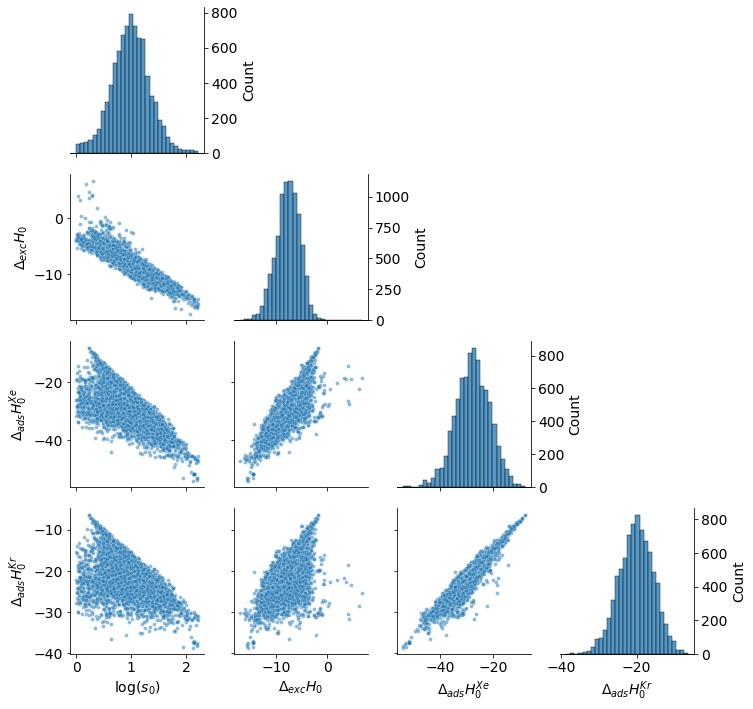
\includegraphics[width=0.7\linewidth]{figures/2-thermo/Enthalpy_0_log.jpg}
  \caption{For 8,401 MOFs with favorable thermodynamic Xe/Kr selectivity ($s\e{0} > 1$), pair plots of $\log(s\e{0})$, $\Delta\e{exc}H\e{0}$, $\Delta\e{ads}H\ex{Xe}\e{0}$ and $\Delta\e{ads}H\ex{Kr}\e{0}$ (the enthalpies are in~\si{\kilo\joule\per\mol}) in the off-diagonal subplots and the distribution of each quantity is on the diagonal.}
  \label{fgr:histo_H}
\end{figure}

We first observe that the low-loading adsorption enthalpy of xenon ($\Delta\e{ads}H\ex{Xe}\e{0}$) is strongly correlated to that of krypton ($\Delta\e{ads}H\ex{Kr}\e{0}$). Echoing the similar correlation seen between respective Henry's constants, it suggests a rather generic physisorption mechanism is at play in the majority of materials, and that host--adsorbate affinities are mainly determined by the enthalpy. The main driver of Xe/Kr selectivity is neither the xenon nor krypton adsorption enthalpy alone (both are weakly correlated to the selectivity), but as expected their difference, $\Delta\e{exc}H\e{0}$, which is strongly correlated to $\log(s\e{0})$. This is further confirmed by the lack of correlation between selectivity and adsorption entropies (\emph{c.f.} Figure~\ref{fgr:SI:HS_0_log}): the separation is mostly enthalpic in nature, and the entropy causes the dispersion in the correlation between selectivity $\log(s\e{0})$ and $\Delta\e{exc}H\e{0}$.

\begin{figure*}[h]
  \centering
    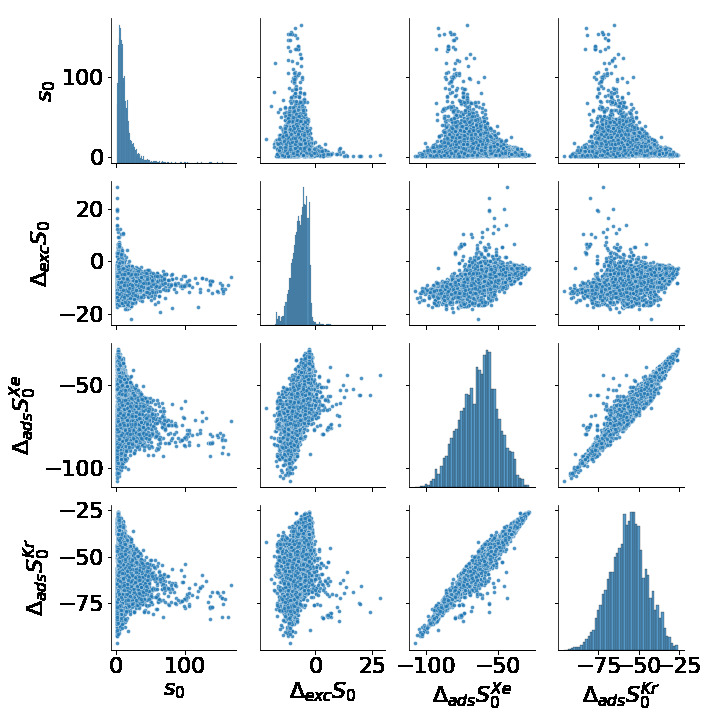
\includegraphics[width=0.60\textwidth]{figures/2-thermo/Entropy_0.jpg}
    \caption{For 8,401 MOFs with favorable thermodynamic Xe/Kr selectivity ($s\e{0} > 1$), pair plots of $s\e{0}$, $\Delta\e{exc}S\e{0}$, $\Delta\e{ads}S\ex{Xe}\e{0}$ and $\Delta\e{ads}S\ex{Kr}\e{0}$ in the off-diagonal subplots and the distribution of each quantity are on the diagonal.}
    \label{fgr:SI:HS_0_log}
\end{figure*}

Analyzing the Figure~\ref{fgr:SI:HS_0_log} in more detail, the adsorption entropy of xenon and krypton being noticeably correlated, their difference (the exchange entropy) does not have a lot of variations (see Figure~\ref{fgr:SI:dist0}) compared to the enthalpy. This thermodynamic quantity plays a minor role in the selectivity performance of the materials. However it seems that the most selective materials do not have any values of exchange entropy but is centered around a value of about \SI{-10}{\kilo\joule\per\mole\per\kelvin}. This is not a clean correlation but rather a necessary attribute of a selective material.

\begin{figure*}[h]
  \centering
    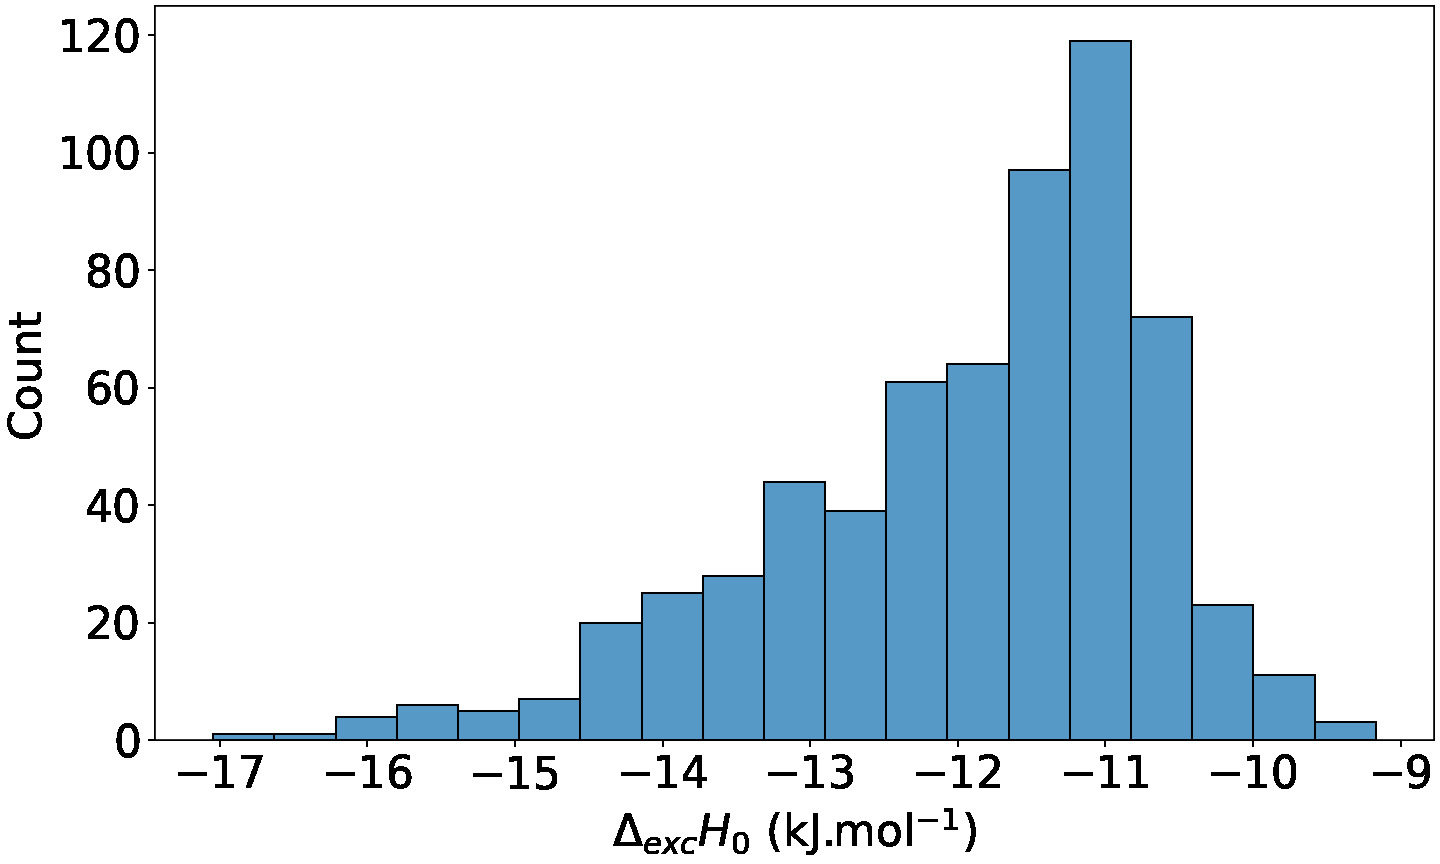
\includegraphics[width=0.45\textwidth]{figures/2-thermo/Delta_H_0.jpg}
    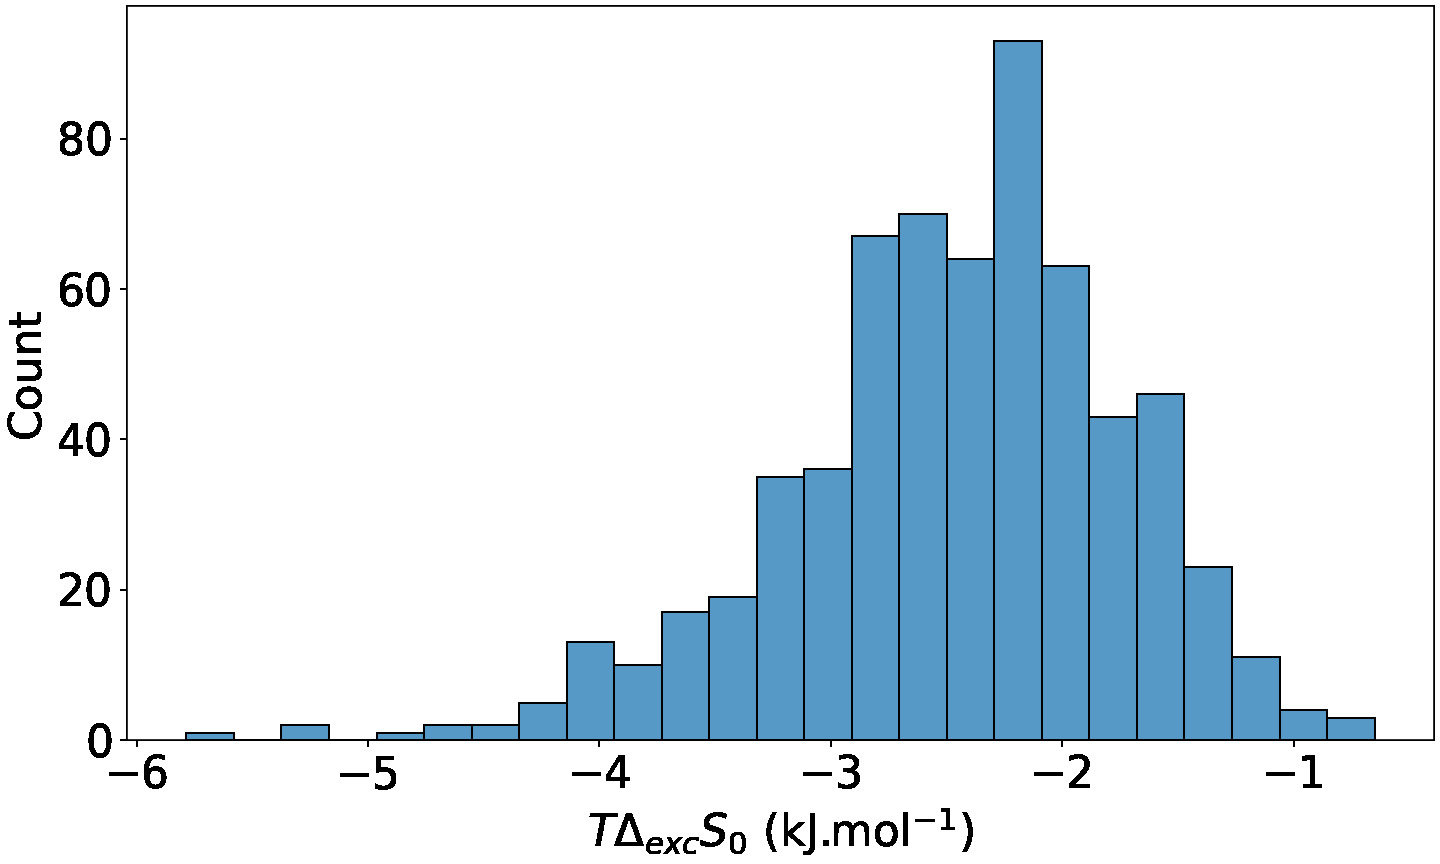
\includegraphics[width=0.45\textwidth]{figures/2-thermo/T_Delta_S_0.jpg}
    \caption{Distribution of the enthalpy $\Delta\e{exc}H\e{0}$ and entropy $T\Delta\e{exc}S\e{0}$ of exchange at low pressure on the 630 most selective structures}
    \label{fgr:SI:dist0}
\end{figure*}

To emphasize one more time on the enthalpic nature of the separation by comparing the base 10 logarithm of the Henry constant (proportional to the adsorption free energy) and the adsorption enthalpy for both xenon and krypton. We can see, Figure~\ref{fgr:SI:HK} that the free energy can be almost totally explained by the enthalpy, which confirms the secondary role of the entropy that explains the variance in this linear relation. The effect of the entropy makes the correlation quite weak for the less favorable adsorption materials, but as we move to more negative values of the adsorption enthalpies, the correlation is stronger and stronger. The most selective materials have an almost negligible entropic contribution in the final free energy value ($G=H-TS$).

\begin{figure*}[h]
  \centering
    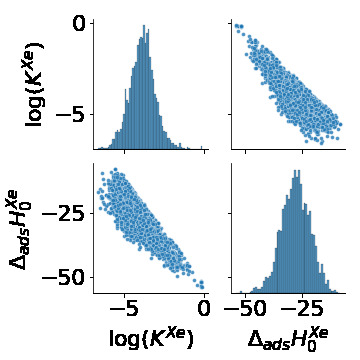
\includegraphics[width=0.35\textwidth]{figures/2-thermo/H_K_Xe.jpg}
    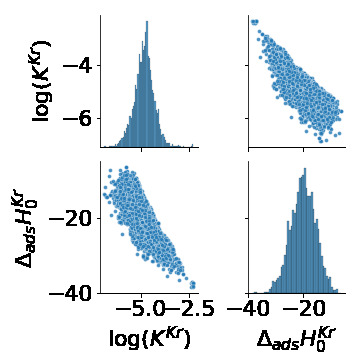
\includegraphics[width=0.35\textwidth]{figures/2-thermo/H_K_Kr.jpg}
    \caption{For 8,401 MOFs with favorable thermodynamic Xe/Kr selectivity ($s\e{0} > 1$), pair plots of $\log(K\e{H}\ex{i})$ and $\Delta\e{ads}H\ex{i}\e{0}$ in the off-diagonal subplots for both i$=$Xe and i$=$Kr and the distribution of each quantity are on the diagonal.}
    \label{fgr:SI:HK}
\end{figure*}

The takeaway messages of this section are based on two relations. The first one is between the Henry constant of xenon and the selectivity: knowing the performance of xenon we can infer the Xe/Kr selectivity --- the most selective materials have very high xenon affinity. The second one concerns the relation between enthalpy and selectivity --- the separation process has an enthalpic nature as a first-order approximation, which is even more true for the most selective materials. By studying the energy interactions within the material, we can understand most of the performance of it. We only looked at the thermodynamic properties at infinite dilution, in the next section we will focus on the effect of the pressure in the selectivity by focusing on a 20:80 Xe/Kr mixture at \SI{1}{\atm} and \SI{298}{\kelvin}. 

%%%%

\section{Selectivity drop}

\subsection{Thermodynamic origins}\label{section:pressure}

\begin{figure}[t]
  \centering
    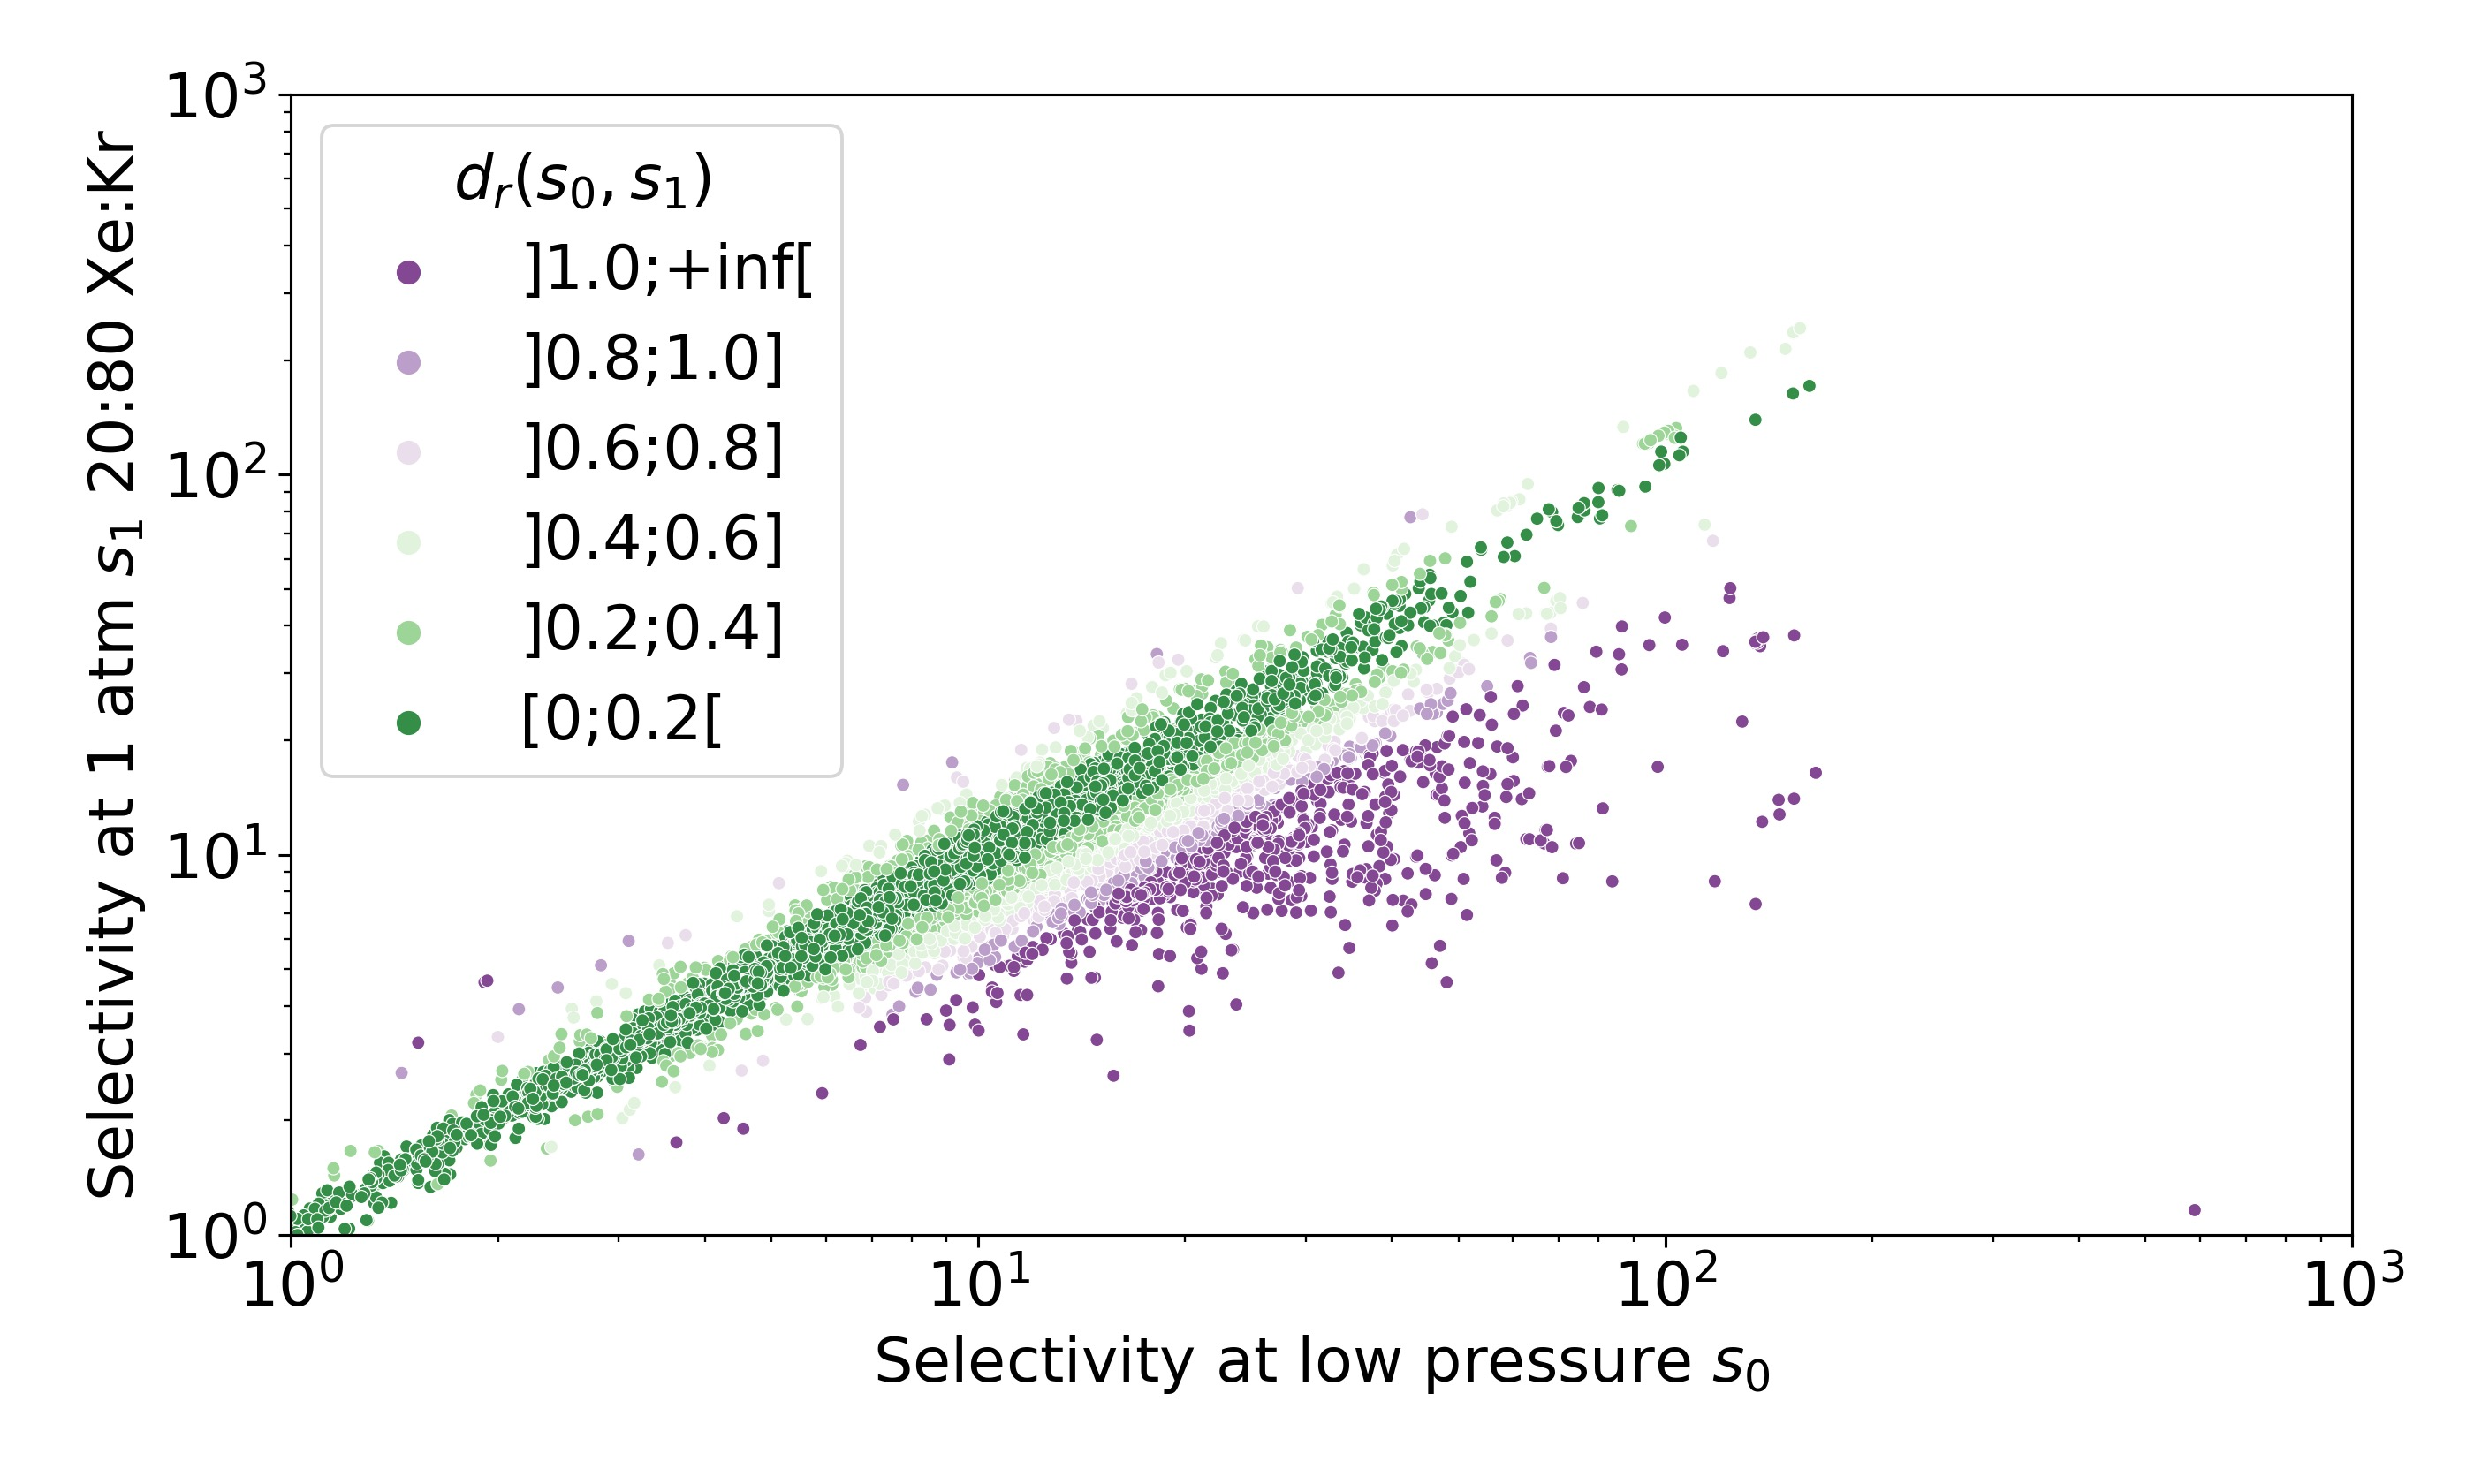
\includegraphics[width=0.6\linewidth]{figures/2-thermo/s_0_vs_s_2080_overview_log.jpg}
    \caption{Difference of selectivity between low pressure and at a \SI{1013}{\hecto\pascal} pressure for a 20:80 xenon krypton composition. The relative difference between the low-pressure selectivity and the ambient pressure is particularly high for the points labeled in purple.}
    \label{fgr:overview}
\end{figure}

In this section we focus on the impact of a change of working pressure on the adsorption selectivity, and analyze its thermodynamic origins. This is key to accurately assess the thermodynamics of adsorption in different working conditions for specific industrial processes, and any insight into the impact of pressure on selectivity may allow for faster screening limited at selected thermodynamic conditions.

We calculated the selectivity $s\e{1}$ at pressure $1$~atm and ambient temperature using GCMC calculations on the entire dataset, with Xe/Kr mixture composition of 20:80 (found in a byproduct stream from air separation\cite{kerry2007industrial}) and 90:10 (found in the off-gas streams from nuclear waste\cite{auerbach2003handbook}). For high-selectivity materials, we find that the impact of composition appears rather marginal (\emph{c.f.} Figure~\ref{fgr:SI:overview_2080_9010}). In the following, we discuss the selectivity for the 20:80 mixture, which is the most commonly studied one in the literature. To measure the difference in selectivity between low and ambient pressures, we consider a relative difference $d_r(s\e{0},s\e{1})$ defined in equation~\ref{eqn:reldiff}.

\begin{equation} \label{eqn:reldiff}
    d_r(s\e{0},s\e{1}) = \dfrac{\lvert s\e{0} - s\e{1} \rvert}{\min(s\e{0},s\e{1})}
\end{equation}

In Figure~\ref{fgr:overview}, the selectivity at ambient pressure $s\e{1}$ is plotted against its low-pressure counterpart $s\e{0}$ (for materials where $s\e{0} > 1$, as before). The points are color-coded according to the value of $d_r(s\e{0},s\e{1})$, in 6 discrete categories for the sake of clarity. There is some broad level of correlation, see near the diagonal with {61.5\%} of materials where the difference is below {20\%} (near the $s_0 = s_1$ line). We also see clearly that there are many more points ({74.3\%} among the materials with $d_r(s\e{0},s\e{1})\ge 0.2$) below the first bisector ($s_1 < s_0$) than above: for these materials the selectivity $s\e{1}$ at 1~atm is significantly lower than the one at low pressure $s\e{0}$.

This drop in selectivity mainly concerns the materials with a relatively high selectivity $s\e{0} > 10$ (see Figure~\ref{fgr:overview}), and forewarns that considering solely pure-component Henry's constant (i.e. zero-pressure selectivity) for materials screening could be misleading in some cases. Although it is simpler and faster to calculate, those low-pressure results that can overestimate selectivity by more than {100\%} in a significant number of materials (646 out of 9,668 in our dataset). 
By using a thermodynamic approach, we now try to explain the reasons behind these shifts in selectivity.

If we now look at the 90:10 composition, we can note that the drop in selectivity is even more important. The selectivity with a higher proportion of xenon was already found to be higher than the selectivity for 20:80 composition (see Figure~\ref{fgr:compo}); we explained this drop by the presence of more or less favorable adsorption sites. In some materials (labeled in purple), at a low xenon content composition, the xenon and krypton mainly compete in the most favorable sites until these sites are saturated and no xenon is left to compete in the less selective sites. When we increase the Xe/Kr ratio, these less selective nanopores drive the overall selectivity down. Combined with the effect of increasing the pressure, some materials undergo both phenomena and have an exacerbated drop in selectivity compared to the selectivity at low pressure. 

\begin{figure}[t]
  \centering
    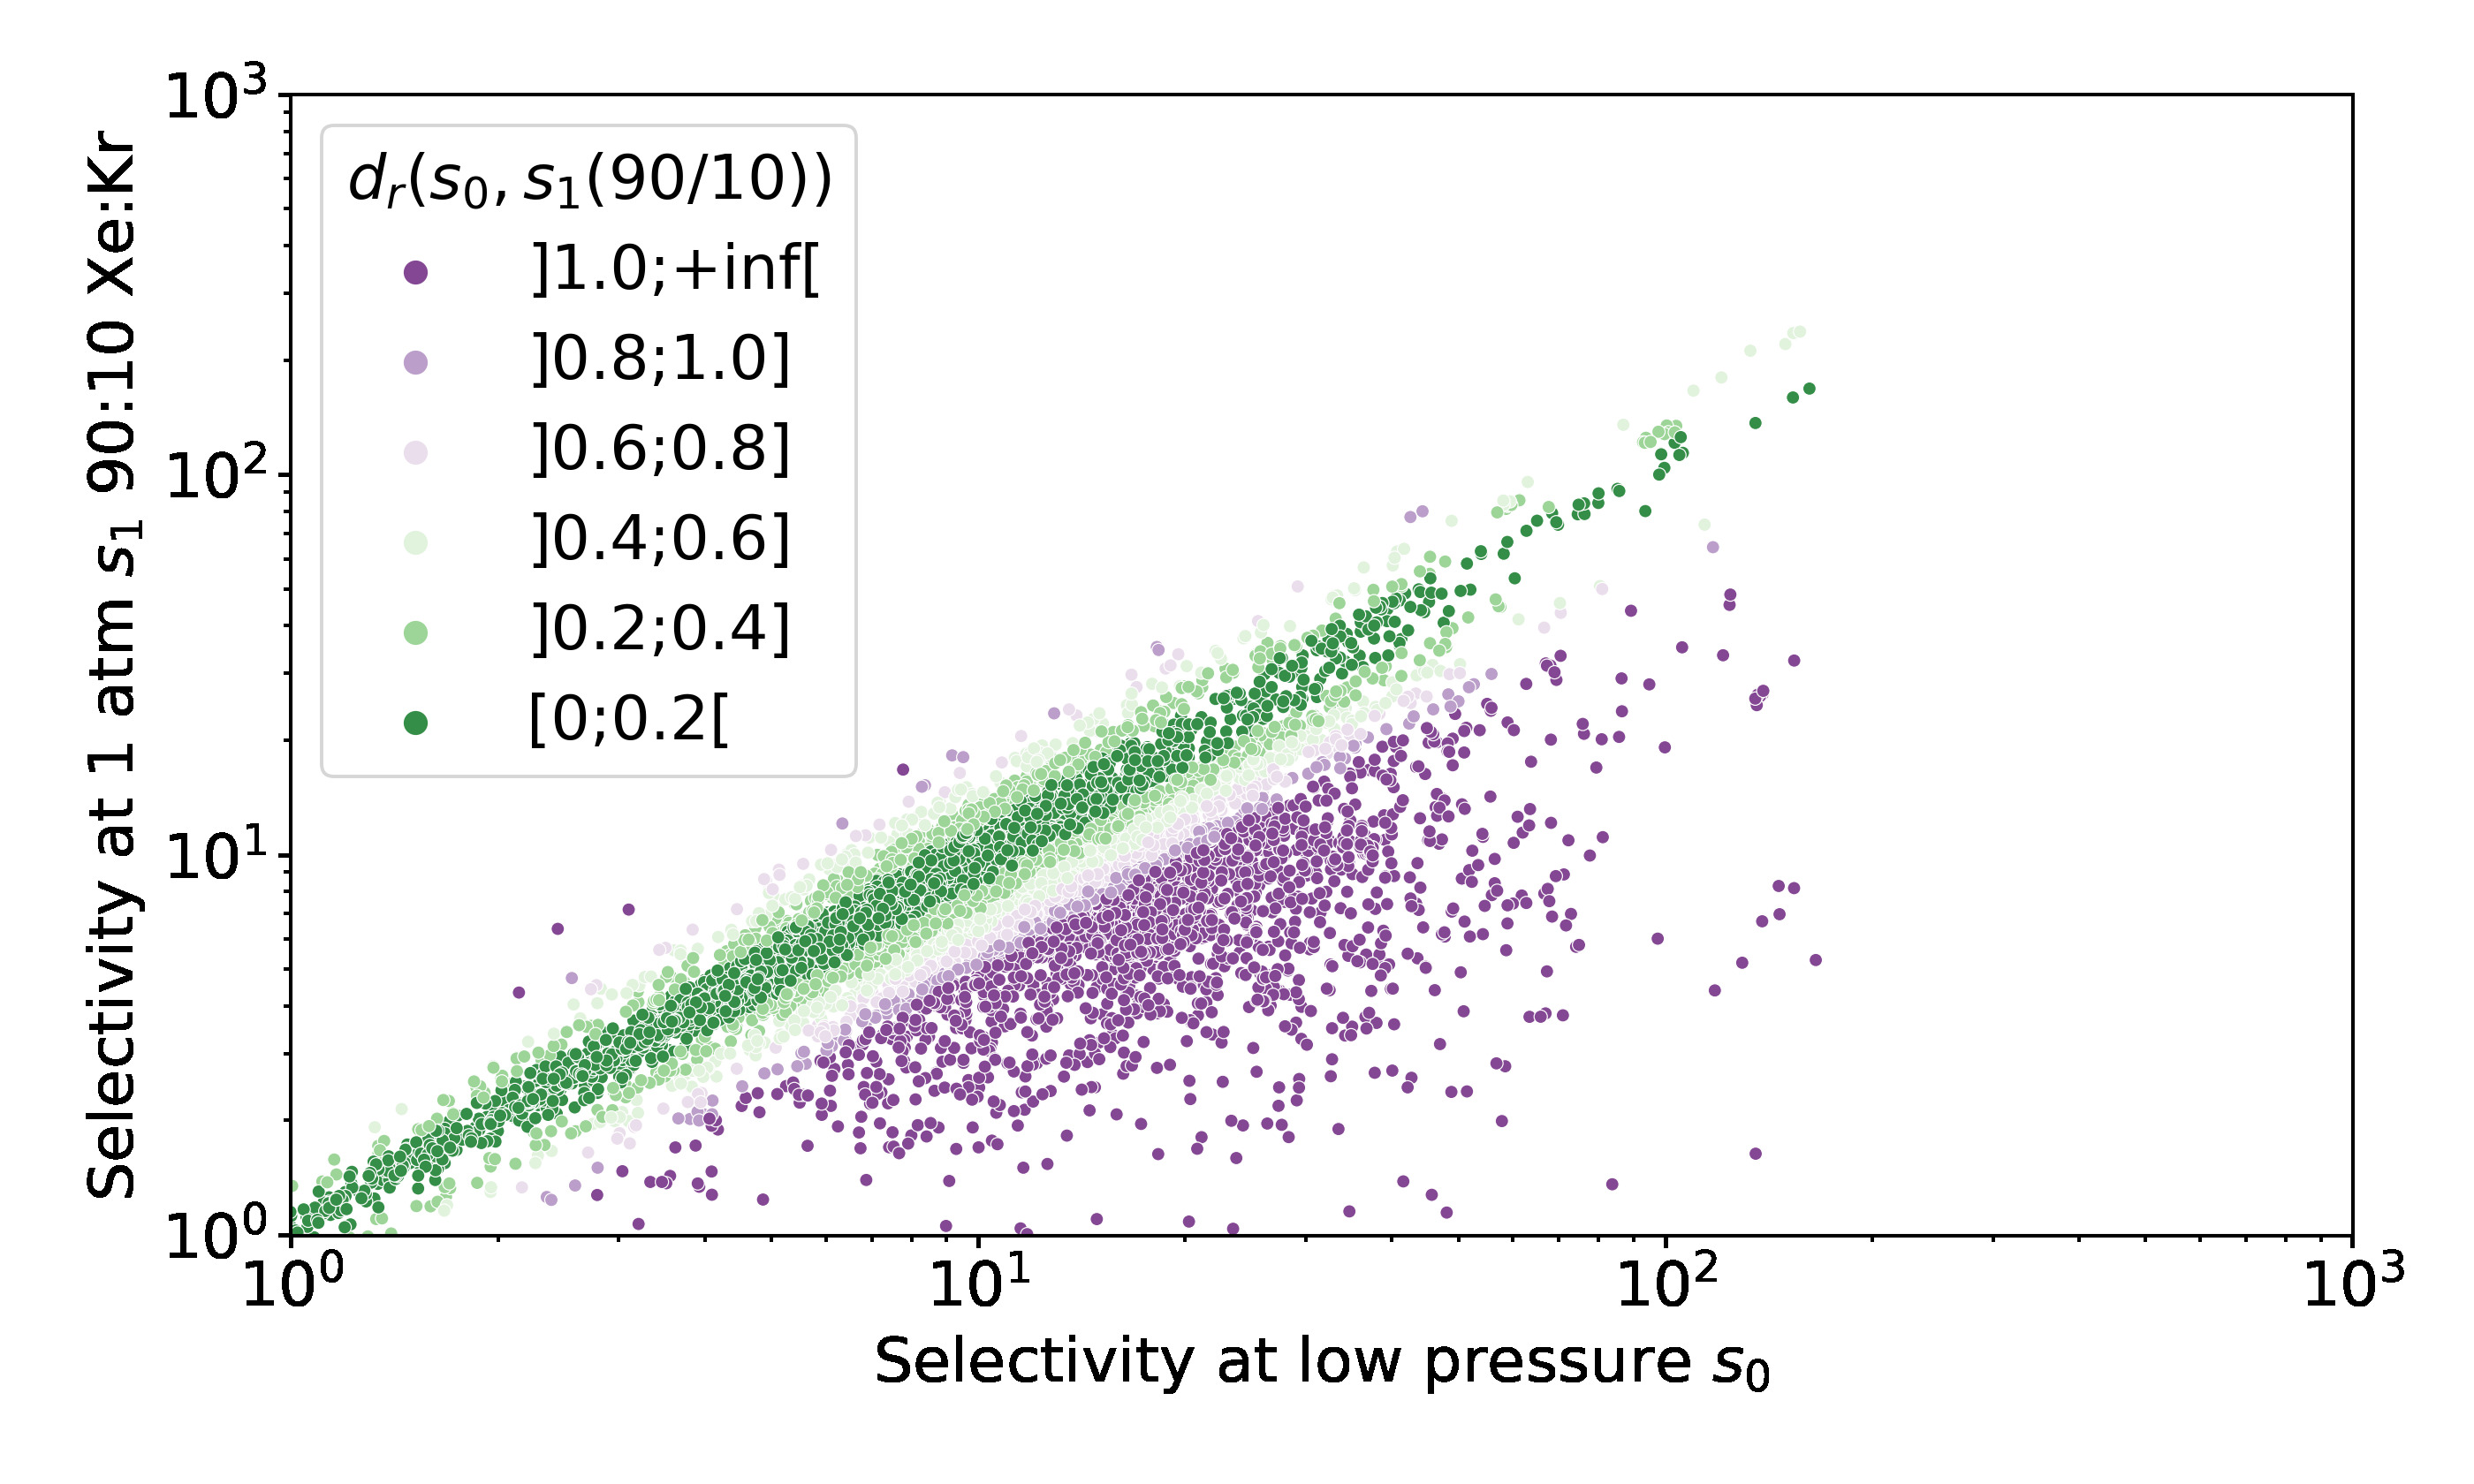
\includegraphics[width=0.6\linewidth]{figures/2-thermo/s_0_vs_s_9010_overview_log.jpg}
    \caption{Difference of selectivity between low pressure and at a \SI{1013}{\hecto\pascal} pressure for a 90:10 xenon krypton composition. The relative difference between the low-pressure selectivity and the ambient pressure is particularly high for the points labeled in purple.}
    \label{fgr:overview_9010}
\end{figure}
  
To evaluate quantitatively the thermodynamic effects at play in the competitive adsorption in different regimes, we can consider thermodynamic properties of the ``exchange equilibrium'' predefined in equation~\ref{eqn:exchange}. We plot in Figure~\ref{fgr:HSplot_0} the exchange entropy at low pressure (plotted as $T\Delta\e{exc}S\e{0}$) against the exchange enthalpy $\Delta\e{exc}H\e{0}$. In this scatterplot, the points are color-coded according to the selectivity $s\e{0}$ (with discrete categories for the sake of clarity), which is related to the enthalpy and entropy through Equation~\ref{eqn:entropy} --- meaning iso-selectivity lines are parallel straight lines in this scatterplot.
  
\begin{figure}[t]
\centering
  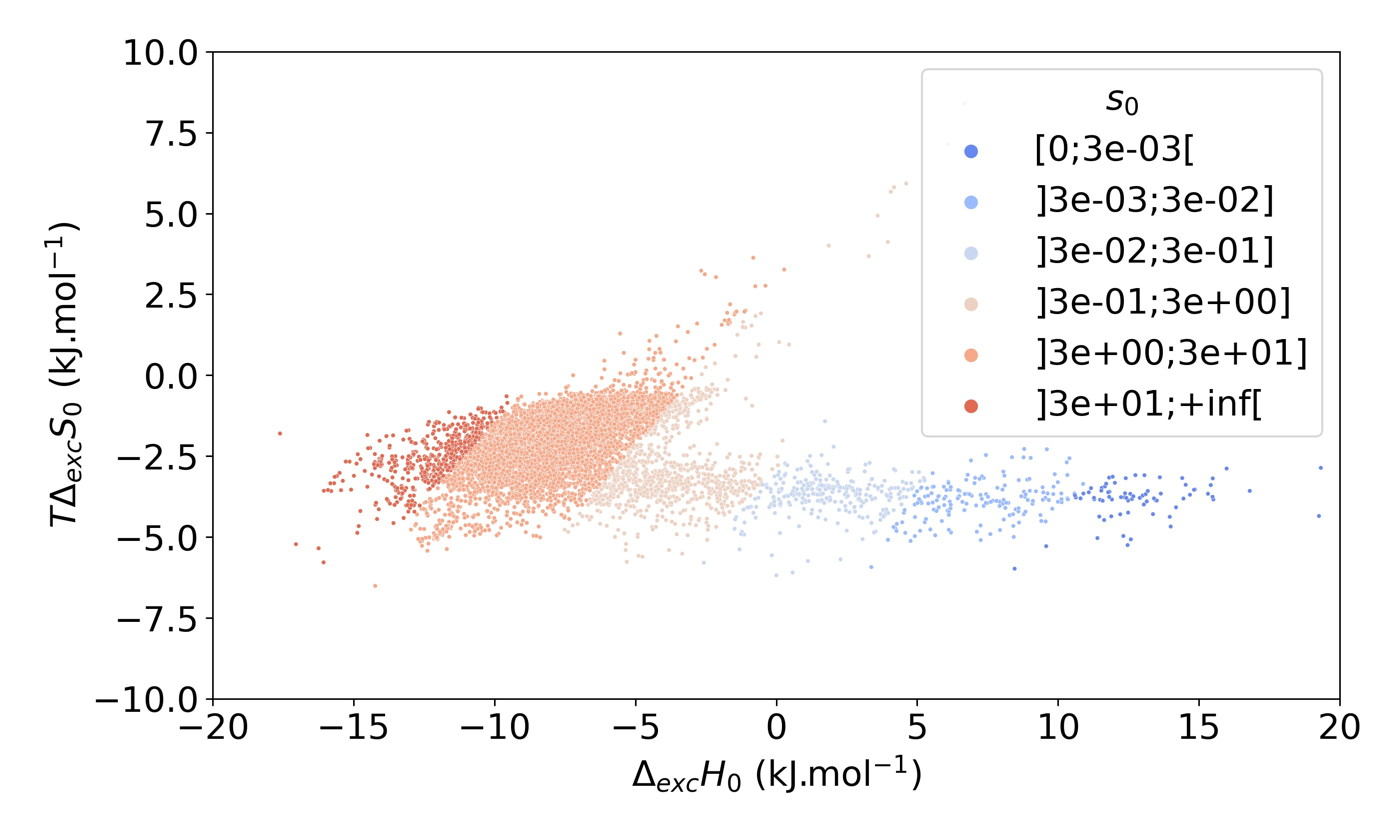
\includegraphics[width=0.6\linewidth]{figures/2-thermo/enthalpy_entropy_0_s_0.jpg}
  \caption{The energetic equivalent of exchange entropy $T\Delta\e{exc}S\e{0}$ and enthalpy $\Delta\e{exc}H\e{0}$ at low pressure labeled using the selectivity $s\e{0}$ at low pressure. The limits between labels follows an affine function of slope $1/T$ and of intercept $-R\ln(s\e{0}\ex{lim})$ where $s\e{0}\ex{lim}$ is the limit selectivity value (\emph{cf.} Equation~(\ref{eqn:exc_entropy})). In other words, the iso-selectivity lines are all parallel lines of equation $y=f(x)$ where $f$ is the affine function described previously.}
  \label{fgr:HSplot_0}
\end{figure}


\begin{figure}[t]
\centering
  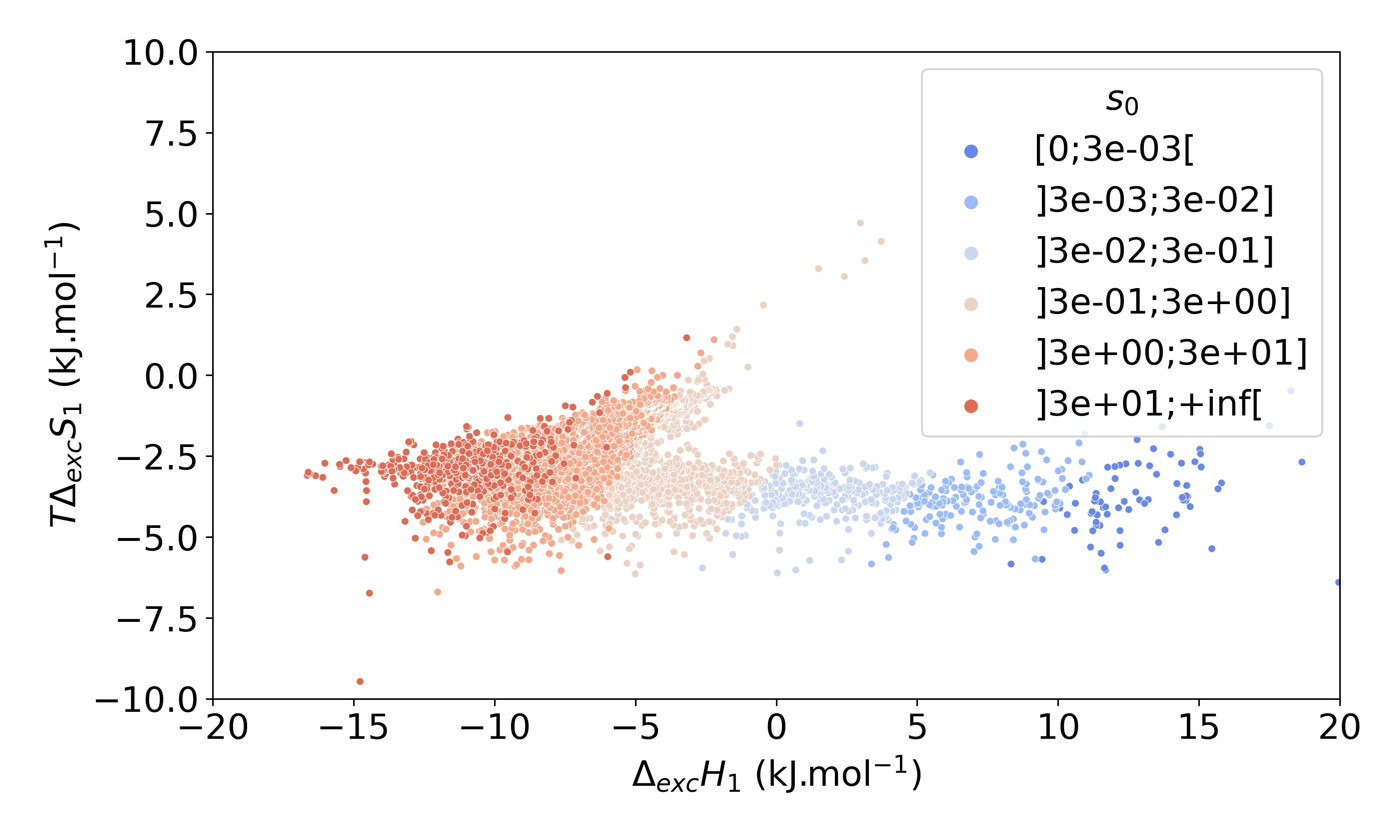
\includegraphics[width=0.6\linewidth]{figures/2-thermo/enthalpy_entropy_2080_s_0.jpg}
  \caption{The energetic equivalent of exchange entropy $T\Delta\e{exc}S\e{1}$ and enthalpy $\Delta\e{exc}H\e{1}$ at ambient pressure labeled using the selectivity $s\e{0}$ at low pressure. The points are layered so that the points with higher $s\e{0}$ are always above. To see a split version of this plot, please refer to the Figure~\ref{fgr:SI:dist1}.}
  \label{fgr:HSplot_1}
\end{figure}

\begin{figure*}[h]
  \centering
    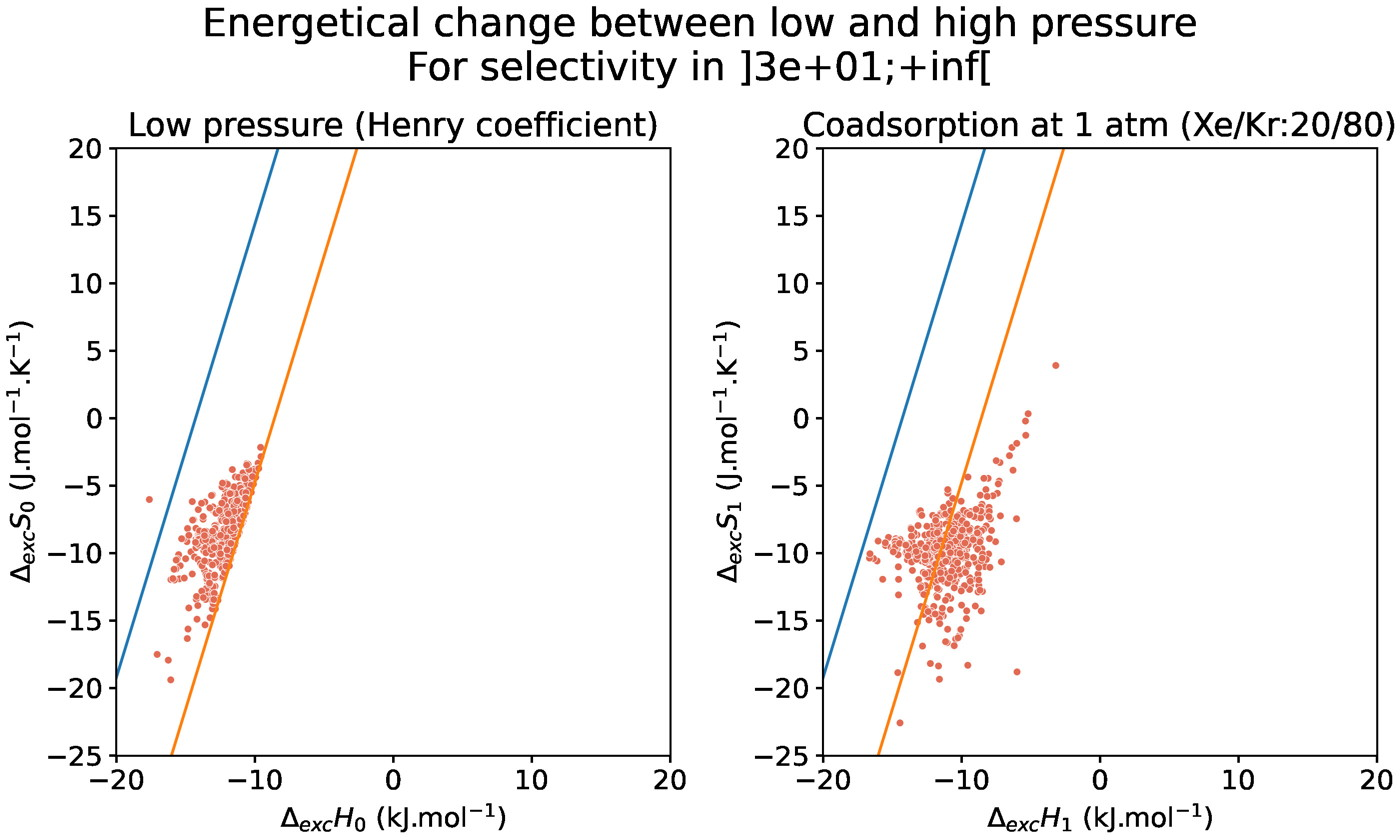
\includegraphics[width=0.45\textwidth]{figures/2-thermo/H_S_0.jpg}
    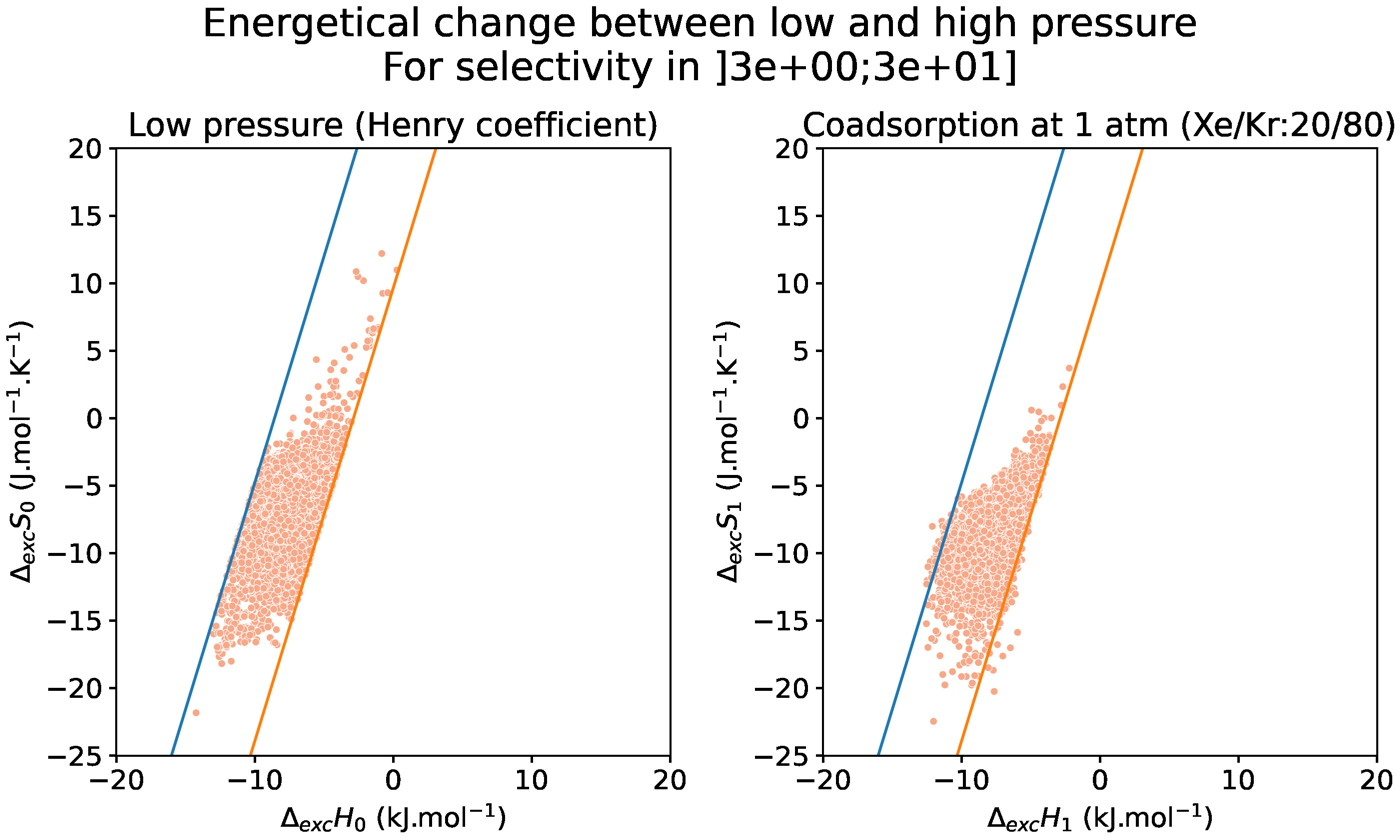
\includegraphics[width=0.45\textwidth]{figures/2-thermo/H_S_1.jpg}
    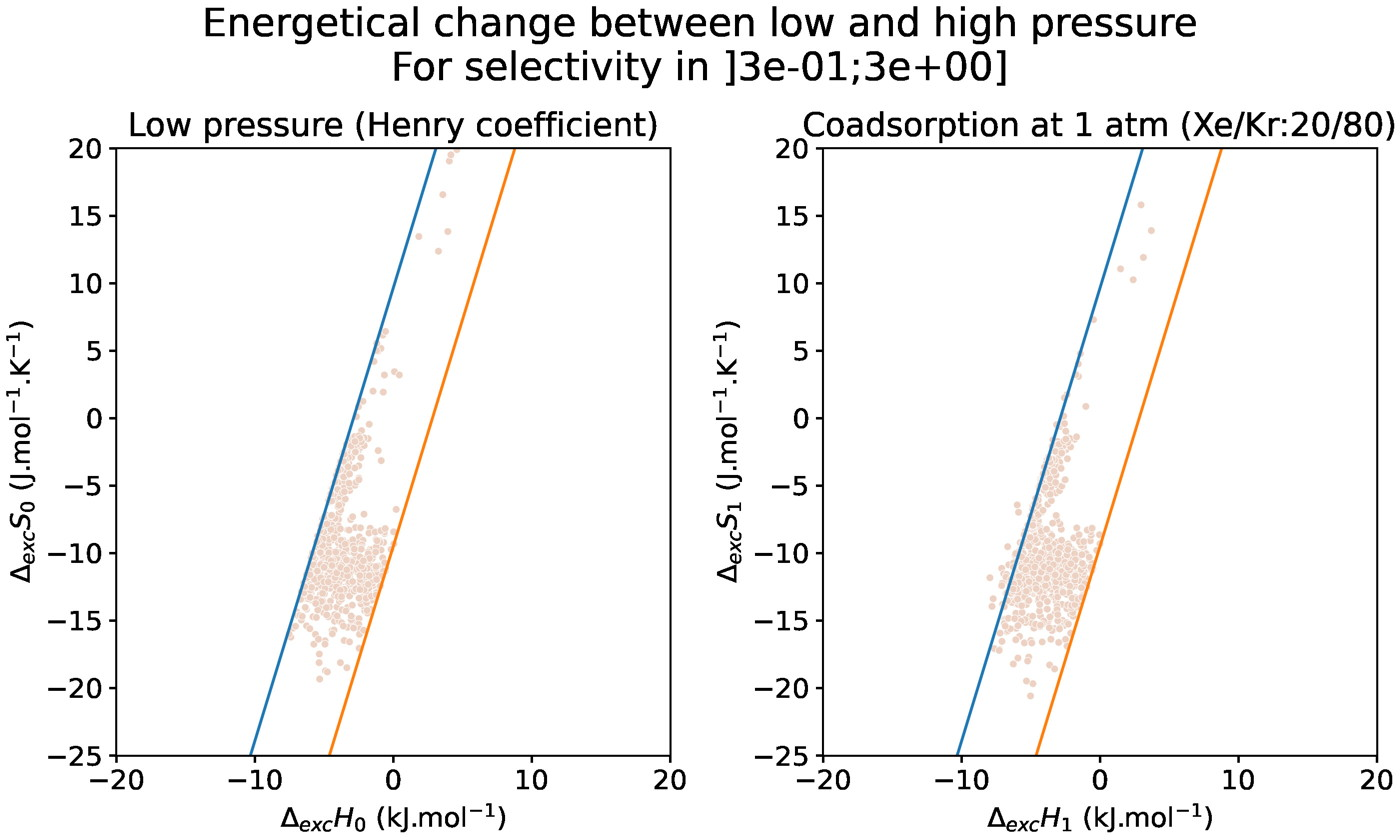
\includegraphics[width=0.45\textwidth]{figures/2-thermo/H_S_2.jpg}
    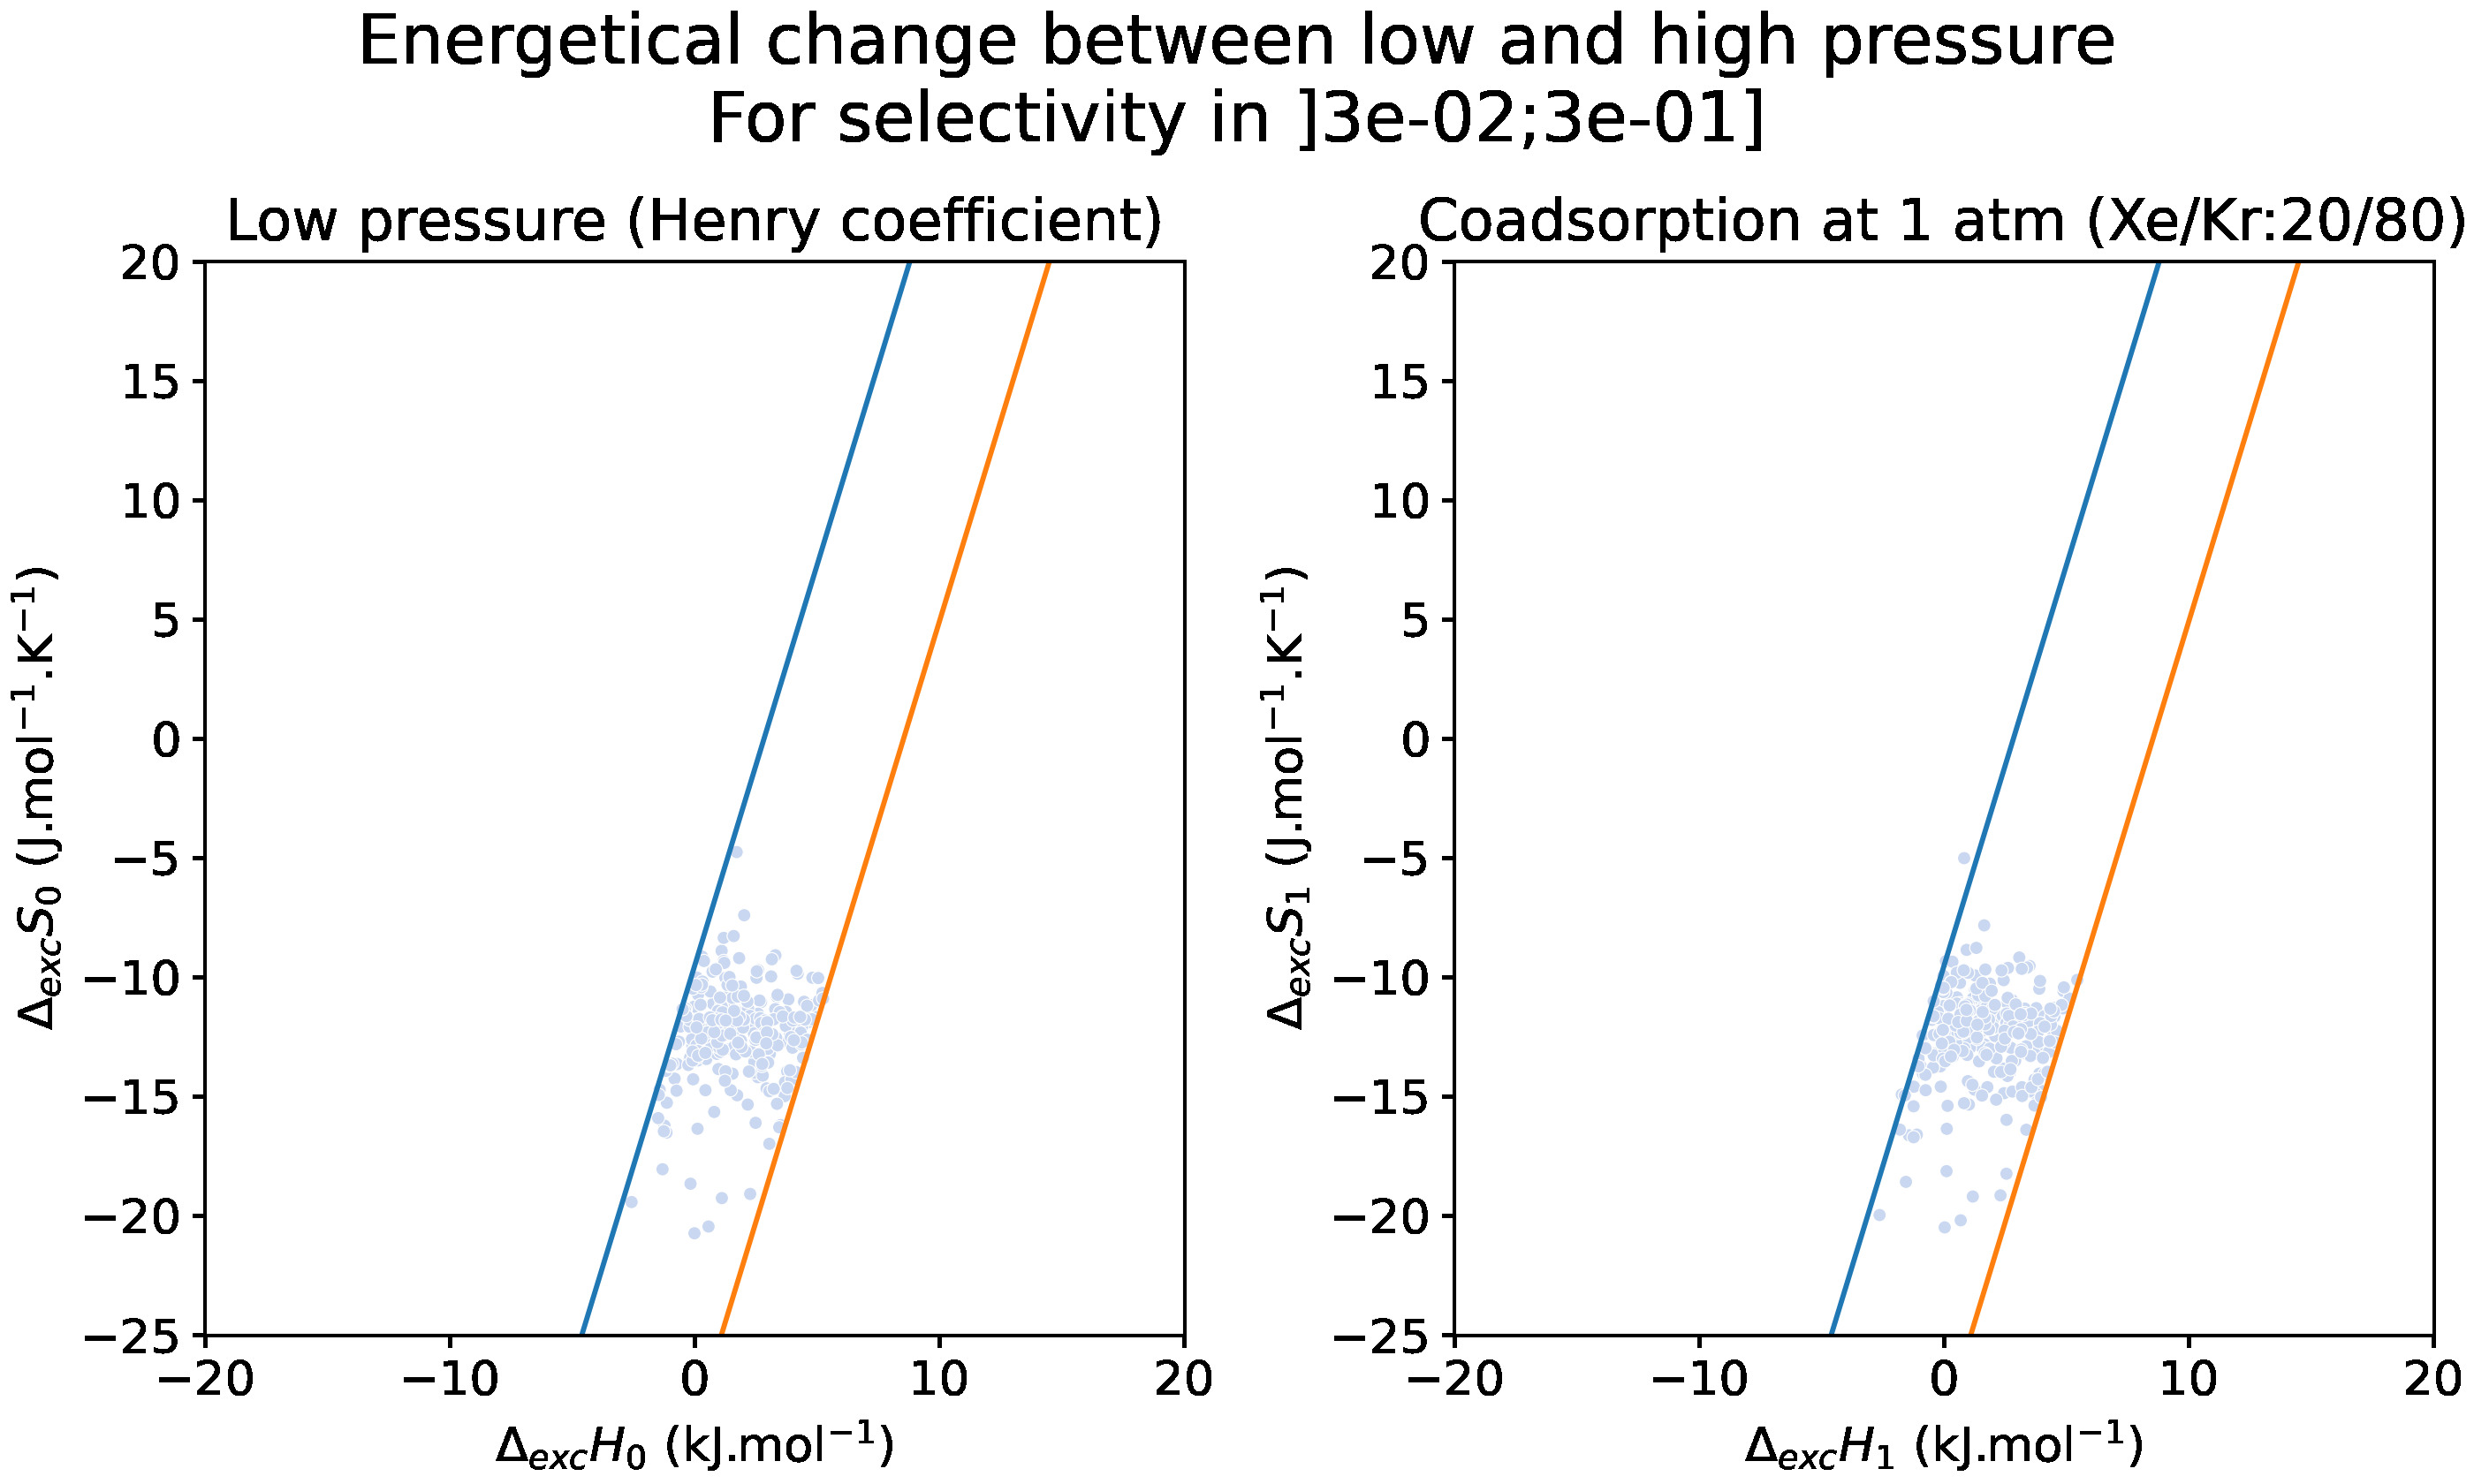
\includegraphics[width=0.45\textwidth]{figures/2-thermo/H_S_3.jpg}
    \caption{Split view of the Figure~\ref{fgr:HSplot_0} and \ref{fgr:HSplot_1}. The iso-selectivity lines for the limit considered are represented with blue and orange lines. We can clearly see the shift in exchange enthalpy for the structures with a selectivity higher than $30$.}
    \label{fgr:SI:dist1}
\end{figure*}


In the Figure~\ref{fgr:SI:dist0}, we display the distributions of the exchange enthalpy and entropy at low pressure. For the 630 most selective materials ($s\e{0} > 30$), the distribution of the exchange enthalpy $\Delta\e{exc}H\e{0}$ is centered on $-12.0$\,\si{\kilo\joule\per\mol} with a standard deviation of $1.3$\,\si{\kilo\joule\per\mol}, whereas the distribution of the exchange entropy (plotted as $T\Delta\e{exc}S\e{0}$) is centered on $-2.5$\,\si{\kilo\joule\per\mol} with a standard deviation of $0.7$\,\si{\kilo\joule\per\mol}. These figures, along with the overall distribution plotted in Figure~\ref{fgr:HSplot_0}, further confirms the moderate role of entropy in the low-pressure selectivity: it is equivalent in average to about {$20$\%} of the exchange enthalpy at low pressure.

Looking at the Figure~\ref{fgr:SI:dist1}, at ambient pressure, we can state the same conclusions on the limited influence of the entropy on the selectivity values. The distribution of the entropic term $T\Delta\e{exc}S\e{1}$ is now centered around $-3$~\si{\kilo\joule\per\mole}, which is also quite small in comparison of the values of $\Delta\e{exc}H\e{1}$. For the most selective materials, the entropic term represents about {$19$\%} of the exchange enthalpy at ambient pressure.

\begin{figure*}[h]
  \centering
    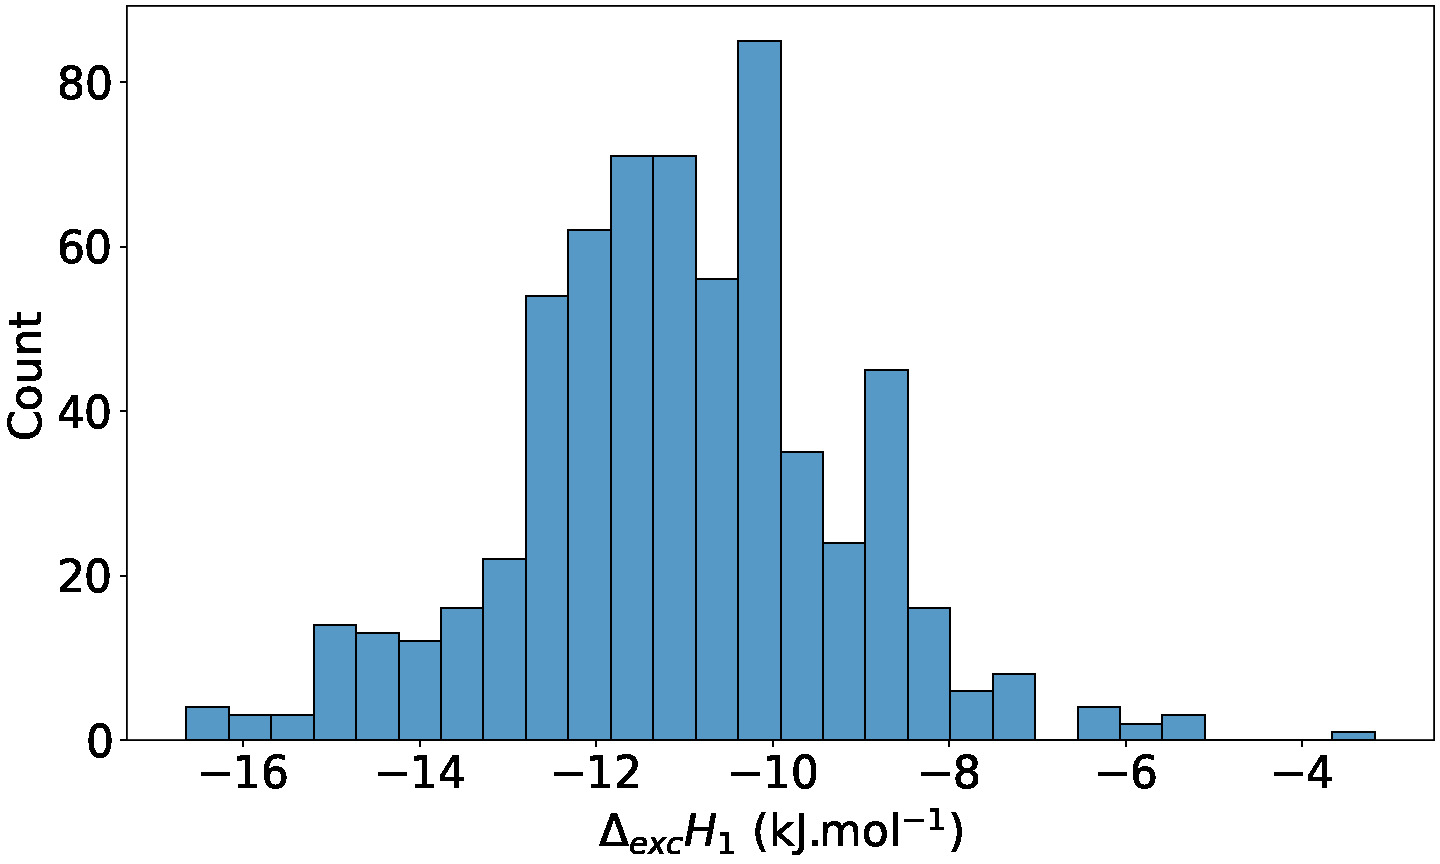
\includegraphics[width=0.45\textwidth]{figures/2-thermo/Delta_H_2080.jpg}
    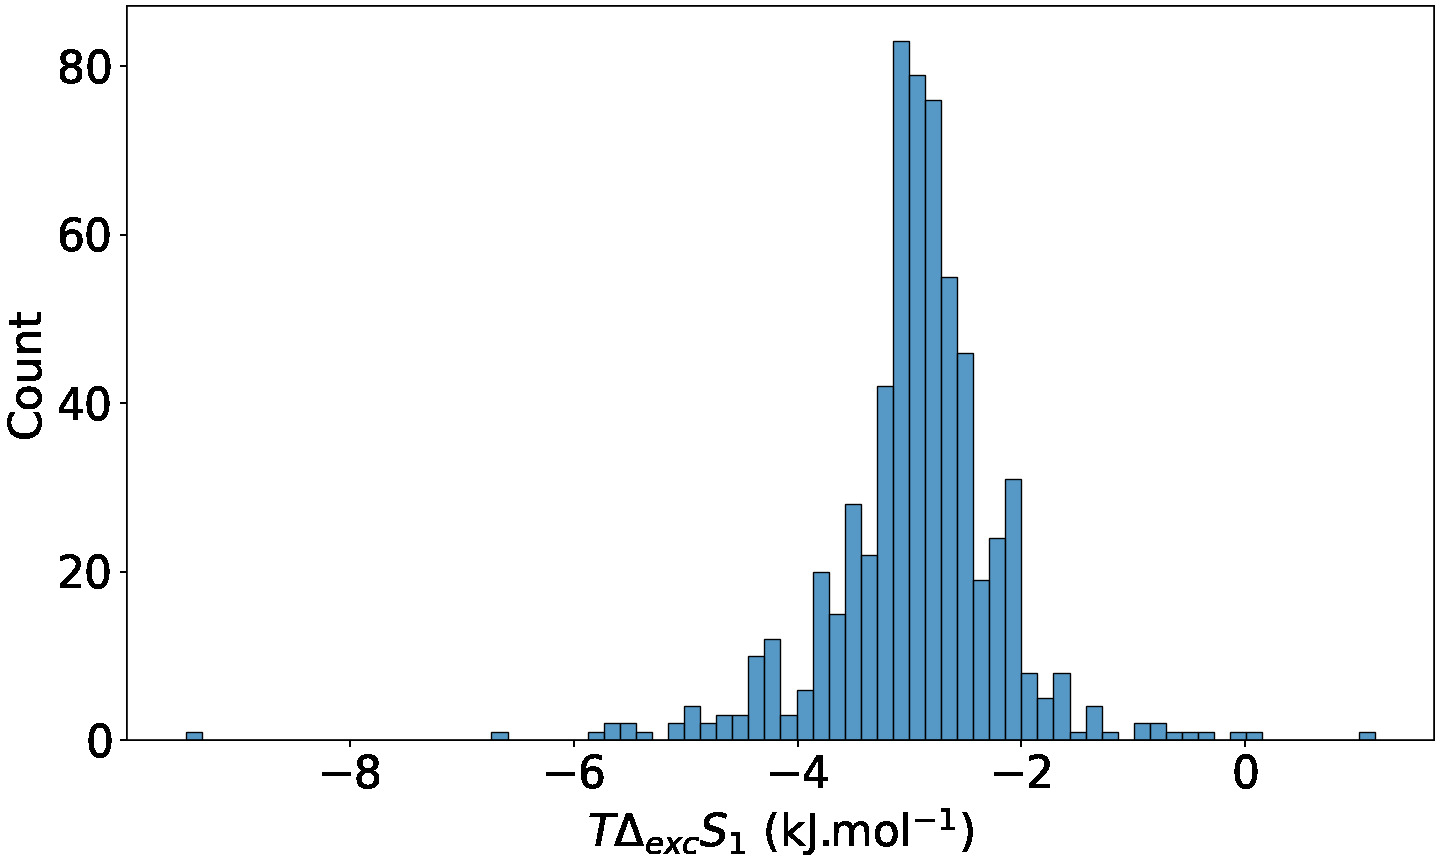
\includegraphics[width=0.45\textwidth]{figures/2-thermo/T_Delta_S_2080.jpg}
    \caption{Distribution of the enthalpy $\Delta\e{exc}H\e{1}$ and entropic term $T\Delta\e{exc}S\e{1}$ of exchange at ambient pressure on the 630 most selective structures.}
    \label{fgr:SI:dist1}
\end{figure*}

Figure~\ref{fgr:HSplot_1} represents a scatterplot of the exchange entropy at $P = 1$\,atm $\Delta\e{exc}S\e{1}$ against the exchange enthalpy at ambient pressure $\Delta\e{exc}H\e{1}$. To compare it to the Fig.~\ref{fgr:HSplot_0}, the points are color-coded according to the low-pressure selectivity $s\e{0}$. Compared to the iso-selectivity $s\e{1}$ straight parallel lines (\emph{c.f.}~Figure~\ref{fgr:SI:dist1}), we can see that many materials with high $s\e{0}$ have lower $s\e{1}$ --- seen as a migration of points to the right of the plot, compared to Fig.~\ref{fgr:HSplot_0}. This shift is therefore mainly due to a higher (less favorable) exchange enthalpy, hinting at an important role of enthalpy to determine higher pressure selectivity.

To quantify this change, we consider the distributions of the exchange enthalpy $\Delta\e{exc}H\e{1}$ and the energetic equivalent of the exchange entropy $T\Delta\e{exc}S\e{1}$ at ambient pressure (Figure~\ref{fgr:SI:dist1}). The enthalpy $\Delta\e{exc}H\e{1}$ is now centered on $-11.1$\,\si{\kilo\joule\per\mol} with a standard deviation of $1.9$\,\si{\kilo\joule\per\mol}. Compared to the zero-pressure values, the enthalpy distribution is more dispersed, showing that there are important changes in individual values, and is higher in average --- majority of materials have lower ambient pressure selectivity due to enthalpic effects. This can be explained by the very general increase of adsorption enthalpy upon loading in the gas phase, which is linked to the presence of more adsorbed molecules. In fact, the correlations (Figure \ref{fgr:histo_K}) suggest that highly selective materials have high affinity in xenon; therefore they feature significant uptake at \SI{1}{\atm} and the large Xe loading means the most favorable adsorption sites can be saturated, and further adsorption involves weaker host--guest interactions and therefore increases the average adsorption enthalpy at non-zero loading.

The entropic term $T\Delta\e{exc}S\e{1}$ is now centered on $-2.9$\,\si{\kilo\joule\per\mol}, with a standard deviation of $0.8$\,\si{\kilo\joule\per\mol} (almost unchanged from low-pressure). The entropy is on average lower, which means an overall less favorable separation due to entropic effects: this evolution of the entropic term hints at the potential of a reorganization of the adsorbed molecules inside each material. The difference in distribution of enthalpy has, overall, more impact on the high-pressure selectivity than that of entropy. This suggests that the overall contribution of enthalpy remains more decisive than the role of entropy in the selectivity change, even at ambient pressure. This is an interesting conclusion for screening studies, because evaluation of adsorption enthalpy can be computationally faster than that of the adsorption free energy (or entropy).

\begin{figure*}[t]
  \centering
    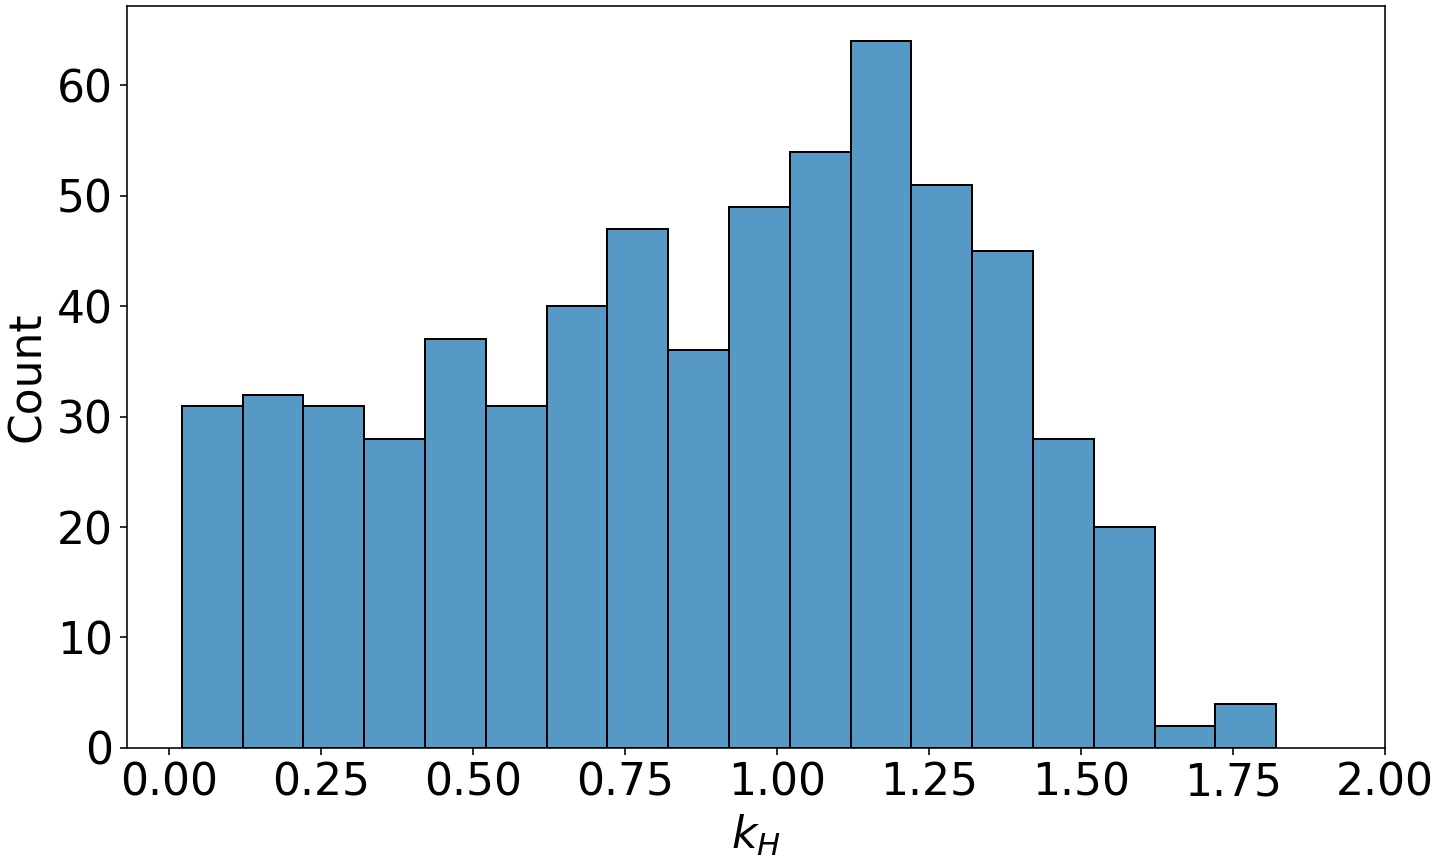
\includegraphics[width=0.37\textwidth]{figures/2-thermo/k_H.jpg}
    \hspace{8mm}
    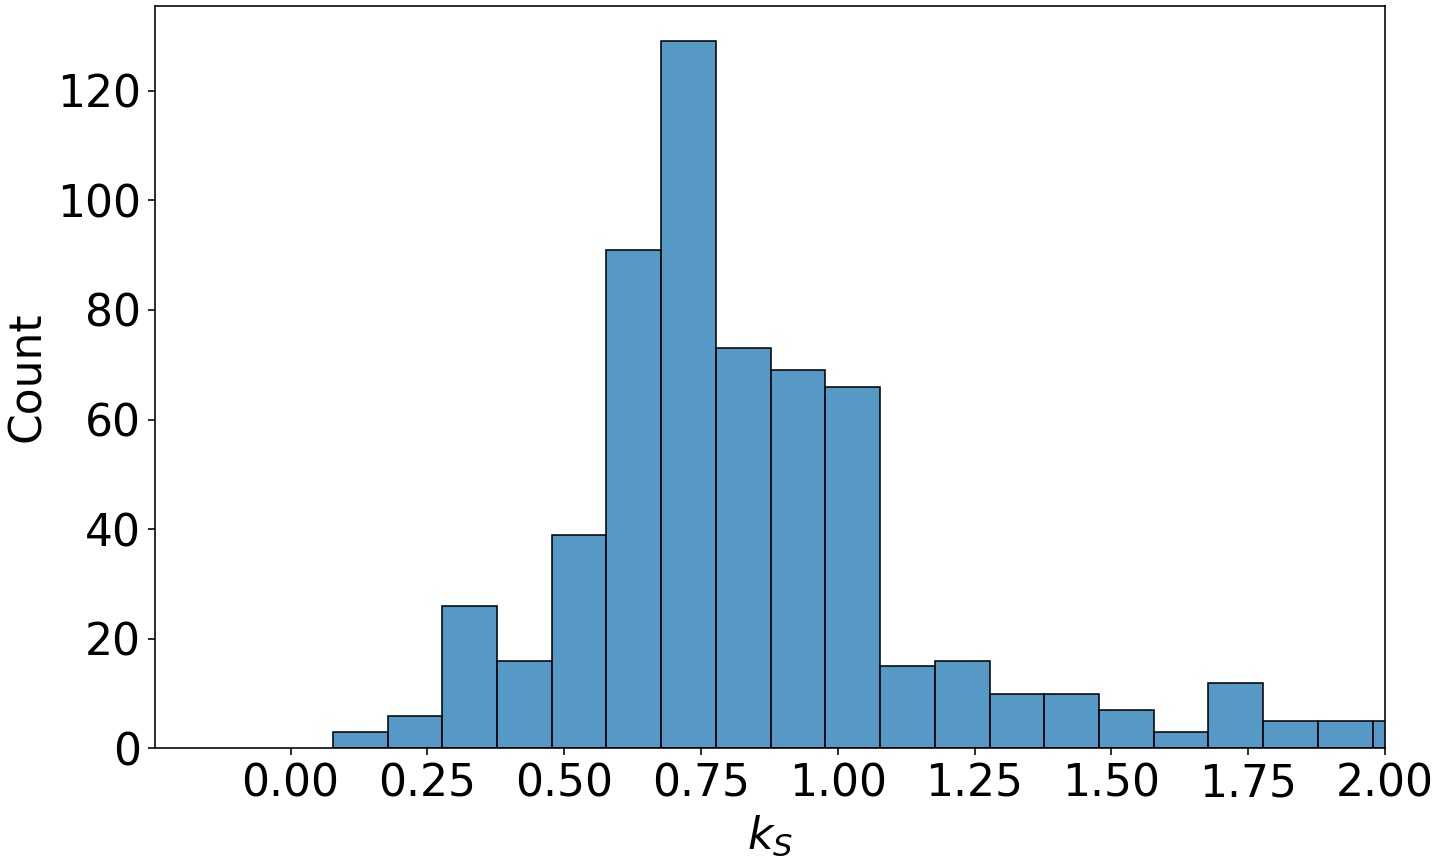
\includegraphics[width=0.37\textwidth]{figures/2-thermo/k_S.jpg}
    \caption{Distribution of the enthalpic $k\e{H}$ and entropic $k\e{S}$ contributions to the change of selectivity from low to ambient pressure for the 630 materials with $s\e{0}>30$. $k\e{H}$ has a rather uniform distribution, whereas $k\e{S}$ has a bell-like distribution. }
    \label{fgr:distk}
\end{figure*}

\begin{figure}[t]
\centering
  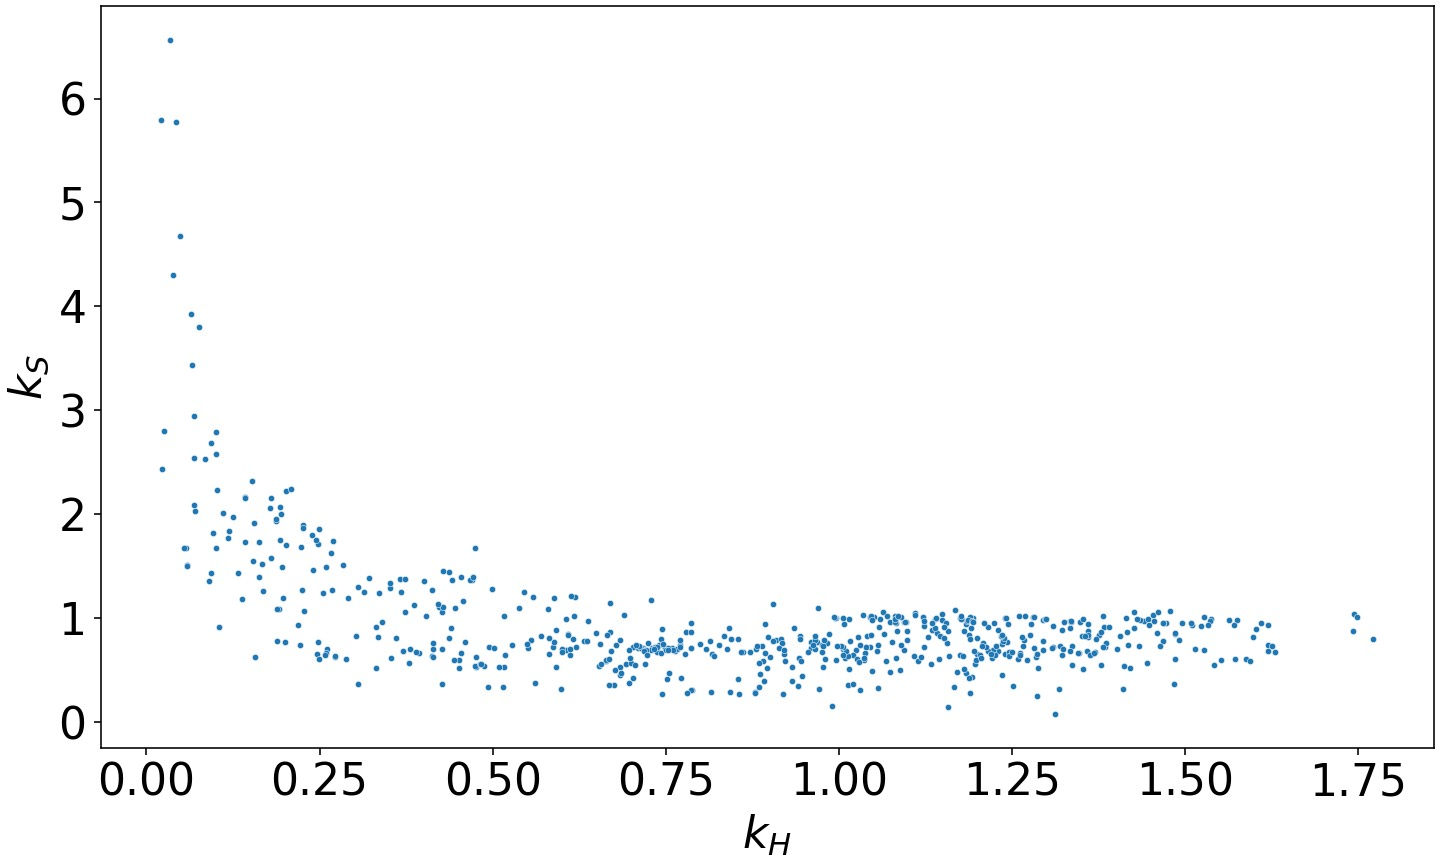
\includegraphics[width=0.45\textwidth]{figures/2-thermo/k_S_vs_k_H.jpg}
  \caption{Scatterplot of the enthalpic contribution $k\e{H}$ and entropic contribution $k\e{S}$ for the 630 materials with $s\e{0}>30$. The entropic compensation occurs when the enthalpic contribution is around $0.1$, else its value is around 1 and has little effect on the selectivity change.}
  \label{fgr:scatterk}
\end{figure}
  
To further investigate the thermodynamics of the selectivity change, we quantify in this section the contributions of enthalpy and entropy. The ratio ${s\e{1}}/{s\e{0}}$ is equal to the product $k\e{H} \times k\e{S}$ where $k\e{H}$ and $k\e{S}$ are the enthalpic and entropic contributions to the selectivity change defined as:
\begin{equation}
\label{eqn:effects}
    \begin{split}
      k\e{H} & = \exp\left(-\dfrac{\Delta\e{exc}H\e{1}-\Delta\e{exc}H\e{0}}{RT}\right) \\ k\e{S} & = \exp\left(\dfrac{\Delta\e{exc}S\e{1}-\Delta\e{exc}S\e{0}}{R}\right)
    \end{split}
\end{equation}
As we can see in Figure~\ref{fgr:distk}, the entropic contribution $k\e{S}$ has a bell-like distribution, with a mean of $0.9$ and a standard deviation of $0.6$. This confirms that $k\e{S}$ is close to $1$, and has therefore only a marginal effect on the selectivity change. On the other hand, the enthalpic contribution $k\e{H}$ has a more uniform distribution ranging from $0.1$ to $1.5$, which means that enthalpy has a crucial role in the selectivity change we observe. There are a significant number of materials with a $k\e{H}$ close to zero, they correspond to the same materials highlighted in Section~\ref{section:pressure}.

Furthermore, the scatterplot of $k\e{H}$ and $k\e{S}$ (shown in Figure~\ref{fgr:scatterk}) confirms a rather moderate effect of entropy. For most of the materials with $0.25 \le k\e{H} \le 1.75$, we see that $k\e{S}$ is close to 1. The most significant entropic contributions are found for materials where $k\e{H}$ is close to zero (typically below 0.25). If we look in more detail at the 29 materials with $k\e{S}>2$, the entropic contribution $k\e{S}$ moderately compensate the enthalpic contribution as the average ratio $s\e{1}/s\e{0}$ is around $0.25$. In such cases, the entropy is non-negligible and it can partially compensate the enthalpic contribution to the selectivity change, but the general trend is still given by enthalpy, since the overall selectivity is decreasing as a result.
  
\subsection{Detailed investigation}
\label{sec:archetypes}

\begin{table}[hb]
  \small
    \caption{Enthalpic ($k\e{H}$) and entropic ($k\e{S}$) contributions to the selectivity change ($s\e{1}/s\e{0}$) between low and ambient pressures for some archetypal structures selected for their high $s\e{0}$ selectivity at infinite dilution. Every structure is identified using a CSD Refcode and a reference the first article that mentions it. The pore size is also characterized using the global cavity diameter (GCD) and the pore limiting diameter (PLD) values in \si{\angstrom}.}
    \label{tbl:effect}
    \renewcommand{\arraystretch}{1.1}
    \begin{tabular*}{0.8\textwidth}{@{\extracolsep{\fill}}|lr|rrrrr|rr|}
      \hline
        CSD Refcode & Ref. & $s\e{0}$ &  $s\e{1}$  &  $s\e{1}/s\e{0}$ &  $k\e{H}$ &  $k\e{S}$ & GCD & PLD\\
      \hline
      VOKJIQ & \cite{VOKJIQ} &           $157.17$ &  $242.73$ &  $1.54$ &  $1.46$ &  $1.06$  &  $5.2$  &  $3.2$  \\
      KAXQIL & \cite{KAXQIL} &           $103.78$ &  $132.57$ &  $1.28$ &  $1.32$ &  $0.96$  &  $5.2$  &  $4.1$  \\
      JUFBIX & \cite{JUFBIX} &           $106.11$ &  $114.83$ &  $1.08$ &  $1.08$ &  $1.00$  &  $5.3$  &  $3.0$  \\
      FALQOA & \cite{FALQOA} &           $162.20$ &  $171.10$ &  $1.05$ &  $1.09$ &  $0.96$  &  $5.1$  &  $3.5$  \\
      GOMREG & \cite{GOMREG_GOMRAC} &    $114.14$ &  $ 73.83$ &  $0.65$ &  $1.01$ &  $0.64$  &  $5.8$  &  $4.0$  \\
      JAVTAC & \cite{JAVTAC} &           $117.38$ &  $ 66.93$ &  $0.57$ &  $0.77$ &  $0.74$  &  $5.5$  &  $4.3$  \\
      GOMRAC & \cite{GOMREG_GOMRAC} &    $124.11$ &  $ 47.34$ &  $0.38$ &  $0.58$ &  $0.66$  &  $5.7$  &  $3.7$  \\
      MISQIQ & \cite{MISQIQ} &           $138.94$ &  $ 37.32$ &  $0.27$ &  $0.51$ &  $0.53$  &  $4.6$  &  $4.4$  \\
    BAEDTA01 & \cite{BAEDTA01} &         $154.10$ &  $ 37.74$ &  $0.24$ &  $0.12$ &  $1.97$  &  $5.7$  &  $4.6$  \\
      VIWMOF & \cite{VIWMOF} &           $ 81.13$ &  $ 13.24$ &  $0.16$ &  $0.04$ &  $4.30$  & $10.2$  &  $5.3$  \\
      LUDLAZ & \cite{LUDLAZ} &           $165.68$ &  $ 16.42$ &  $0.10$ &  $0.16$ &  $0.63$  &  $6.7$  &  $4.2$  \\
      WOJJOV & \cite{WOJJOV} &           $146.32$ &  $ 13.94$ &  $0.10$ &  $0.06$ &  $1.68$  &  $8.2$  &  $6.8$  \\
      VAPBIZ & \cite{VAPBIZ} &           $146.73$ &  $ 12.76$ &  $0.09$ &  $0.06$ &  $1.50$  &  $6.3$  &  $3.7$  \\
      \hline 
  \end{tabular*}
\end{table}

In this section, we go over some of the most selective materials, as identified at low pressure and listed in Table~\ref{tbl:effect}, and we provide a detailed investigation of the thermodynamic effects behind their behavior. We can split them into three main categories: materials with a slight increase in selectivity or little change in selectivity ($s\e{0}/s\e{1} > 0.8$), materials with a slight decrease in selectivity ($0.5 \le s\e{0}/s\e{1} \le 0.8$) and materials with a significant decrease in selectivity ($s\e{0}/s\e{1} < 0.5$). In this section, we investigate the origins of these different behaviors: all materials are referenced by their CSD refcode.

  
\begin{table*}[hb]
\fontsize{8.5}{10.5}\selectfont
  \caption{\ Thermodynamic quantities associated for a few archetypal structures. Henry's constant $K\ex{Xe}$, $K\ex{Kr}$ are in \si{\milli\mol\per\gram\per\pascal}, loadings $q\ex{Xe}\e{1}$ and $q\ex{Kr}\e{1}$ are in \si{\milli\mol\per\gram}, enthalpies $\Delta\e{ads}H\ex{Xe}\e{0}$, $\Delta\e{ads}H\ex{Xe}\e{0}$, $\Delta\e{ads}H\ex{Xe}\e{1}$ and $\Delta\e{ads}H\ex{Xe}\e{1}$ are in \si{\kilo\joule\per\mol} }\label{tbl:thermo}
  \label{tbl:example}
    \renewcommand{\arraystretch}{1.5}
    \begin{tabular}{|lr|rrrrr|rrrrr|}
    \hline
          CSD Refcode & Ref. &  $s\e{0}$ &  $K\ex{Xe}$ &  $K\ex{Kr}$ &  $\Delta\e{ads}H\ex{Xe}\e{0}$ &  $\Delta\e{ads}H\ex{Kr}\e{0}$  &  $s\e{1}$ &  $q\ex{Xe}\e{1}$ &  $q\ex{Kr}\e{1}$ &  $\Delta\e{ads}H\ex{Xe}\e{1}$ &  $\Delta\e{ads}H\ex{Xe}\e{1}$ \\
    \hline
        VOKJIQ & \cite{VOKJIQ}        &  $157$  &  $7.92\,10^{-1}$  &  $5.04\,10^{-3}$  &  $-53.9$  &  $-38.2$  &  $243$  &  $2.57$  &  $0.04$  &  $-61.1$  &  $-44.5$  \\
        KAXQIL & \cite{KAXQIL}        &  $104$  &  $3.01\,10^{-2}$  &  $2.90\,10^{-4}$  &  $-44.6$  &  $-30.5$  &  $133$  &  $1.41$  &  $0.04$  &  $-41.5$  &  $-26.8$  \\
        JUFBIX & \cite{JUFBIX}        &  $106$  &  $1.59\,10^{-2}$  &  $1.50\,10^{-4}$  &  $-45.6$  &  $-31.4$  &  $115$  &  $0.80$  &  $0.03$  &  $-45.7$  &  $-31.3$  \\
        FALQOA & \cite{FALQOA}        &  $162$  &  $2.23\,10^{-2}$  &  $1.38\,10^{-4}$  &  $-47.3$  &  $-32.0$  &  $171$  &  $0.68$  &  $0.02$  &  $-48.6$  &  $-33.1$  \\
        GOMREG & \cite{GOMREG_GOMRAC} &  $114$  &  $9.16\,10^{-2}$  &  $8.03\,10^{-4}$  &  $-44.7$  &  $-31.1$  &  $ 74$  &  $2.59$  &  $0.14$  &  $-47.5$  &  $-33.8$  \\
        JAVTAC & \cite{JAVTAC}        &  $117$  &  $1.24\,10^{-1}$  &  $1.06\,10^{-3}$  &  $-47.7$  &  $-33.5$  &  $ 67$  &  $1.50$  &  $0.09$  &  $-48.5$  &  $-34.9$  \\
        GOMRAC & \cite{GOMREG_GOMRAC} &  $124$  &  $1.17\,10^{-1}$  &  $9.45\,10^{-4}$  &  $-45.6$  &  $-31.8$  &  $ 47$  &  $2.51$  &  $0.21$  &  $-47.3$  &  $-34.8$  \\
        MISQIQ & \cite{MISQIQ}        &  $139$  &  $6.87\,10^{-1}$  &  $4.94\,10^{-3}$  &  $-51.9$  &  $-37.4$  &  $ 37$  &  $2.30$  &  $0.25$  &  $-45.6$  &  $-32.8$  \\
      BAEDTA01 & \cite{BAEDTA01}      &  $154$  &  $1.39\,10^{-2}$  &  $9.04\,10^{-5}$  &  $-47.7$  &  $-31.7$  &  $ 38$  &  $1.05$  &  $  11$  &  $-34.0$  &  $-23.1$  \\
        VIWMOF & \cite{VIWMOF}        &  $ 81$  &  $7.87\,10^{-3}$  &  $9.70\,10^{-5}$  &  $-46.3$  &  $-30.1$  &  $ 13$  &  $2.99$  &  $0.90$  &  $-26.0$  &  $-17.8$  \\
        LUDLAZ & \cite{LUDLAZ}        &  $166$  &  $9.04\,10^{-2}$  &  $5.46\,10^{-4}$  &  $-45.4$  &  $-30.9$  &  $ 16$  &  $1.59$  &  $0.39$  &  $-38.3$  &  $-28.3$  \\
        WOJJOV & \cite{WOJJOV}        &  $146$  &  $4.19\,10^{-2}$  &  $2.86\,10^{-4}$  &  $-46.4$  &  $-30.7$  &  $ 14$  &  $2.82$  &  $0.81$  &  $-33.0$  &  $-24.4$  \\
        VAPBIZ & \cite{VAPBIZ}        &  $147$  &  $3.54\,10^{-2}$  &  $2.41\,10^{-4}$  &  $-46.4$  &  $-30.5$  &  $ 13$  &  $2.50$  &  $0.78$  &  $-34.1$  &  $-25.3$  \\
    \hline
    \end{tabular}
\end{table*}

Before introducing the different archetypal structures that undergo different changes in selectivity, let us bring in some notions on adsorption isotherms. The isotherms are representation of the adsorbed quantity as a function of the pressure for different components at a given temperature. Here, we will only tackle the case of pure-component isotherms at \SI{298}{\kelvin}. Different models have been developed to interpret these plots,\cite{Al_Ghouti_2020} but here we will only use the Langmuir model as it is the most prominent equation to explain adsorption equilibria. The Langmuir model is a local model of adsorption based on the filling of a monolayer by non-interacting adsorbates. Depending on the distribution and shape of the pores, these isotherms can be either modeled by a 1-site Langmuir or a 2-site Langmuir model. At given temperature, some mono-site materials' isotherm can be described by the following equation:
\begin{equation}\label{eq:langmuir_1}
    q(P) = N\e{max}\dfrac{KP}{1+KP}
\end{equation}
where $q$ is the adsorbed quantity of a mono-component gas, $K$ is the adsorption equilibrium constant and $P$ is the pressure. When the material has 2 sites, the isotherm can be described by the following equation:
\begin{equation}\label{eq:langmuir_2}
    q(P) = N\e{max}\left((1-\alpha\e{2})\dfrac{K\e{1}P}{1+K\e{1}P}+\alpha\e{2}\dfrac{K\e{2}P}{1+K\e{2}P}\right)
\end{equation}
where $q$ is the loading of a given mono-component gas, $K_1$ and $K_2$ are the adsorption equilibrium constants in the respective sites, $\alpha\e{2}$ is the proportion of secondary sites, and $P$ is the pressure.
  
We first study a few examples of the category of materials where ambient-pressure selectivity is close to (or even higher than) the low-pressure value. For VOKJIQ, the selectivity is multiplied by $1.5$ between low and ambient pressure. We see that the adsorption enthalpy of xenon $\Delta\e{ads}H\ex{Xe}$ decreases from $-53.9$\,\si{\kilo\joule\per\mol} to $-61.1$\,\si{\kilo\joule\per\mol}, whereas for krypton $\Delta\e{ads}H\ex{Kr}$ decreases from $-38.2$\,\si{\kilo\joule\per\mol} to $-44.5$\,\si{\kilo\joule\per\mol} (\emph{c.f.} Table~\ref{tbl:thermo}). This increased stability of the adsorption sites upon loading is not common in nanoporous materials for rare gas adsorption, and can be linked to a cooperative effect between the adsorbed molecules. The stabilization favors the xenon molecules over the krypton molecules, due to an interatomic distance inside the pores that is a closer match to the energy well for favorable Lennard-Jones potential for xenon-xenon interactions than for krypton-krypton interactions (which is the case for a distance higher than \SI{4.2}{\angstrom}; see Figure~\ref{fgr:LJ}).

\begin{figure}[ht]
  \centering
    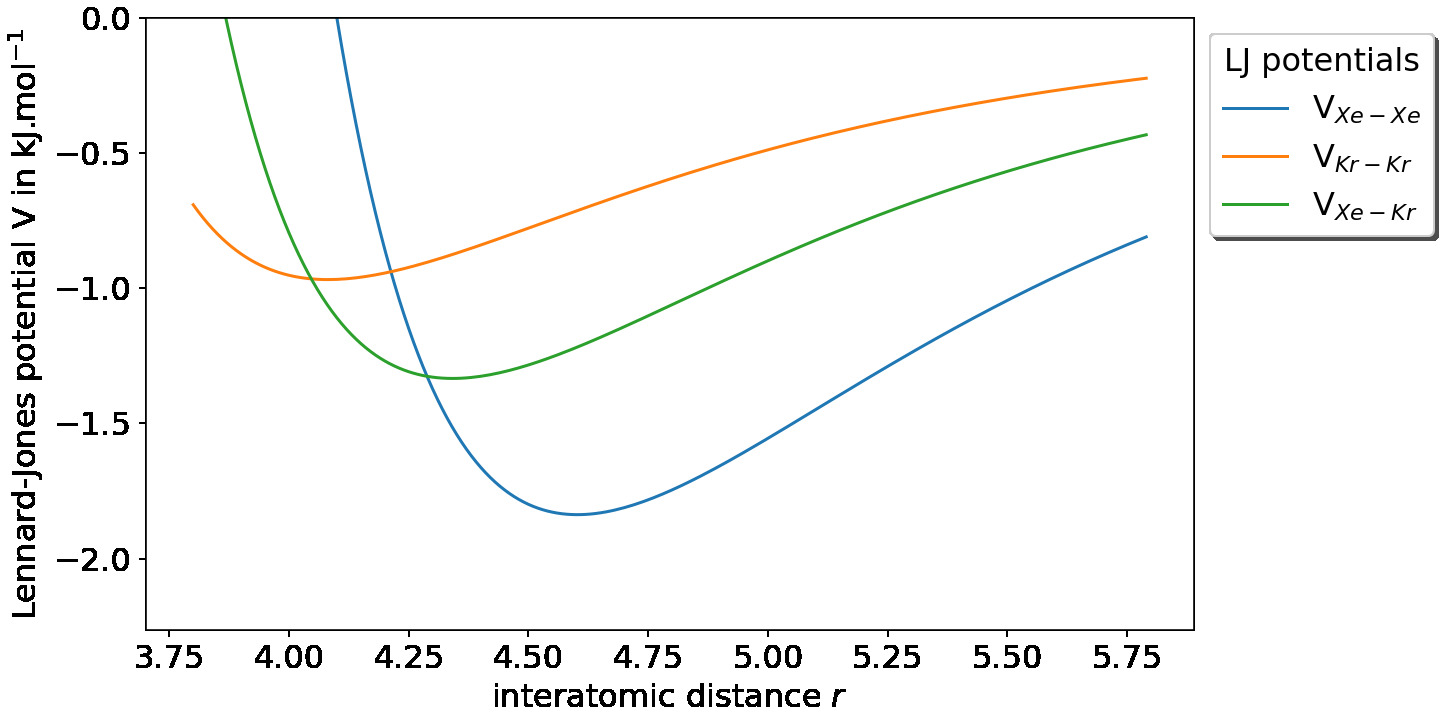
\includegraphics[width=0.6\textwidth]{figures/2-thermo/lennard_jones.jpg}
    \caption{\ The LJ potentials for xenon and krypton interactions. The xenon-xenon interaction is more stabilizing than the krypton-krypton interaction for interatomic distance higher than \SI{4.2}{\angstrom}.}
    \label{fgr:LJ}
  \end{figure}

In the case of KAXQIL, the channels are one-dimensional tubes (see Figure~\ref{fgr:SI:examples:KAXQIL}) and the distance between two adsorption sites is approximately the unit cell parameter along the direction of the tube (\SI{5.6}{\angstrom}). There the selectivity increases with pore filling, for enthalpic reasons, which we can explain by relatively simple reasoning. The Lennard-Jones potentials $V\e{LJ}$ can be estimated for all species at \SI{5.6}{\angstrom}: $V\e{Xe-Xe}=-1.0$\,\si{\kilo\joule\per\mol}, $V\e{Kr-Kr}=-0.3$\,\si{\kilo\joule\per\mol} and $V\e{Xe-Kr}=-0.5$\,\si{\kilo\joule\per\mol}. In a simplistic model where all adsorbed molecules are \SI{5.6}{\angstrom} apart, the cooperative effect is higher between two xenon molecules, which explains the increased selectivity at high uptake. If we look further at the adsorption enthalpy of both xenon and krypton (\emph{c.f.} Table~\ref{tbl:thermo}), they both increase: the guest molecules move from the ``ideal'' adsorption sites, and the guest--guest interactions do not fully compensate. The selectivity change in this material is therefore a consequence of the guest--guest interactions that rearranges the position of the adsorbates inside the nanopores.

\begin{figure*}[h]
  \centering
    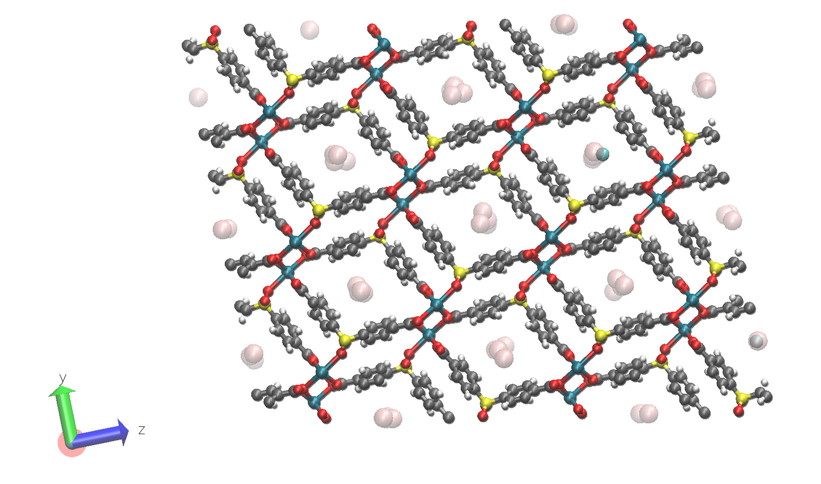
\includegraphics[width=0.45\textwidth]{figures/2-thermo/KAXQIL_clean.jpg}
    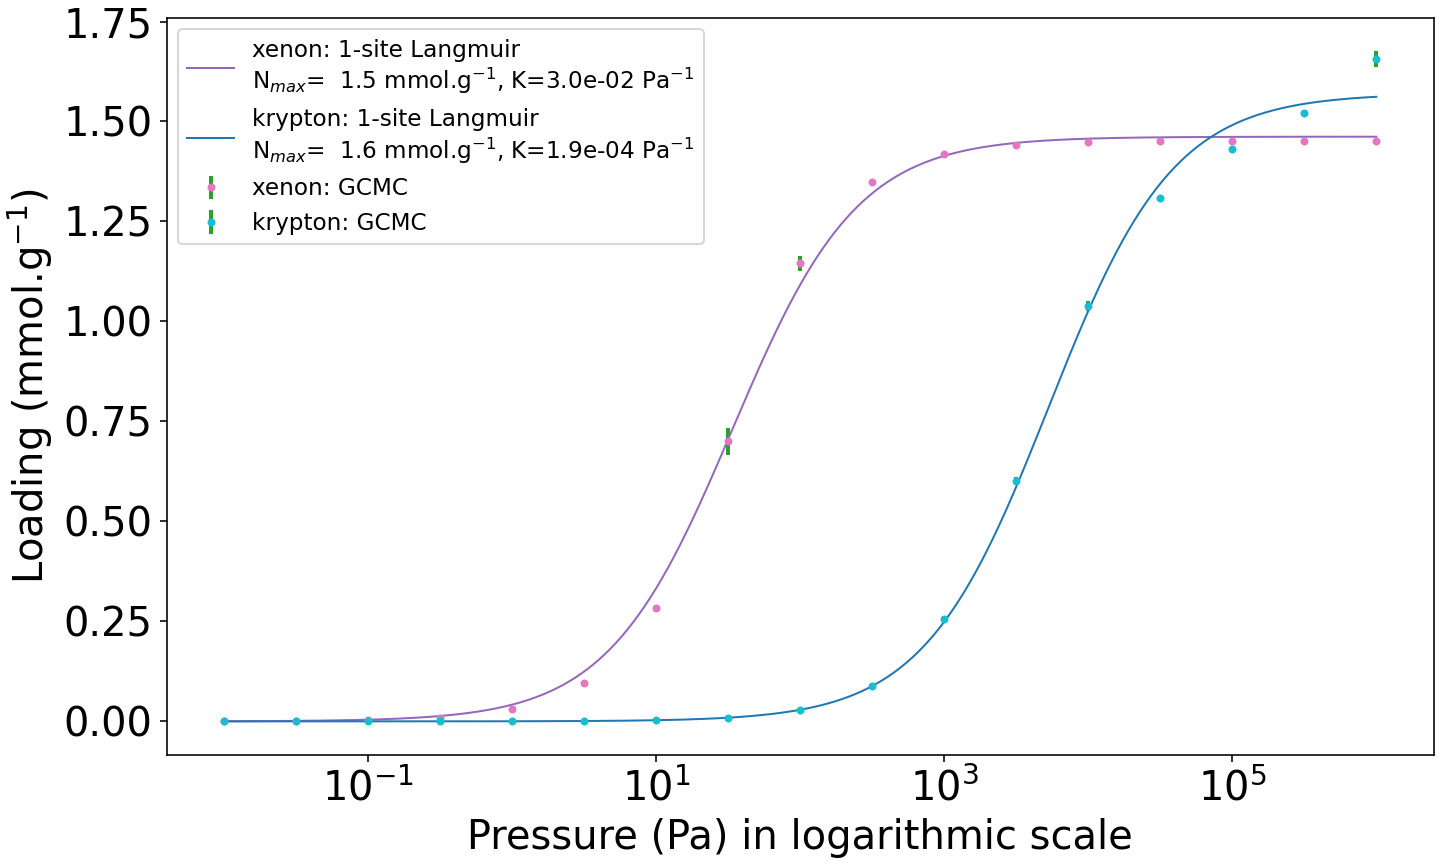
\includegraphics[width=0.45\textwidth]{figures/2-thermo/KAXQIL_clean_isotherm_xenon_krypton_298K.jpg}
    \caption{\ KAXQIL: On the left side, an illustration of a clean version (all solvent removed) of the calcium coordination framework [Ca(SDB)]$\cdot$H$_2$O, where SDB = 4,$4'$-sulfonyldibenzoate loaded with xenon and krypton obtained by GCMC calculations. Color code: Ca in dark cyan, C in gray, O in red, H in white, S in yellow ; Xe in transparent pink and Kr in cyan for the adsorbates. The mono-component isotherms fitted with a 1-site Langmuir model (Equation~\ref{eq:langmuir_1}) for both xenon and krypton at \SI{298}{\kelvin} is represented on the right side.}
    \label{fgr:SI:examples:KAXQIL}
  \end{figure*}

To further corroborate the role of the guest--guest interactions, we look at another material with one-dimensional tubelike channels: JUFBIX, a cobalt(II) coordination polymer based on carboxylic acid linkers (see Figure~\ref{fgr:SI:examples:JUFBIX}).\cite{JUFBIX} The periodicity along the direction of the tubes is much higher at $7.2$\,\si{\angstrom}. The pair interaction energies corresponding to the LJ potentials at this distance are $V\e{Xe-Xe}=-0.24$\,\si{\kilo\joule\per\mol}, $V\e{Kr-Kr}=-0.06$\,\si{\kilo\joule\per\mol} and $V\e{Xe-Kr}=-0.13$\,\si{\kilo\joule\per\mol}. By looking at the adsorption enthalpies (Table \ref{tbl:effect}), these values are too small to affect the position of the adsorbed molecules. At high loading, the distance between adsorbed molecules is high, and every adsorption site is independent of the others. The ambient-pressure selectivity $s\e{1}$ is therefore the same as the low-pressure selectivity $s\e{0}$, since every guest--guest interactions are negligible. It confirms the crucial role of cooperative effects between guest molecules when considering a saturated material.

\begin{figure*}[h]
  \centering
    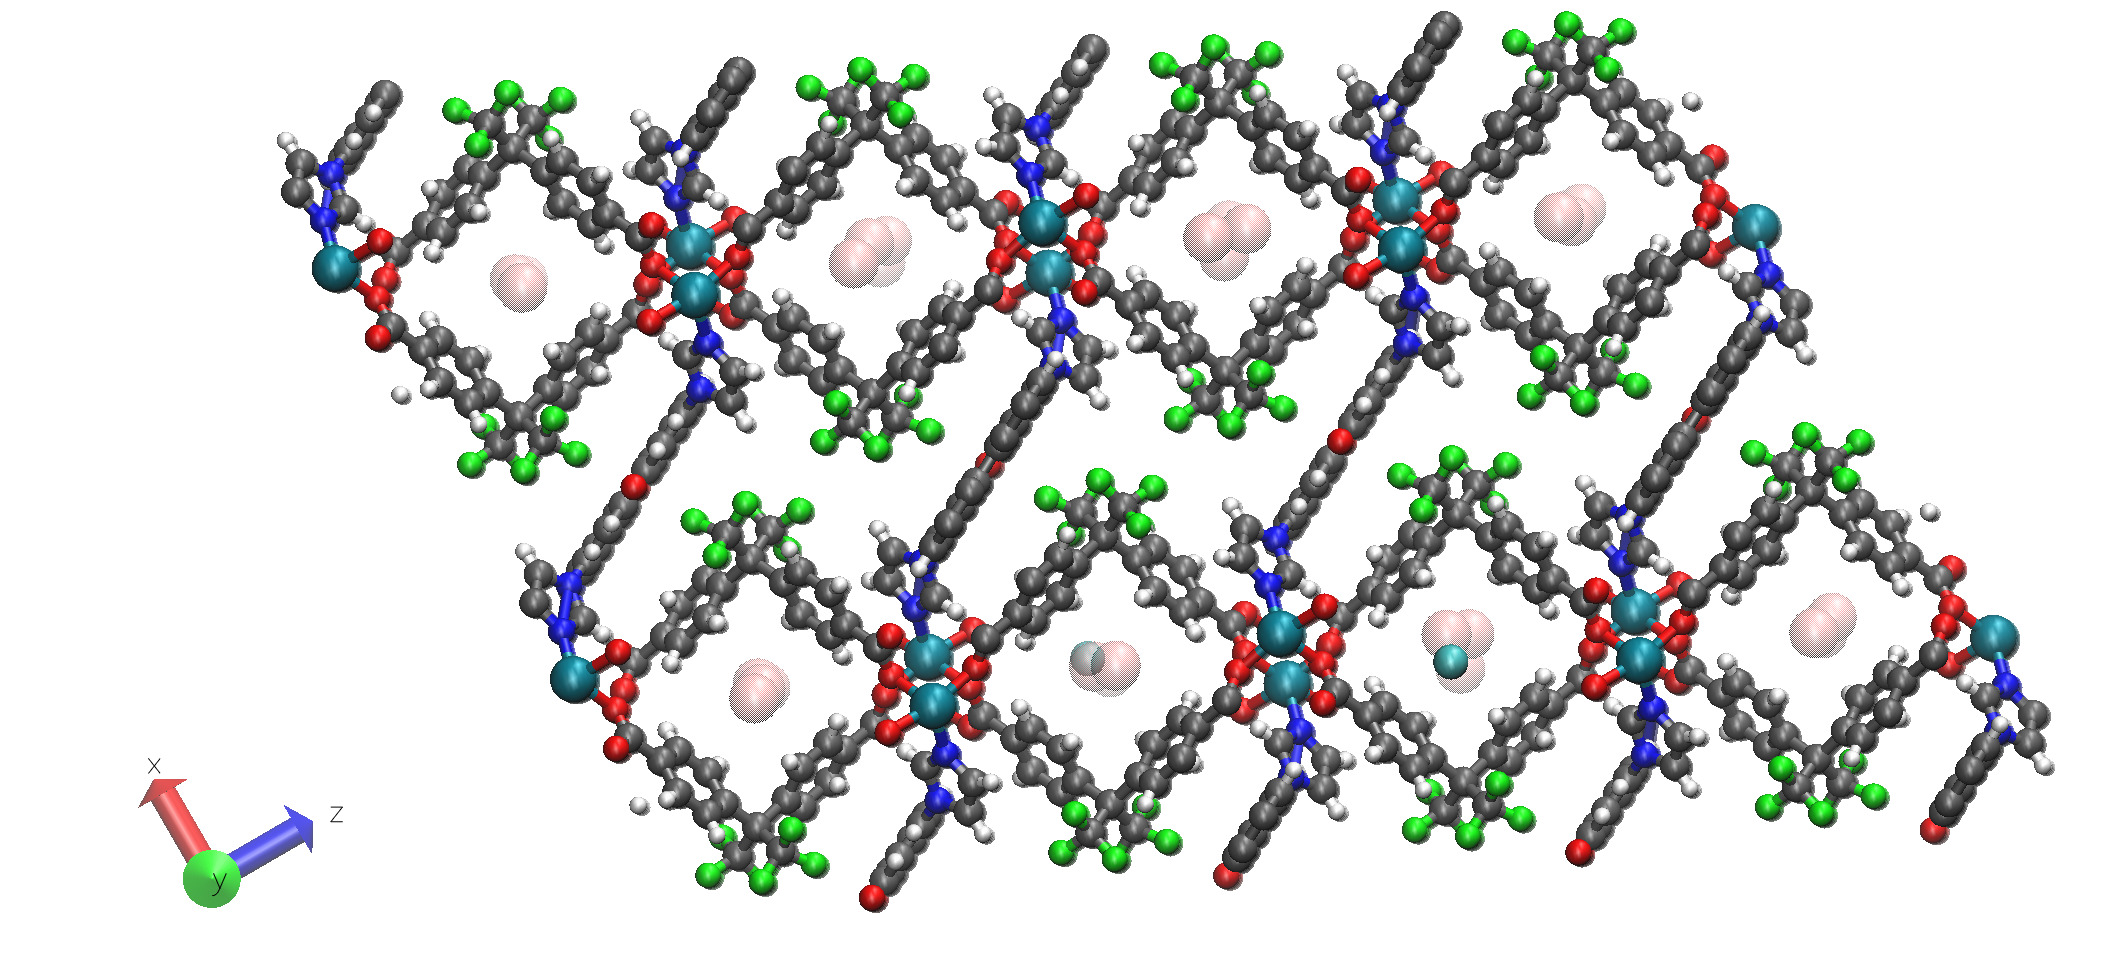
\includegraphics[width=0.45\textwidth]{figures/2-thermo/JUFBIX_clean.jpg}
    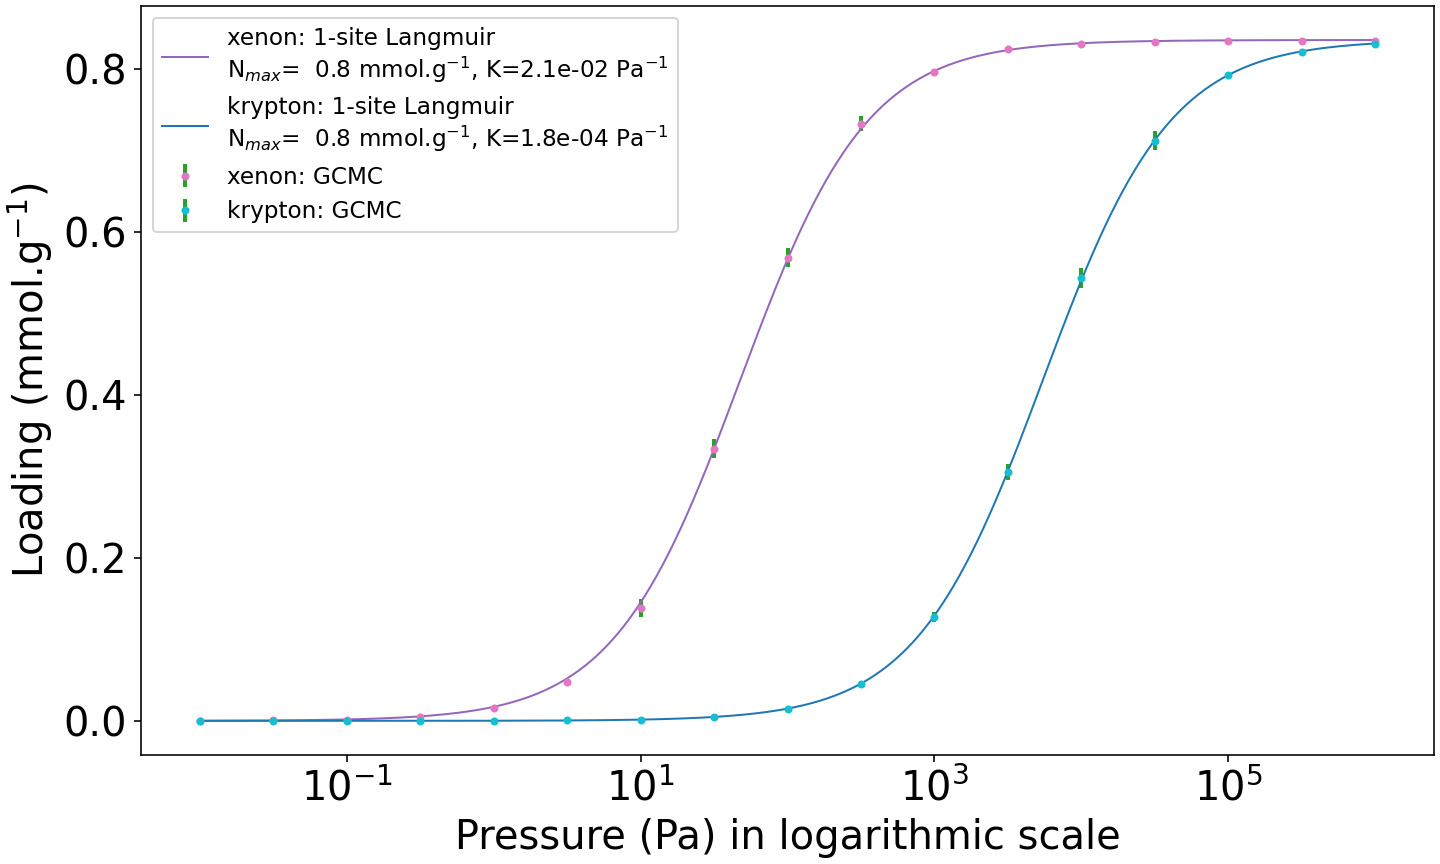
\includegraphics[width=0.45\textwidth]{figures/2-thermo/JUFBIX_clean_isotherm_xenon_krypton_298K.jpg}
    \caption{\ JUFBIX: Representation of a clean version (all solvent removed) of the cobalt(II) coordination framework [Co$_2$(L)(ppda)$_2$]$_2\cdot$H$_2$O, where the ligand L is 2,8-di(1\emph{H}-imidazol-1-yl)dibenzofuran and the carboxylic acid ligand H$_2$ppda is 4,$4'$-(perfluoropropane-2,2-diyl)dibenzoic acid loaded with xenon and krypton obtained by GCMC calculations. Color code: Co in dark cyan, C in gray, O in red, H in white, N in blue, F in green ; Xe in transparent pink and Kr in cyan for the adsorbates. The mono-component isotherms fitted with a 1-site Langmuir model (Equation~\ref{eq:langmuir_1}) for both xenon and krypton at \SI{298}{\kelvin} is represented on the right side.}
    \label{fgr:SI:examples:JUFBIX}
  \end{figure*}

GOMREG and JAVTAC are frameworks that belong to the second category of materials, with a moderate decrease in selectivity from low to ambient pressure. In GOMREG, the channels are composed of one-dimensional tubes larger than the ones found in KAXQIL or JUFBIX (see Figure~\ref{fgr:SI:examples:GOMREG} and Table~\ref{tbl:effect}). The adsorption sites are alternating from left to right inside the channel, and the adsorbed molecules organize in a ``zigzag'' pattern. Looking at the adsorption enthalpies, we see that both xenon and krypton have lower enthalpies by a similar margin, suggesting an equivalent stabilization for both atoms, hence the enthalpic contribution to the selectivity change is close to 1.
Since krypton is smaller and less strongly tied on its adsorption site than xenon, it has more available space inside the pore space. This gives an entropic advantage to the Kr, seen in the entropic contribution $k\e{S}$ of $0.64$ in Table~\ref{tbl:effect}. This indicates that even if enthalpic considerations mainly explain the observed changes at a statistical level, as discussed in the previous sections, for individual cases entropic considerations can be a strong factor in pressure-dependent selectivity.

\begin{figure*}[h]
  \centering
    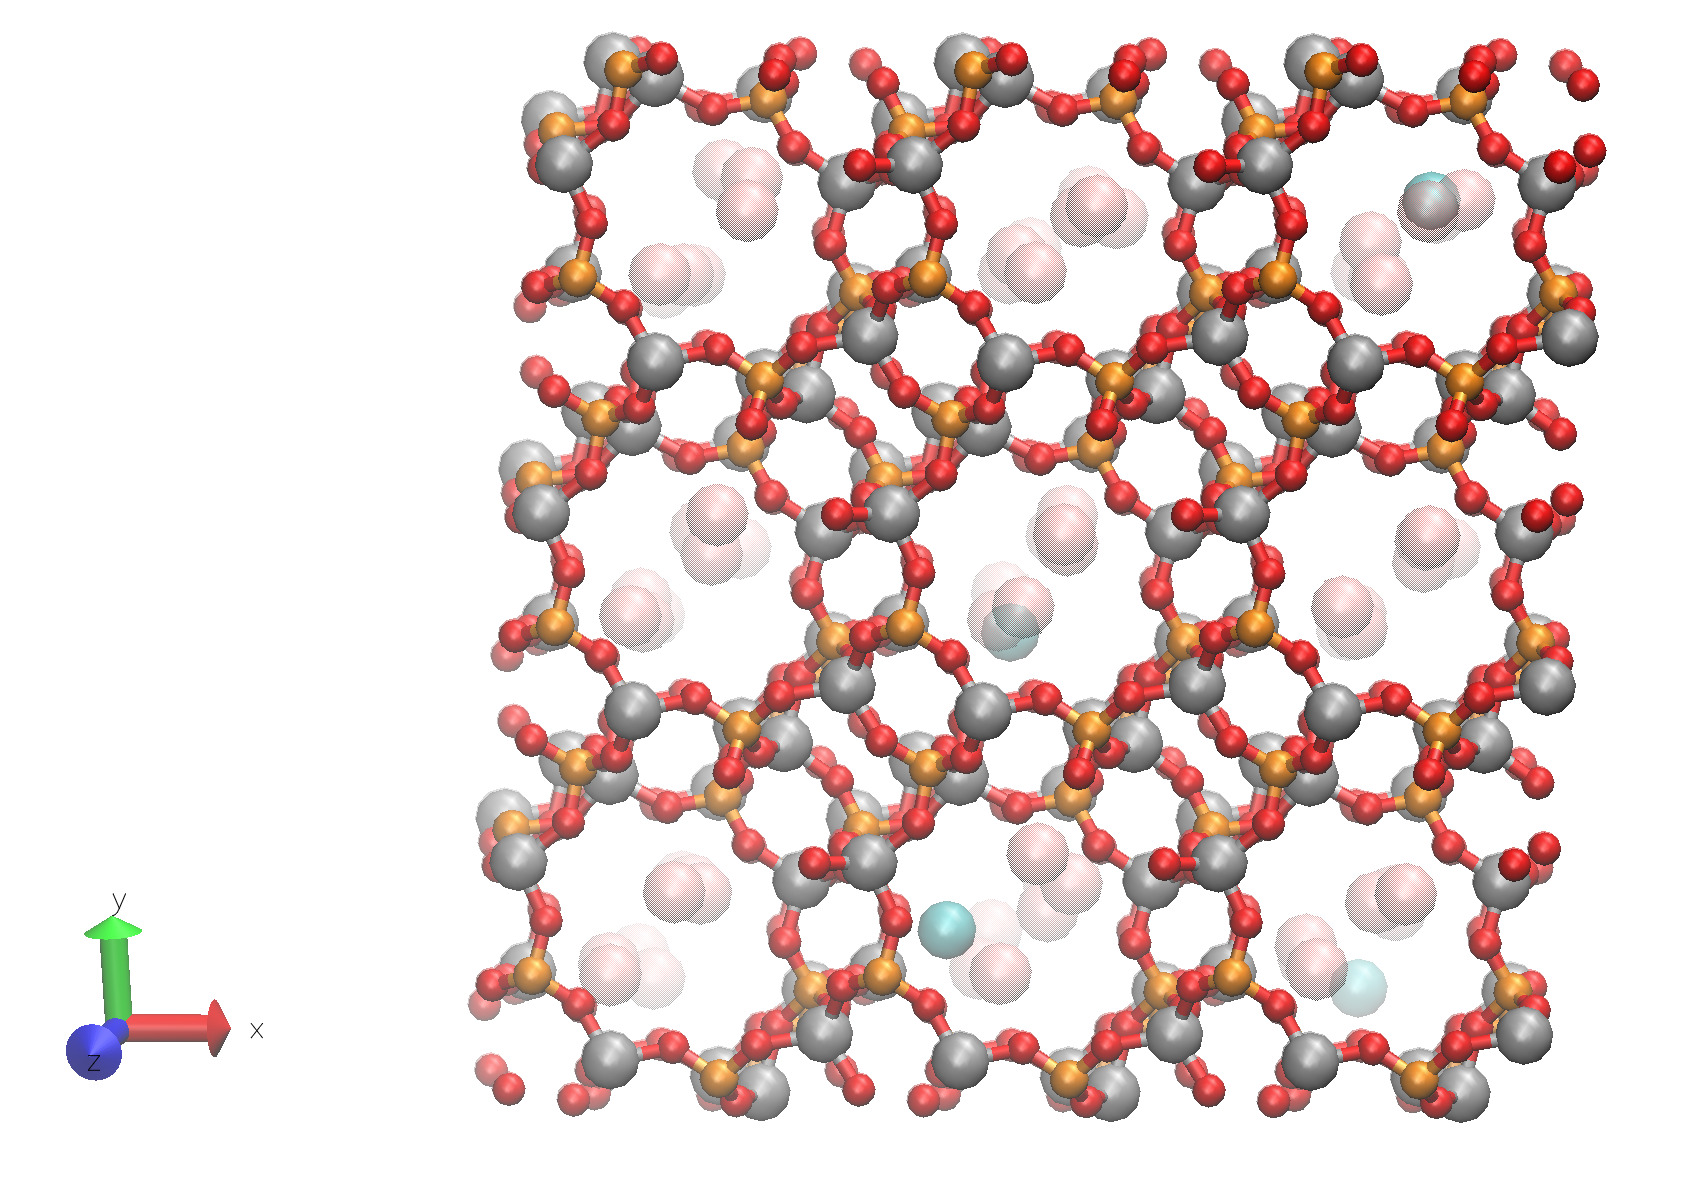
\includegraphics[width=0.45\textwidth]{figures/2-thermo/GOMREG_clean.jpg}
    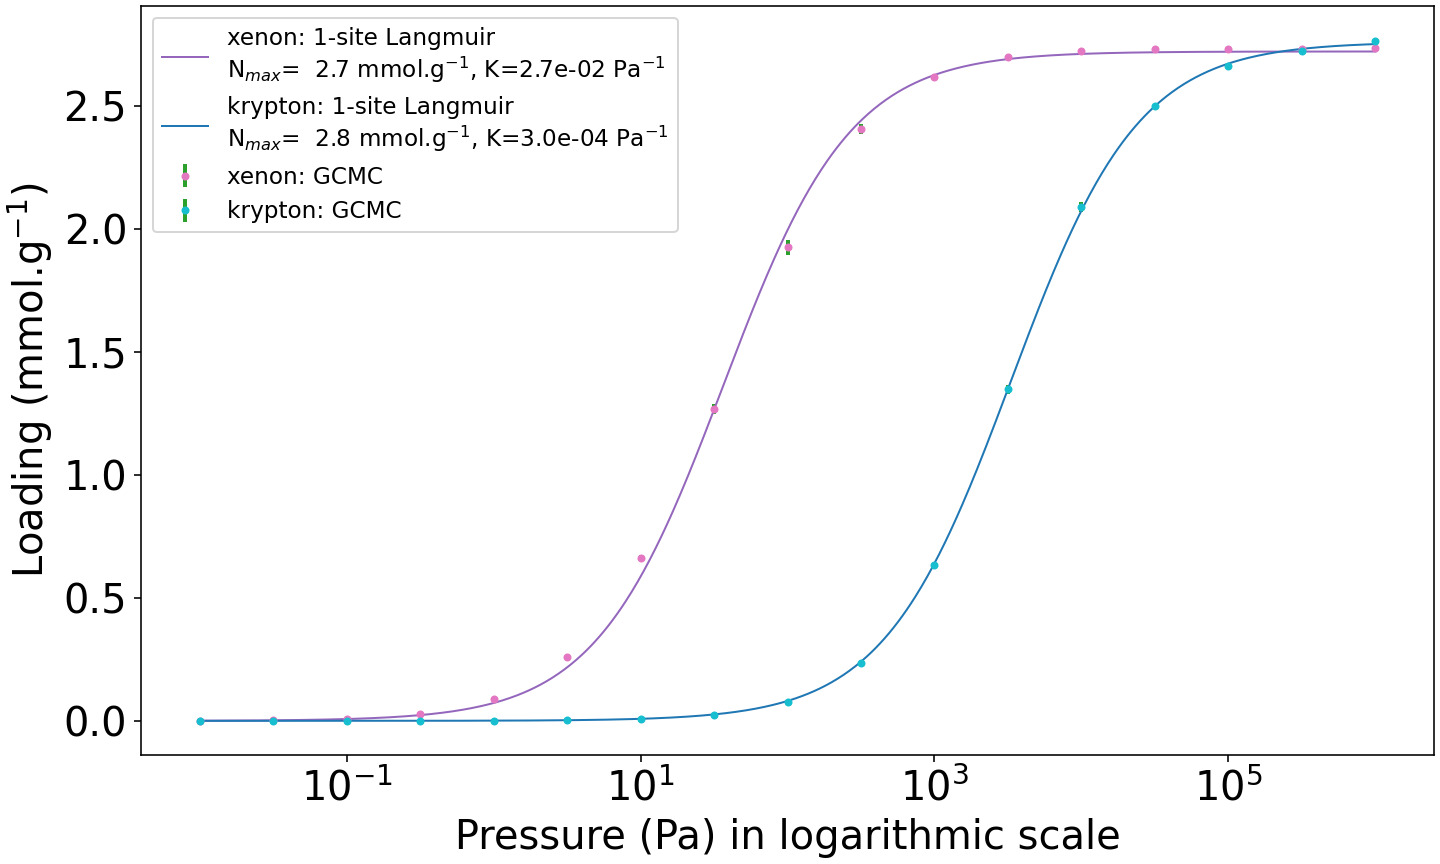
\includegraphics[width=0.45\textwidth]{figures/2-thermo/GOMREG_clean_isotherm_xenon_krypton_298K.jpg}
    \caption{\ GOMREG: Representation of a clean version (all solvent removed) of this aluminophosphate AlPO$_4$-$n$ that has a zeotype LAU topology with one-dimensional 10-ring channels loaded with xenon and krypton obtained by GCMC calculations. Color code: Al in silver, P in orange, O in red ; Xe in transparent pink and Kr in cyan for the adsorbates. The mono-component isotherms fitted with a 1-site Langmuir model (Equation~\ref{eq:langmuir_1}) for both xenon and krypton at \SI{298}{\kelvin} is represented on the right side.}
    \label{fgr:SI:examples:GOMREG}
  \end{figure*}

The remaining materials discussed here form a third category, with a strong decrease in selectivity from low to ambient pressure. We look at several phenomena that can be at the root of this decrease, which is important for screening studies as it can limit the working performance of a material that appears to be a ``top performer'' based on zero-pressure screening.


For example, GOMRAC has a similar structure compared to GOMREG (see Figure~\ref{fgr:SI:examples:GOMRAC}), except for the fact that the pores and channels are smaller (see the values of the GCD, and the PLD, in Table~\ref{tbl:effect}). The distances between the adsorbed molecules --- in their ideal sites --- are then consequently smaller. At such distances, we can assume that the interactions between adsorbates become more stabilizing for krypton than for xenon molecules in GOMRAC (see LJ potentials at distance lower than \SI{4.2}{\angstrom} in the Figure~\ref{fgr:LJ}), which translates into an enthalpic contribution $k\e{H}$ of $0.58$. Moreover, this is compatible with the equivalent guest--guest interactions in GOMREG, as previously discussed. It explains why the difference between the adsorption enthalpies becomes smaller for GOMRAC, whereas it stays the same for GOMREG (between low and ambient pressure). This further validates the crucial role of the interactions between adsorbed molecules, and their relationship with the guest-guest distances when considering a high loading condition.

\begin{figure*}[h]
  \centering
    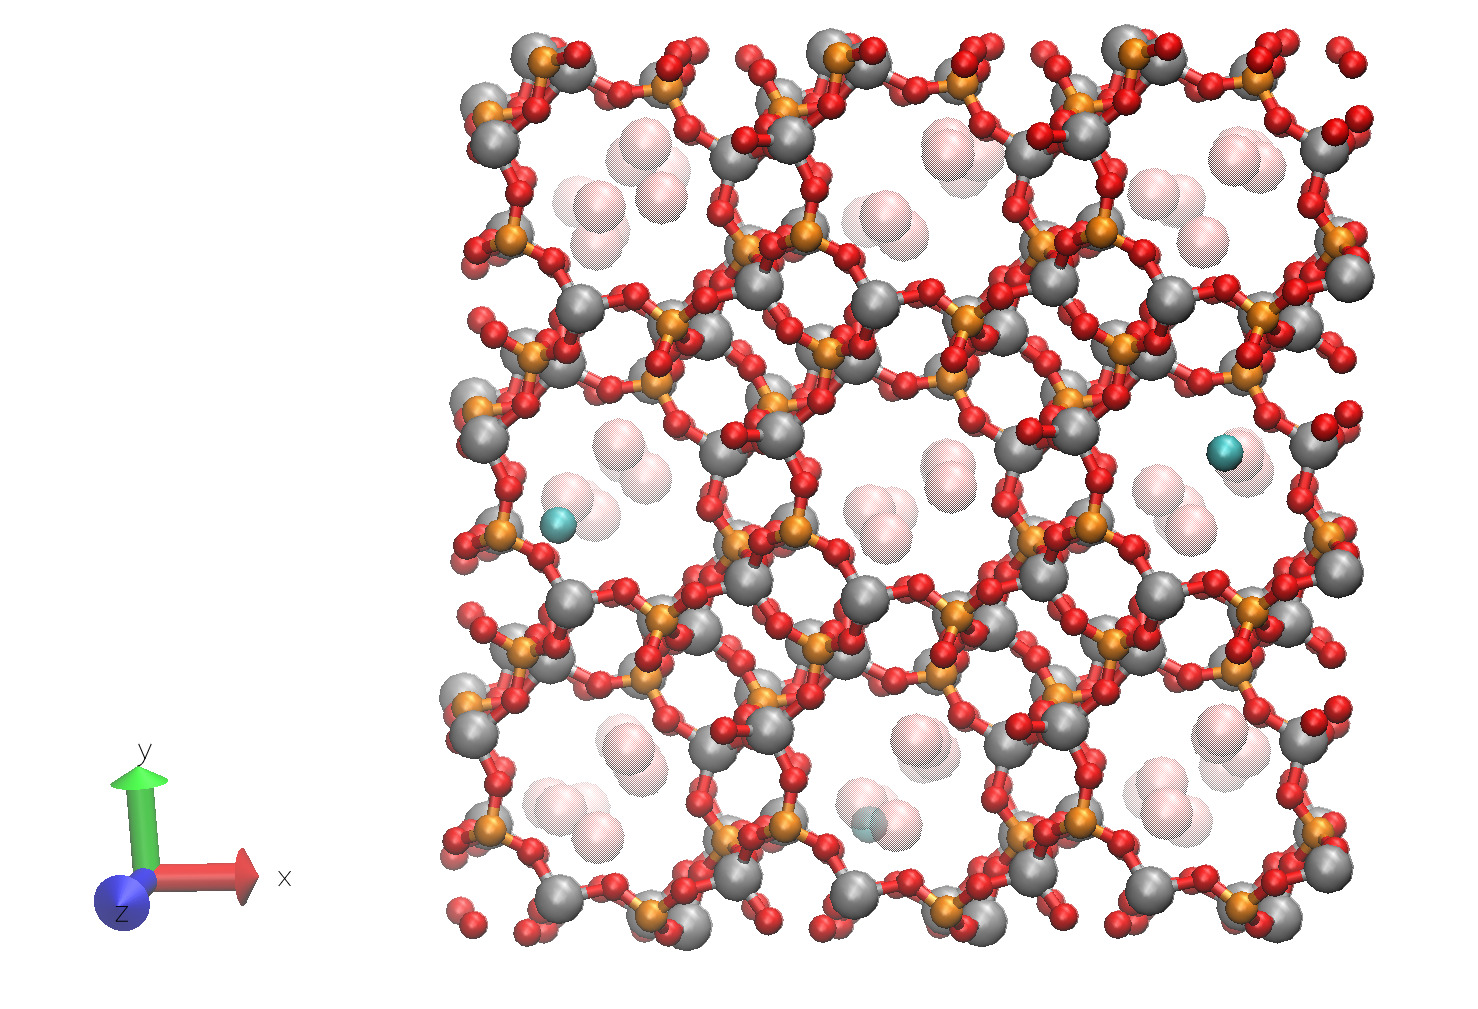
\includegraphics[width=0.45\textwidth]{figures/2-thermo/GOMRAC_clean.jpg}
    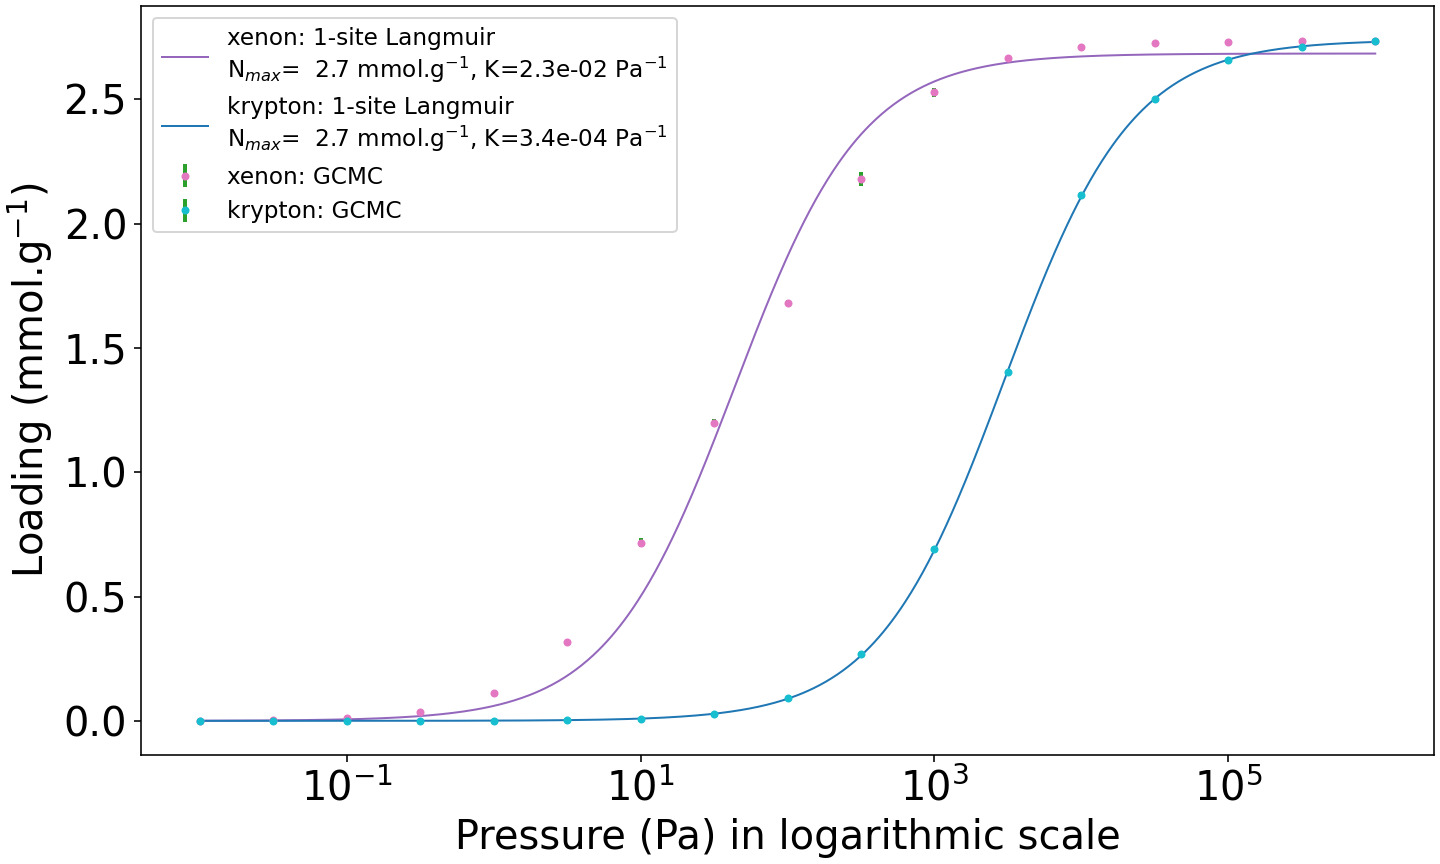
\includegraphics[width=0.45\textwidth]{figures/2-thermo/GOMRAC_clean_isotherm_xenon_krypton_298K.jpg}
    \caption{\ GOMRAC: Representation of a clean version (all solvent removed) of this aluminophosphate AlPO$_4$-$n$ that has a zeotype LAU topology with one-dimensional 10-ring channels loaded with xenon and krypton obtained by GCMC calculations. Color code: Al in silver, P in orange, O in red ; Xe in transparent pink and Kr in cyan for the adsorbates. The mono-component isotherms fitted with a 1-site Langmuir model (Equation~\ref{eq:langmuir_1}) for both xenon and krypton at \SI{298}{\kelvin} is represented on the right side. It seems that this aluminophosphate is just a smaller version of GOMREG.}
    \label{fgr:SI:examples:GOMRAC}
  \end{figure*}

If we look at the case of MISQIQ, we see that the pure-component Xe isotherm in Figure~\ref{fgr:MISQIQ} cannot be fitted by a single-site Langmuir isotherm, but is well fitted by a two-site Langmuir model (see Figure~\ref{fgr:MISQIQ}). Visual inspection of the adsorbed density at various loadings shows that this is not a second, separate adsorption site that is populated at high loading: instead, the second step in the isotherm (representing about {20\%} of the uptake at full loading) is associated with a reorganization of the adsorbate molecules occurs at high loading, accompanying a contraction of the interatomic distances. In this case, the potential for a reorganization of the adsorbate in the material's nanopores leads to the change in selectivity. This reorganization can be detected on the basis of the xenon isotherm alone, and has a major role in the selectivity at ambient pressure. This repacking of the adsorbed phase is linked to a strong entropic effect, and also impacts the enthalpic contribution to selectivity.

\begin{figure*}[t]
  \centering
    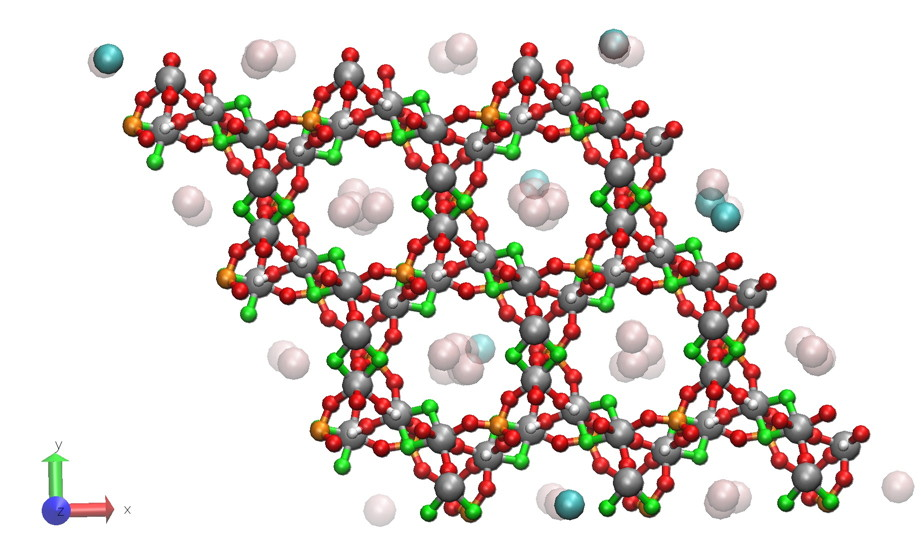
\includegraphics[width=0.48\textwidth]{figures/2-thermo/MISQIQ_clean.jpg}\hfill
    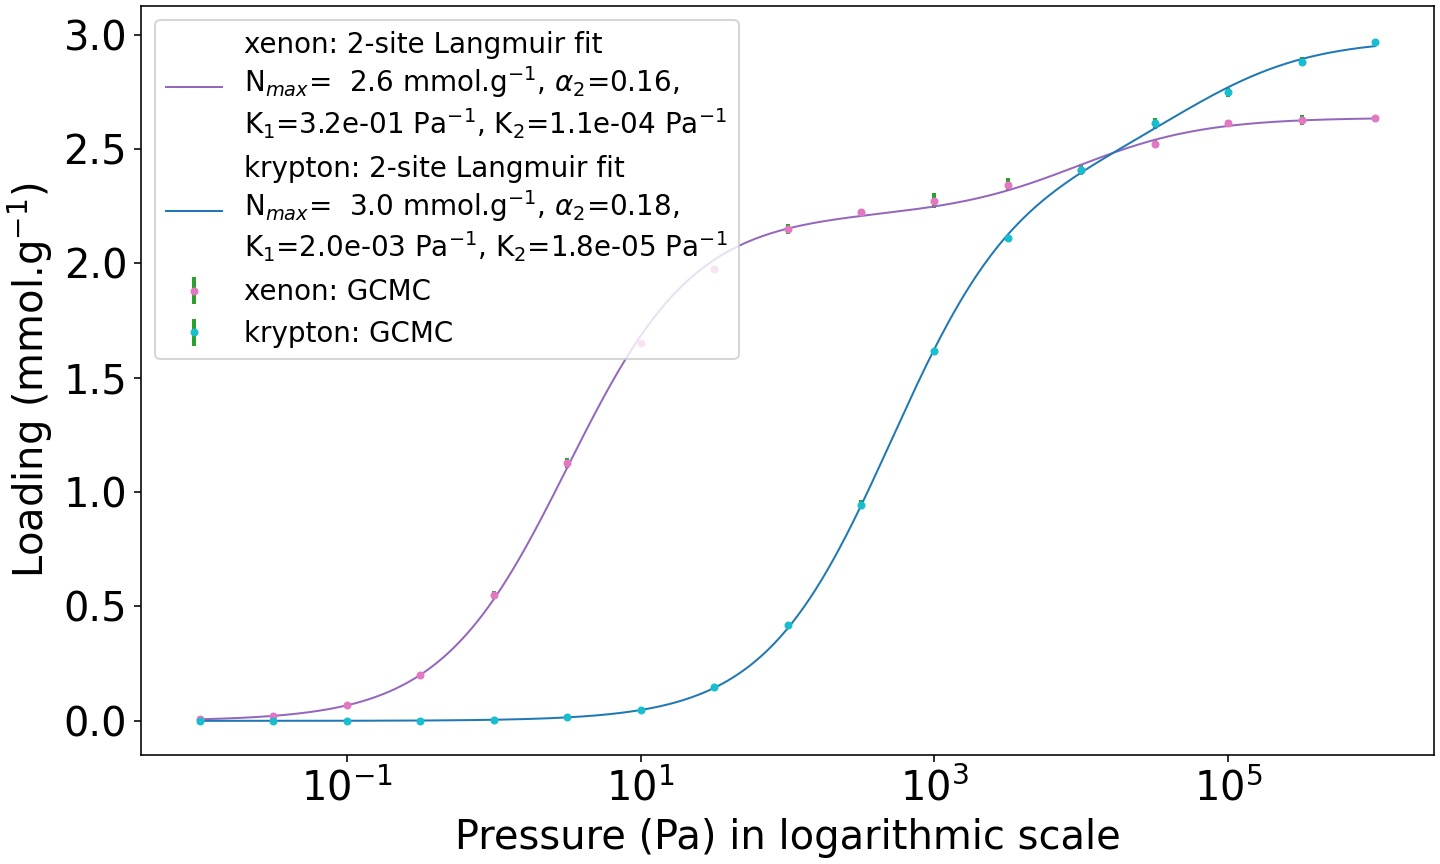
\includegraphics[width=0.48\textwidth]{figures/2-thermo/MISQIQ_clean_isotherm_xenon_krypton_298K.jpg}
    \caption{Representation of a chiral open-framework fluoroaluminophosphate [C$_4$N$_3$H$_{16}$]$\cdot$[Al$_6$P$_3$O$_{12}$F$_6$(OH)$_6$] denoted AlPO-JU89 (referenced MISQIQ in the Cambridge structural database), which has been loaded with xenon and krypton in a GCMC simulation, on the left side.\cite{MISQIQ} Color code: Al in silver, P in orange, O in red, H in white and F in green for the framework; and Xe in transparent pink and Kr in cyan for the adsorbates. The pure-component isotherms fitted with a 2-site Langmuir model (Equation~\ref{eq:langmuir_2}) for both xenon and krypton at \SI{298}{\kelvin} on the right side.}
    \label{fgr:MISQIQ}
  \end{figure*}

More extreme cases of selectivity drop can occur when more than one site is available, as is the case for materials BAEDTA01, VIWMOF, LUDLAZ, WOJJOV, and VAPBIZ. The pure-component isotherms and the representation of the materials loaded in xenon and krypton molecules (presented in the supporting information of the Ref.~\ref{Ren_2021} Figures~S19-23) confirm the existence of at least two distinct adsorption sites in each material. The most selective sites (i.e., the most favorable for Xe) are filled in priority at low loading, and the less selective sites will then be populated when the pressure increases, leading to a net selectivity drop at ambient pressure for these materials. The different types of adsorption sites, and therefore the potential for a drop in Xe/Kr selectivity (at non-zero pressure) is a factor that could be explicitly included in screening of pure-component isotherms, without the need for explicit multi-component GCMC simulations.

\subsection{Conclusion and introduction to the follow-up studies}

In the current state of the art on Xe/Kr separation by adsorption in nanoporous materials, many studies have focused on the determination of structure/property relationships, the description of theoretical limits of performance, and the identification of top-performing materials, whether for existing experimental structures or for novel hypothetical structures yet to be synthesized. Here, we provide a study based on a high-throughput screening of the adsorption of Xe, Kr, and Xe/Kr mixtures in 12,020 experimental open-framework materials, in order to provide a better comprehension of the thermodynamics behind Xe/Kr separation in nanoporous materials and the microscopic origins of Xe/Kr selectivity at both low and ambient pressure. 

The statistical correlation found between Henry's constant for Xe and Xe/Kr selectivity showed that the most selective materials are those with the highest affinity for xenon. To some degree of accuracy, we conclude that directly screening for Kr adsorption or for  xenon adsorption free energy may not be necessary for a coarse-grained evaluation of a nanoporous framework selectivity. This could help build more efficient screening methodologies, for example with multistage studies with a first rough selection on Henry's constant at a low computational cost, followed by more expensive GCMC simulations on the selected materials (a gain that can be between 5 and 10-fold in our setup). Furthermore, inspection of the correlations between enthalpy and entropy contributions at low pressure showed that the adsorption-based separation process in the open frameworks studied is mainly enthalpic in nature. We intend to extend the study in the future to other classes of nanoporous materials beyond MOFs, including covalent organic frameworks, porous aromatic frameworks, purely inorganic porous frameworks such as zeolites, but also amorphous porous materials such as porous polymer membranes.

In order to use nanoporous materials to separate xenon from krypton, pressure swing adsorption (PSA) processes have been widely offered: pressure is therefore a crucial thermodynamic variable in the separation cycle. Here, we studied the difference of selectivity between a system under very low pressure (at the zero loading limit, which is calculated at relatively low computational cost) and a system at ambient pressure (closer to working conditions, but obtained at higher simulation cost). We demonstrated that the selectivity could be highly dependent on the pressure, with high low-pressure selectivity that could be maintained in some materials at ambient-pressure selectivity, while in others there would be a large drop in selectivity: a high ambient-pressure selectivity requires high low-pressure selectivity, but the reverse does not hold.

Using a thermodynamic approach to describe the separation selectivity, we showed that the differences in selectivity between the different pressures (and therefore different loading regimes of the frameworks) are mainly explained by the evolution of the adsorption enthalpies for Xe and Kr. By focusing on specific examples, we uncovered the microscopic origins of these selectivity changes, and related them to the relative roles of host--guest and guest--guest interactions. Population of different adsorption sites, or repacking of the adsorbed phase at higher loading, can lead to drastic changes in the overall selectivity. The mechanisms behind selectivity at high pressure are complex and unique to each framework, requiring a good understanding of the interactions between guest molecules constrained in the nanopores. Nevertheless, our classification of the interactions at play can help in the future to design more efficient high-throughput screening procedures.

For instance, the essentially enthalpic nature of the xenon/krypton separation process supports the need for more efficient ways of sampling the interaction energies and using them as cheap descriptors to tackle more and more numerous structures. In the next chapter, we will go over different ways of evaluating the adsorption enthalpy by comparing the computation time required and the accuracies of each of them. Finally, the influence of the partial pressure through the change in composition or in pressure questions the possible use of infinite dilution thermodynamic quantities to predict the selectivity at any pressure (GCMC). Many studies have focused on predicting the results of GCMC simulations;\cite{Simon_2015,Shi_2023,Kang_2023,Li_2023} by using this new angle, can we achieve good results in predicting GCMC values?

\textbf{Data Availability:} \url{https://github.com/fxcoudert/citable-data/tree/master/132-Ren_FaradayDiscuss_2021}

\OnlyInSubfile{\printglobalbibliography}

\end{document}
